%%%%%%%%%%%%%%%%%%%%%%%%%%%%%%%%%%%%%%%%%
% JM Thesis
% can be compiled with PDFLaTex
% options in structure.tex
%%%%%%%%%%%%%%%%%%%%%%%%%%%%%%%%%%%%%%%%%

%----------------------------------------------------------------------------------------
%	PACKAGES AND OTHER DOCUMENT CONFIGURATIONS
%----------------------------------------------------------------------------------------

%\documentclass[12pt,letterpaper,twoside,fleqn]{memoir}
\documentclass[12pt,a4paper,twoside,fleqn]{memoir}
% Change font size here (allowable values are 9pt-12pt), change the paper size, specify one or two sided printing and specify whether to show trimming lines

%\documentclass[10pt,a4paper,twoside]{memoir} % Change font size here (allowable values are 9pt-12pt), change the paper size, specify one or two sided printing and specify whether to show trimming lines

\input{structure_notrim_small_margins.tex} % Include the file containing the code defining the structure and style of the document
%\input{structure_book_08reduction.tex} % Include the file containing the code defining the structure and style of the document

%------------------------------------------------
% Thesis Information

\title{Life History, Behaviour and Responses to Environmental Changes} % Thesis title

\author{Joan Maspons Ventura % Author name
  \href{https://orcid.org/0000-0003-2286-8727}{\includegraphics[width=8pt,keepaspectratio=true]{./Figures/intro/orcid_logo.png}}
}

\date{Juny de 2021} % The date

\newcommand{\institution}{Universitat Autònoma de Barcelona\xspace} % University/institution name

\newcommand{\department}{Centre de Recerca Ecològica i Aplicacions Forestals\xspace} % Department name

%------------------------------------------------
% Fonts

\renewcommand*{\acffont}[1]{{\normalsize\itshape #1}} % Font style for the acronym text (e.g. Do It Yourself)
\renewcommand*{\acfsfont}[1]{{\normalsize\upshape #1}} % Font style for the acronym in bracket (e.g. (DIY))

%------------------------------------------------
% Hyphenations

\hyphenation{} % Specify custom hyphenation points in words with dashes where you would like hyphenation to occur, or alternatively, don't put any dashes in a word to stop hyphenation altogether

%----------------------------------------------------------------------------------------
%	TITLE PAGE
%----------------------------------------------------------------------------------------

\renewcommand{\maketitlehooka}{
\centering
% institution logo(s)
\includegraphics[width=.75\textwidth]{./Figures/intro/CREAF-UAB.png}\\[.8cm]
\institution\\ % Print institution name
\emph{\department}\\[.2cm] % Print department name
DOCTORAT EN ECOLOGIA TERRESTRE % Degree or other information
\par
\hrulefill
\vfill}
\renewcommand{\maketitlehookb}{\vfill}
\renewcommand{\maketitlehookc}{
\vfill
\begin{flushleft}
Directors:\\
\textbf{Dr. Daniel Sol Rueda}\\ % Director's name
\textbf{Dr. Roberto Molowny Horas}\\[.3cm] % Director's name
Comissió de seguiment:\\
\textbf{Dr. Maria Mayol Martínez}\\ % Advisor's/supervisor's name
\textbf{Dr. Frederic Bartomeus Ferré}\\ % Advisor's/supervisor's name
\textbf{Dr. Javier Retana Alumbreros}\\[.3cm] % Advisor's/supervisor's name
Supervisora del programa de doctorat:\\
\textbf{Dr. Anna Ávila Castell} % Doctoral program supervisor's name
\end{flushleft}
\vfill}
\preauthor{\begin{flushright}Memòria presentada per:\\\bfseries} % Text prior to the author name - right aligned and bold
\postauthor{\end{flushright}} % After the author name, stop right alignment

%----------------------------------------------------------------------------------------

\makeindex % Write an index file

\begin{document}

\begin{titlingpage}
\maketitle % Print the title page
\end{titlingpage}

\frontmatter % Use roman page numbering style (i, ii, iii, iv...) for the pre-content pages

%----------------------------------------------------------------------------------------
%	PREFACE
%----------------------------------------------------------------------------------------

\selectlanguage{catalan}

\vspace*{.4\textheight}

\begin{flushright}
Per la Teresa
\end{flushright}


\cleardoublepage

\section*{Agraiments}

% TODO: Agraiments

\hfill

\begin{flushright}
%\textsc{\theauthor}\\
Can Maspons de la Vall\\
Juny de 2021
\end{flushright}

\vspace*{\fill}
\hrulefill

Aquesta tesi ha estat finançada mitjançant una beca predoctoral per a la
formació de personal investigador (FPI) BES-2011-043668, concedida pel
Ministerio de Educación y Ciencia a través del projecte de recerca
CGL2010-21838.

\cleardoublepage % Force a break to an even page


%----------------------------------------------------------------------------------------
%	ABSTRACT
%----------------------------------------------------------------------------------------

\selectlanguage{catalan}
% \renewcommand{\catalanabstractname}{Resum} % to avoid installing texlive-lang-spanish for babel-catalan

\begin{abstract}
A la natura trobem una extraordinària diversitat d'estratègies vitals, les
diferents maneres en què les espècies optimitzen els seus recursos limitats en
els diferents components de l'eficàcia biològica, com ara la reproducció, el
desenvolupament o la supervivència.
En un mon canviant com el nostre, oimés en un context de canvis ambientals
ràpids induïts pels humans, és de vital importància entendre com les espècies
poden adaptar-se a les noves condicions tenint en compte les restriccions de
l'evolució dels trets deguts a la història filogenètica i als balanços entre els
diferents trets.
El marc teòric de les estratègies vitals permet veure de forma integrada
l'evolució dels trets de les espècies en funció de les pressions de selecció de
l'ambient.
En el cas dels animals, una forma que tenen de fer front als canvis és
mitjançant la plasticitat del comportament, que recentment s'ha vist que està
lligada a les estratègies vitals en el què anomenem síndromes del ritme de vida.

L'objectiu d'aquesta tesi és contribuir a entendre com les espècies responen
als canvis i quin paper hi juguen les estratègies vitals i el comportament.
En el primer capítol, descric els principals eixos de variació de les
estratègies vitals en ocells posant èmfasi en els efectes demogràfics de l'eix
ràpid-lent (\textit{fast-slow} en anglès) i descrivint altres eixos menys
estudiats com ara la iteroparitat o la mida relativa dels ous (Capítol
\ref{ch:LHaxes}).
A continuació, exploro els efectes i les interaccions entre les estratègies
vitals i el comportament en un context de canvi ambiental mitjançant un model
estocàstic basat en individus que mostra que els beneficis de l'aprenentatge
són contingents a l'estratègia vital (Capítol \ref{ch:LH-Behaviour model}).
Finalment, descric l'existència d'interaccions entre estratègies vitals i el
comportament mitjançant mètodes comparatius amb dades d'ocells que mostren que
les espècies de vida lenta tendeixen a prendre menys riscos i, alhora,
aquest comportament és flexible i s'ajusta quan es troben en nous ambients com
ara les àreas urbanes (Capítol \ref{ch:POLS}).

\end{abstract}

\clearpage

\selectlanguage{english}

\begin{abstract}
In nature we find an extraordinary diversity of life history strategies, the
different ways in which species optimize their limited resources in different
components of the fitness, such as reproduction, development or survival.
In a changing world like ours, even more in a context of human-induced
rapid environmental change, it is vital to understand how species can adapt to
the new conditions taking into account the constraints of
the evolution of traits due to phylogenetic history and trade-offs between
different traits.
The framework of the life history theory allows us to view the evolution of
species traits in an integrated way as a function of the selection pressures
from the environment.
In the case of animals, one way they have to deal with changes is
through the plasticity of behavior, which has recently been seen to be linked
to the life histories in what we call peace of life syndromes.

The aim of this thesis is to contribute to the understanding of how species
respond to changes and what is the role of the life histories and behavior.
In the first chapter, I describe the main axes of variation of the life history
in birds emphasising the demographic effects of the fast-slow axis and
describing other less studied axes such as the iteroparity or the relative egg
size (Chapter\ref{ch:LHaxes}).
Then, I explore the effects and the interactions between life history and
behaviour in a context of environmental change using a stochastic individual
based model showing that the benefits of learning are contingent on life
history (Chapter \ref{ch:LH-Behaviour model}).
Finally, I describe the existence of interactions between life history and
behaviour by means of comparative methods using bird's data showing that
slow-lived species tend to be more risk-averse and, at the same time,
this behaviour is plastic and is adjusted in new environments like urban areas
(Chapter \ref{ch:POLS}).
\end{abstract}

\clearpage
% \cleartoverso % Force a break to an even page

%----------------------------------------------------------------------------------------
%	chapter status
%----------------------------------------------------------------------------------------

\section*{Article references}

\begin{itemize}
  \item \textbf{Chapter 2:} \\
  Maspons, J. \& D. Sol. 2021. Revisiting the fast-slow continuum of life history variation in birds. Manuscript in preparation.
  
  \item \textbf{Chapter 3:} \\
  Maspons, J., R. Molowny‐Horas, \& D. Sol. 2019. Behaviour, life history and persistence in novel environments. \textit{Phyl. Trans. R. Soc. B} 374:20180056. \href{http://dx.doi.org/10.1098/rstb.2018.0056}{doi:10.1098/rstb.2018.0056}
  
  \item \textbf{Chapter 4:} \\
  Sol, D., J. Maspons, A. Gonzalez-Voyer, I. Morales-Castilla, L. Z. Garamszegi, A. P. M\o{}ller. 2016 Risk-taking behavior, urbanization and the pace of life in birds. \textit{Behav. Ecol. Sociobiol}. 72, 59. \href{http://dx.doi.org/10.1007/s00265-018-2463-0}{doi:10.1007/s00265-018-2463-0}

  %TODO: \item \textbf{Chapter 5:} \\ Life history and environment
\end{itemize}

\bigskip

\begin{center}
 \includegraphics{./Figures/intro/CC_BY-NC-SA.png}
\end{center}

\textbf{CAT:} Life History, Behaviour and Responses to Environmental Changes © 2021 per Joan
Maspons Ventura està subjecta a una llicència
Reconeixement-NoComercial-CompartirIgual 4.0 Internacional de Creative Commons.
Per veure una copia d'aquesta llicència, visiteu
\url{https://creativecommons.org/licenses/by-nc-sa/4.0/}.

\medskip

\textbf{ENG:} Life History, Behaviour and Responses to Environmental Changes © 2021 by Joan
Maspons Ventura is licensed under a Creative Commons
Attribution-NonCommercial-ShareAlike 4.0 International License. To view a copy
of this license, visit \url{https://creativecommons.org/licenses/by-nc-sa/4.0/}.


\bigskip

The \LaTeX code to generate this document is available at
\url{https://github.com/jmaspons/Thesis}.


% TODO: The cover image is a public domain resource from TODO, and the authors/name of the works are


\cleardoublepage % Force a break to an even page

%----------------------------------------------------------------------------------------
%	TABLE OF CONTENTS
%----------------------------------------------------------------------------------------

\currentpdfbookmark{Table of contents}{Contents} % creates a pdf bookmark at the current level

\tableofcontents* % Print the table of contents & don't show Contents section (*)

% \cleartoverso % Force a break to an even page
\clearpage

%----------------------------------------------------------------------------------------
%	LIST OF FIGURES
%----------------------------------------------------------------------------------------

\listoffigures % Print the list of figures

%\cleartoverso % Force a break to an even page

%----------------------------------------------------------------------------------------
%	LIST OF TABLES
%----------------------------------------------------------------------------------------

\listoftables % Print the list of tables

%\cleartoverso % Force a break to an even page

%----------------------------------------------------------------------------------------
%	ACRONYMS
%----------------------------------------------------------------------------------------

%\include{acronyms} % Include a List of Acronyms section using acronyms.tex where they are defined

%\cleartoverso % Force a break to an even page

%----------------------------------------------------------------------------------------
%	COLOPHON
%----------------------------------------------------------------------------------------

%\thispagestyle{empty} % Remove all headers and footers from this page
%
%\vspace*{2em}
%\renewcommand{\abstractname}{Colophon}
%\begin{abstract}
% some text
%\end{abstract}
%\vfill

%----------------------------------------------------------------------------------------
%	CONTENT CHAPTERS
%----------------------------------------------------------------------------------------

\mainmatter % Begin numeric (1,2,3...) page numbering

\chapterstyle{thesis} % Change the style of the Chapter header to that defined in structure.tex

\pagestyle{Ruled} % Include the chapter/section in the header along with a horizontal rule underneath

%************************************************
\chapter{Introduction}\label{ch:intro}
%************************************************
% TODO: DANI suggests to remove empty chapter page. Add image or \chapter -> \section
% switch between these depending on page size, or modify directly
% same for the rest of the chapters
%\tikz[remember picture,overlay] \node[opacity=0.3,inner sep=0pt] at (current page.center){\includegraphics[width=\paperwidth,height=\paperheight]{./Figures/cover/sesshu_1.jpg}};
%\tikz[remember picture,overlay] \node[opacity=0.3,inner sep=0pt] at ([yshift=3cm,xshift=2cm]current page.center){\includegraphics[width=\paperwidth,height=\paperheight]{./Figures/cover/sesshu_1.jpg}};
% \clearpage

\section{Life Histories and Behavior}

Concern over the loss of biodiversity associated with human-induced rapid 
environmental changes has generated an urgent need to understand why organisms 
differ in their response to environmental changes. 

At the most fundamental level, the persistence of population hinges on the fate 
of individuals surviving and reproducing in their environments. If individuals 
are able to reproduce at a higher rate than they die, the population will 
increase in numbers and can eventually become established and spread; if the 
balance is negative, however, the population will decrease over time and end up 
extinct. Because the rates of birth and death are ultimately determined by how 
organisms allocate their limited time and energy to reproduction and survival 
\citep{stearns1992evolution}, life history theory has long been 
deemed essential to understanding the dynamics of populations 
\citep{Saether2004, Sol2012a}.

However, as I argue in this thesis, if we want to fully understand how life 
history affects the population dynamics of animals exposed to environmental 
changes, we need to explicitly consider the role of behaviour. The argument for 
the need to better integrate behaviour into life history theory is founded upon 
three main principles. The first is the fact that behavioural responses are part 
of the adaptive machinery of animals to cope with uncertainties and evolutionary 
disequilibria of novel environments. While the idea is not new \citep{mayr1965}, 
recent theoretical and empirical advances provide a strong foundation for 
moving forward \citep{Sol2020, Ducatez2020}. The second argument is the growing 
evidence that behaviour affects and is affected by life history, which implies 
that both are part of a same adaptive strategy \citep{Sol2016, Sol2016a}. Thus, 
when we examine how life history affects population dynamics, including 
extinction or colonization, we are considering not only life history mechanisms 
but also mechanisms related to behavioural responses to novel environments 
\citep{Sol2016}. The last argument is that behaviour mediates some life history
mechanisms of response to novel environments, particularly those related to
environmental uncertainty and adaptive mismatch. By clearly delineating these
mechanisms, we can better infer when it is necessary to consider behaviour.
Altogether, the above principles create a new way to understand how life history
influences population growth in novel or changing environments, potentially 
contributing to a more predictive theory. Such a theory may be useful to help 
prevent and mitigate the ecological and economic impact of biological invasions 
\citep{Kolar2002, Vall-llosera2009, Leung2012}. The new theory should also be of 
great importance in predicting extinction risk associated with human-induced 
rapid environmental changes like habitat destruction and climate change 
\citep{Saether2000, Sih2011}.

\clearpage

\begin{small}
\begin{mdframed}
\subsection*{Box 1: Life History}
Life history strategies are the different ways to though which organisms 
allocate the limited resources among different components of the fitness such as 
reproduction, survival and development \citep{stearns1992evolution,roff2002}⁠. 
Each strategy is defined by a combination of phenotypic traits with direct 
effects on the fitness such as clutch size, broods per year, age at first 
breeding or lifespan \citep{Violle2007}⁠.
Mechanisms that generate the trade-offs explaining the observed covariance among 
traits include resource partitioning, correlational selection between traits 
and antagonistic pleiotropy \citep{Roff2007, Stearns1989a}. 
Incompatible physiological states mediated by the endocrine system 
\citep{Ricklefs2002}⁠ generates another source of mechanisms linking life 
history traits mediated by behavior \citep{Reale2010a}.

There is a consensus on the general features of a plausible explanation of the 
evolution of life history traits \citep{Stearns2000}⁠: (1) life histories 
are shaped by the interaction of extrinsic and intrinsic factors, (2) the 
extrinsic factors are ecological impacts on survival and reproduction; (3) the 
intrinsic factors are trade-offs among life history traits and lineage-specific 
constraints on the expression of genetic variation.
\end{mdframed}
\end{small}


\section{Objectives}

In my thesis I addressed fundamental unresolved questions about the 
interaction of life history and behavior in facilitating or impeding the 
response to rapid environmental changes. Chapter \ref{ch:LHaxes} describes the 
main axes of life history variation in birds. Chapters \ref{ch:LH-Behaviour 
model} and \ref{ch:POLS} explore the links between life history and behavior, 
the first using a theoretical model focused on the process of colonization of 
novel environments, and the second analysing empirical data from urban and 
non-urban populations looking for life histories and behavior patterns. The 
specific goals of the chapters are:

\begin{itemize}
\item \textbf{Chapter \ref{ch:LHaxes}: To describe the axes of life history 
variation in birds}\\ \\

A major axis of life history variation is the so-called fast-slow continuum, 
which reflects a fecundity-survival trade-off. However, defining and 
quantifying the fast-slow axis has proven to be difficult because there is no 
consensus regarding the life history traits that best define it. A way to 
address this problem is to use a demographic approach that identifies the 
combination of traits that best describe the underlying trade-off. 
In this chapter, I defined the fast-slow axis that better predicts the 
elasticity of the adult survival and generation time from available demographic 
models, and describe other less studied axes of life history from the remaining 
variation. Then, I generated a a global dataset for birds with the position of 
each species along the new fast-slow axis, which may be used for comparative 
analyses (see Chapter \ref{ch:POLS}).

\item \textbf{Chapter \ref{ch:LH-Behaviour model}: To explore the mechanisms 
linking life history and behavior}\\ \\

I developed a theoretical model simulating the introduction of a species in a 
new environment and evaluate how the life history and behavior could interact 
and affect the persistence of the population under stochastic and maladaptive 
scenarios.

\item \textbf{Chapter \ref{ch:POLS}: To analyse the effects of life history and 
behavior in the ability to colonize urban habitats}\\ \\
By means of comparative analysis, I describe patterns linking life history and 
behavior and how they affect the colonization of urban areas in birds.
\end{itemize}

%TODO: References & add figures and tables
% check comments on /home/joan/Documents/owncloud/doctorat2/projectes/LHT/axis/MS-v11.odt
% check FS vs fast-slow nomenclature
%************************************************
\chapter[Axes of life history variation]{Revisiting the fast-slow continuum of 
life history variation in birds}\label{ch:LHaxes}
%************************************************

% \tikz[remember picture,overlay] \node[opacity=0.3,inner sep=0pt] at (current page.center){\includegraphics[width=\paperwidth,height=\paperheight]{./Figures/cover/Goya_Dog.jpg}};
%\tikz[remember picture,overlay] \node[opacity=0.3,inner sep=0pt] at ([yshift=6cm]current page.center){\includegraphics[width=\paperwidth,height=\paperheight]{./Figures/cover/Goya_Dog.jpg}};
\clearpage

\section*{Abstract}

Despite overwhelming evidence that the life history of organisms has diversified
in a broad variety of combinations of reproduction rate, age at maturity and
longevity, it is still uncertain what combinations of life history traits are
possible in nature. Here, we use an unusually large dataset of life history
information for birds to demonstrate that not all combinations of life history
traits are possible. Rather, much of life history variation is structured along
the fast-slow continuum, defined on the basis of elasticity analyses and
estimations of generation time derived from demographic models. The fast-slow
continuum may be best described by $\sim70$ (elasticity) or $\sim500$ (generation
time) out of 7527 possible trait combinations, is only weakly correlated with
body mass and exhibits substantial phylogenetic signal. After extracting the
fast-slow continuum, the remaining life history variation is structured along
other less studied axes defined by the frequency of reproductive bouts, the
extent of developmental period and the quality-quantity trade-off in egg
production. Describing the fast-slow continuum based on demographic analyses
avoids the vagueness of the concept and allows integrating it with other axes of
variation, providing a more solid basis to continue investigating the causes and
consequences of life history variation through broad comparative analyses.


\section{Introduction}

Life history defines how organisms allocate their limited time and energy to
reproduction and survival \citep{stearns1992evolution}. Early works demonstrated
that the life history of organisms has diversified in an extraordinary variety
of combinations of reproduction rate, age at maturity and longevity, reflecting
the existence of trade-offs and constrains. However, it is  still uncertain
what combinations of life history traits are possible, and why some strategies
have achieved greater evolutionary success. Documenting how life history
varies across organisms is of interest in itself, and also because population
dynamics ultimately depend on how organisms allocate their limited time and
energy to reproduction and survival \citep{stearns1992evolution}. Consequently,
life history traits have a great potential to influence key ecological and
evolutionary processes, such as the likelihood of colonising new areas, the risk
of extinction and the rate of evolutionary change (see
\citet{stearns1992evolution,roff1992evolution,roff2002}).

In the last 40 years, at least 18 studies have attempted to characterize the
main axis of life history variation across species. These works use empirical
data for a set of life history traits to describe the covariation between them.
Despite the differences on the methods and taxa used all studies are consistent
on defining a “slow-fast” axis, a term first used by \citet{Stearns1983a}.
The fast-slow continuum has attracted considerable attention because it is
predicted by the age-specific mortality theory of life history evolution
\citep{Stearns1977,Charlesworth1980}⁠ and because it has implication in
understanding how organisms respond to environmental changes.

The challenge of understanding what combinations of life history traits are
possible is exemplified by the unsettled controversy about how to quantify the
fast-slow continuum axis of life history variation across species. The fast-slow
continuum aligns organisms along an axis from a “high reproductive-short life
expectancy” (fast-lived) strategy at one end to a “low reproductive-long life
expectancy” (slow-lived) strategy at the other end. Despite being one of the
most studied and influential axes of life history variation, there are notorious
discrepancies regarding how to define and quantify it across species. Indeed, at
least twelve different life history traits have been used to this purpose either
alone or in combination
% TODO: fix table \ref{tab:tabApp2.1.1} or remove reference
%(Table \ref{tab:tabApp2.1.1}),
often being chosen based on data availability rather than on biological
significance. For example, many studies describe the fast-slow continuum based
on surrogates of fecundity like clutch, litter size or productivity, ignoring
that a high reproductive effort has high costs in terms of survival
\citep{Adler2014}. Inconsistencies in the treatment of body size in previous
studies have also been shown to profoundly affect the quantification of the
fast-slow continuum \citep{Jeschke2009}.
Although many life history traits scale with body size, it is unclear whether
body size should be considered part of the fast-slow continuum (e.g. because
being larger improves survival) or should instead be factored out because it
merely represents constrains (e.g. it takes longer for larger organisms to
develop than it does for smaller organisms). The vagueness of the fast-slow
continuum makes the concept and its ecological and evolutionary implications
difficult to evaluate \citep{Jeschke2009}, and limits our capacity to identify
independent axes of life history variation.

The difficulties regarding how to define the fast-slow continuum across species
may come as a surprise given that early works are clear in describing it as the
result of the impossibility to simultaneously maximize survival and fecundity
\citep{Stearns1983a, Saether1988}. This means that the fast-slow continuum needs
to be understood in the context of the full lifecycle of a species. The
assessment of the relative sensitivity (i.e. elasticity) of population growth to
changes in fecundity and adult survival may be useful for this purpose, as it
helps describe the fecundity-survival trade-off. Thus, a slow-lived strategy
should be characterised by high elasticities for adult survival and low
elasticities for fecundity, the contrary being true for fast-lived species.
According to \citet{Gaillard1989}, the fast-slow continuum can also be 
represented as a time scale gradient ranking species according to turnover (see 
also \citet{Jeschke2009,Saether2013,Adler2014}⁠). Under this view, the
fast-slow should be better characterised by estimating generation time, where a 
long generation time is a distinctive feature of slow-lived strategies.

While demographically-derived approaches to the fast-slow continuum represent
important advances, resulting in metrics that are more accurate and
demographically meaningful, the paucity of information of species’ life cycles
limits their application to broad comparative analyses that are geographically
and taxonomically representative. This severely limits our capacity to discern
what combinations of life history traits are possible in nature. One way to
overcome such a limitation is to use a demographically-derived approach to
identify the combinations of life history traits that best predict either
generation time or the fecundity-survival trade-off (i.e. elasticities of
fecundity and adult survival), and then use the best combinations to estimate
the position in the fast-slow continuum of species for which information of the
full life cycle is not available.

In the present paper, we use this framework to characterise the fast-slow
continuum of birds, a group that has played a pivotal role in developing life
history theory but for which characterizing the fast-slow continuum has proved
particularly difficult. We first estimate elasticities for adult survival and
generation time for a subset of species for which demographic data are
available. We then explore the extent to which all the combinations of the 14
life history traits most commonly used to describe the fast-slow continuum 
predict variation in elasticities and generation time. Once the best 
combinations of traits are identified, we use them to classify 
\textgreater{1000} species along the fast-slow continuum.

We finally investigate the life history variation that remains once variation
in the fast-slow continuum is factored out, and describe three extra axes
related to iteroparity, development time, and the quality-quantity trade-off for
the offspring.


\section{Methods}

\subsection*{Life history traits}

We assembled published information on the 14 life history traits most often used
to describe the fast-slow continuum (Table \ref{tab:table2.1}). These traits
describe adult quality (LFS, RLS, AFB), juvenile quality (DP, I, FLE, EMR,
OV), and the number of offspring (FEC, CS, PRO, PEP), iteroparity (BV), and body
mass (BM). We found information of the 14 life history traits for 
\textgreater{6700} species (full life history dataset; see Table 
\ref{tab:table2.1} for details), and complete information for 797 species 
(restricted life history dataset). All traits were log-transformed except BV, 
OV and EMR.


\begin{table}
\caption[Life history traits]{Life history traits considered in the present
study. Sample size is the number of species for which information is
available.}\label{tab:table2.1}
\begin{tabular}{@{}p{2.5cm}cp{7.5cm}p{1.5cm}@{}}
\toprule
Trait                         & Abbreviation & Definition                                   & Sample size \\
\midrule
Maximum lifespan              & LFS          & Maximum recorded lifespan                    & 1583        \\
Maximum reproductive lifespan & RLS          & LFS - AFB                                    & 1088        \\
Age at first breeding         & AFB          & Age at which individuals start reproducing   & 1205        \\
Developmental period          & DP           & Period from egg laying to fledging (I + FLE) & 1907        \\
Incubation                    & I            & Period from egg laying to hatching           & 2577        \\
Fledging                      & FLE          & Period from hatching until fledging          & 1980        \\
Egg mass residual             & EMR          & Relative egg mass                            & 4074        \\
Fecundity                     & FEC          & $CS$ multiplied by the number of broods per year         & 1633 \\
Clutch size                   & CS           & Number of eggs in a given clutch             & 6551 \\
Productivity                  & PRO          & Egg mass * fecundity / body mass             & 1582 \\
Potential Egg Production      & PEP          & $PRO * RLS$                                  & 901 \\
Brood value                   & BV           & $log10\left(\tfrac{1}{ broods \cdot RLS } \right)$       & 909  \\
Offspring value               & OV           & $log10\left(\tfrac{1}{ FEC \cdot RLS } \right)$          & 909 \\
Body mass                     & BM           & Weight                                       & 6462        \\
\bottomrule
\end{tabular}
\end{table}

\subsection*{Restrictions in the life history traits space}

With our life history dataset, we first investigated which portion of the 
dimensional trait space is occupied by birds that nowadays live on Earth. We 
restricted this analysis to 9 life history traits (LFS, EMR, BM, DP, FLE, 
AFB, CS, FEC, BV), to avoid redundancies and to reduce the computational cost, 
and used them to compute a nine-dimensional convex hull volume containing 95\% 
of the observed combinations of the traits. The volume of the hull 
was compared with mean hypervolumes generated from 4 null models randomised 
999 times ($hv_{nm}$ hereafter), following \citet{Diaz2016}⁠. 
Hypervolumes in $hv_{nm1}$ to $hv_{nm3}$ assume that the traits vary 
independently. Null model 1 assumes that any combination of trait values can 
exist with equal probability, each trait having a uniform distribution 
approximating an hypercube. Null model 2 assumes that extreme trait values are 
selected against during evolution and each trait has a normal distribution, 
with hvnm2 approximating an hypersphere. Null model 3 imposes no assumptions 
about trait distributions but instead allows each trait to be distributed as 
observed and assumes traits are independent of each other. Null model 4 assumes 
that extreme values are selected against (i.e., normally distributed) and 
maintains the observed correlation structure among traits. Relative to null 
models 1 to 3, null model 4 collapses the multidimensional trait-space occupied 
by birds (hvnm4) into an elongated hyperellipsoid.


\subsection*{Identifying the life history traits that best describe the 
fast-slow continuum}

We used the COMADRE Matrix Database Version 4.20.11.0 
\citep{Salguero-Gomez2016} to obtain age-structured population models that 
incorporate accurate information on the rates of survival, growth, and 
reproduction for 174 bird populations belonging to 78 species (demographic 
dataset, hereafter). For each species we selected population matrices from 
wild, unmanipulated populations with complete data instead of pooled from 
different populations if available (n = 42). See figure \ref{fig:fig2.1} to 
compare the distribution of the life history traits using the restricted 
dataset and the subset with demographic data from the population matrices.

\begin{figure}
\centering
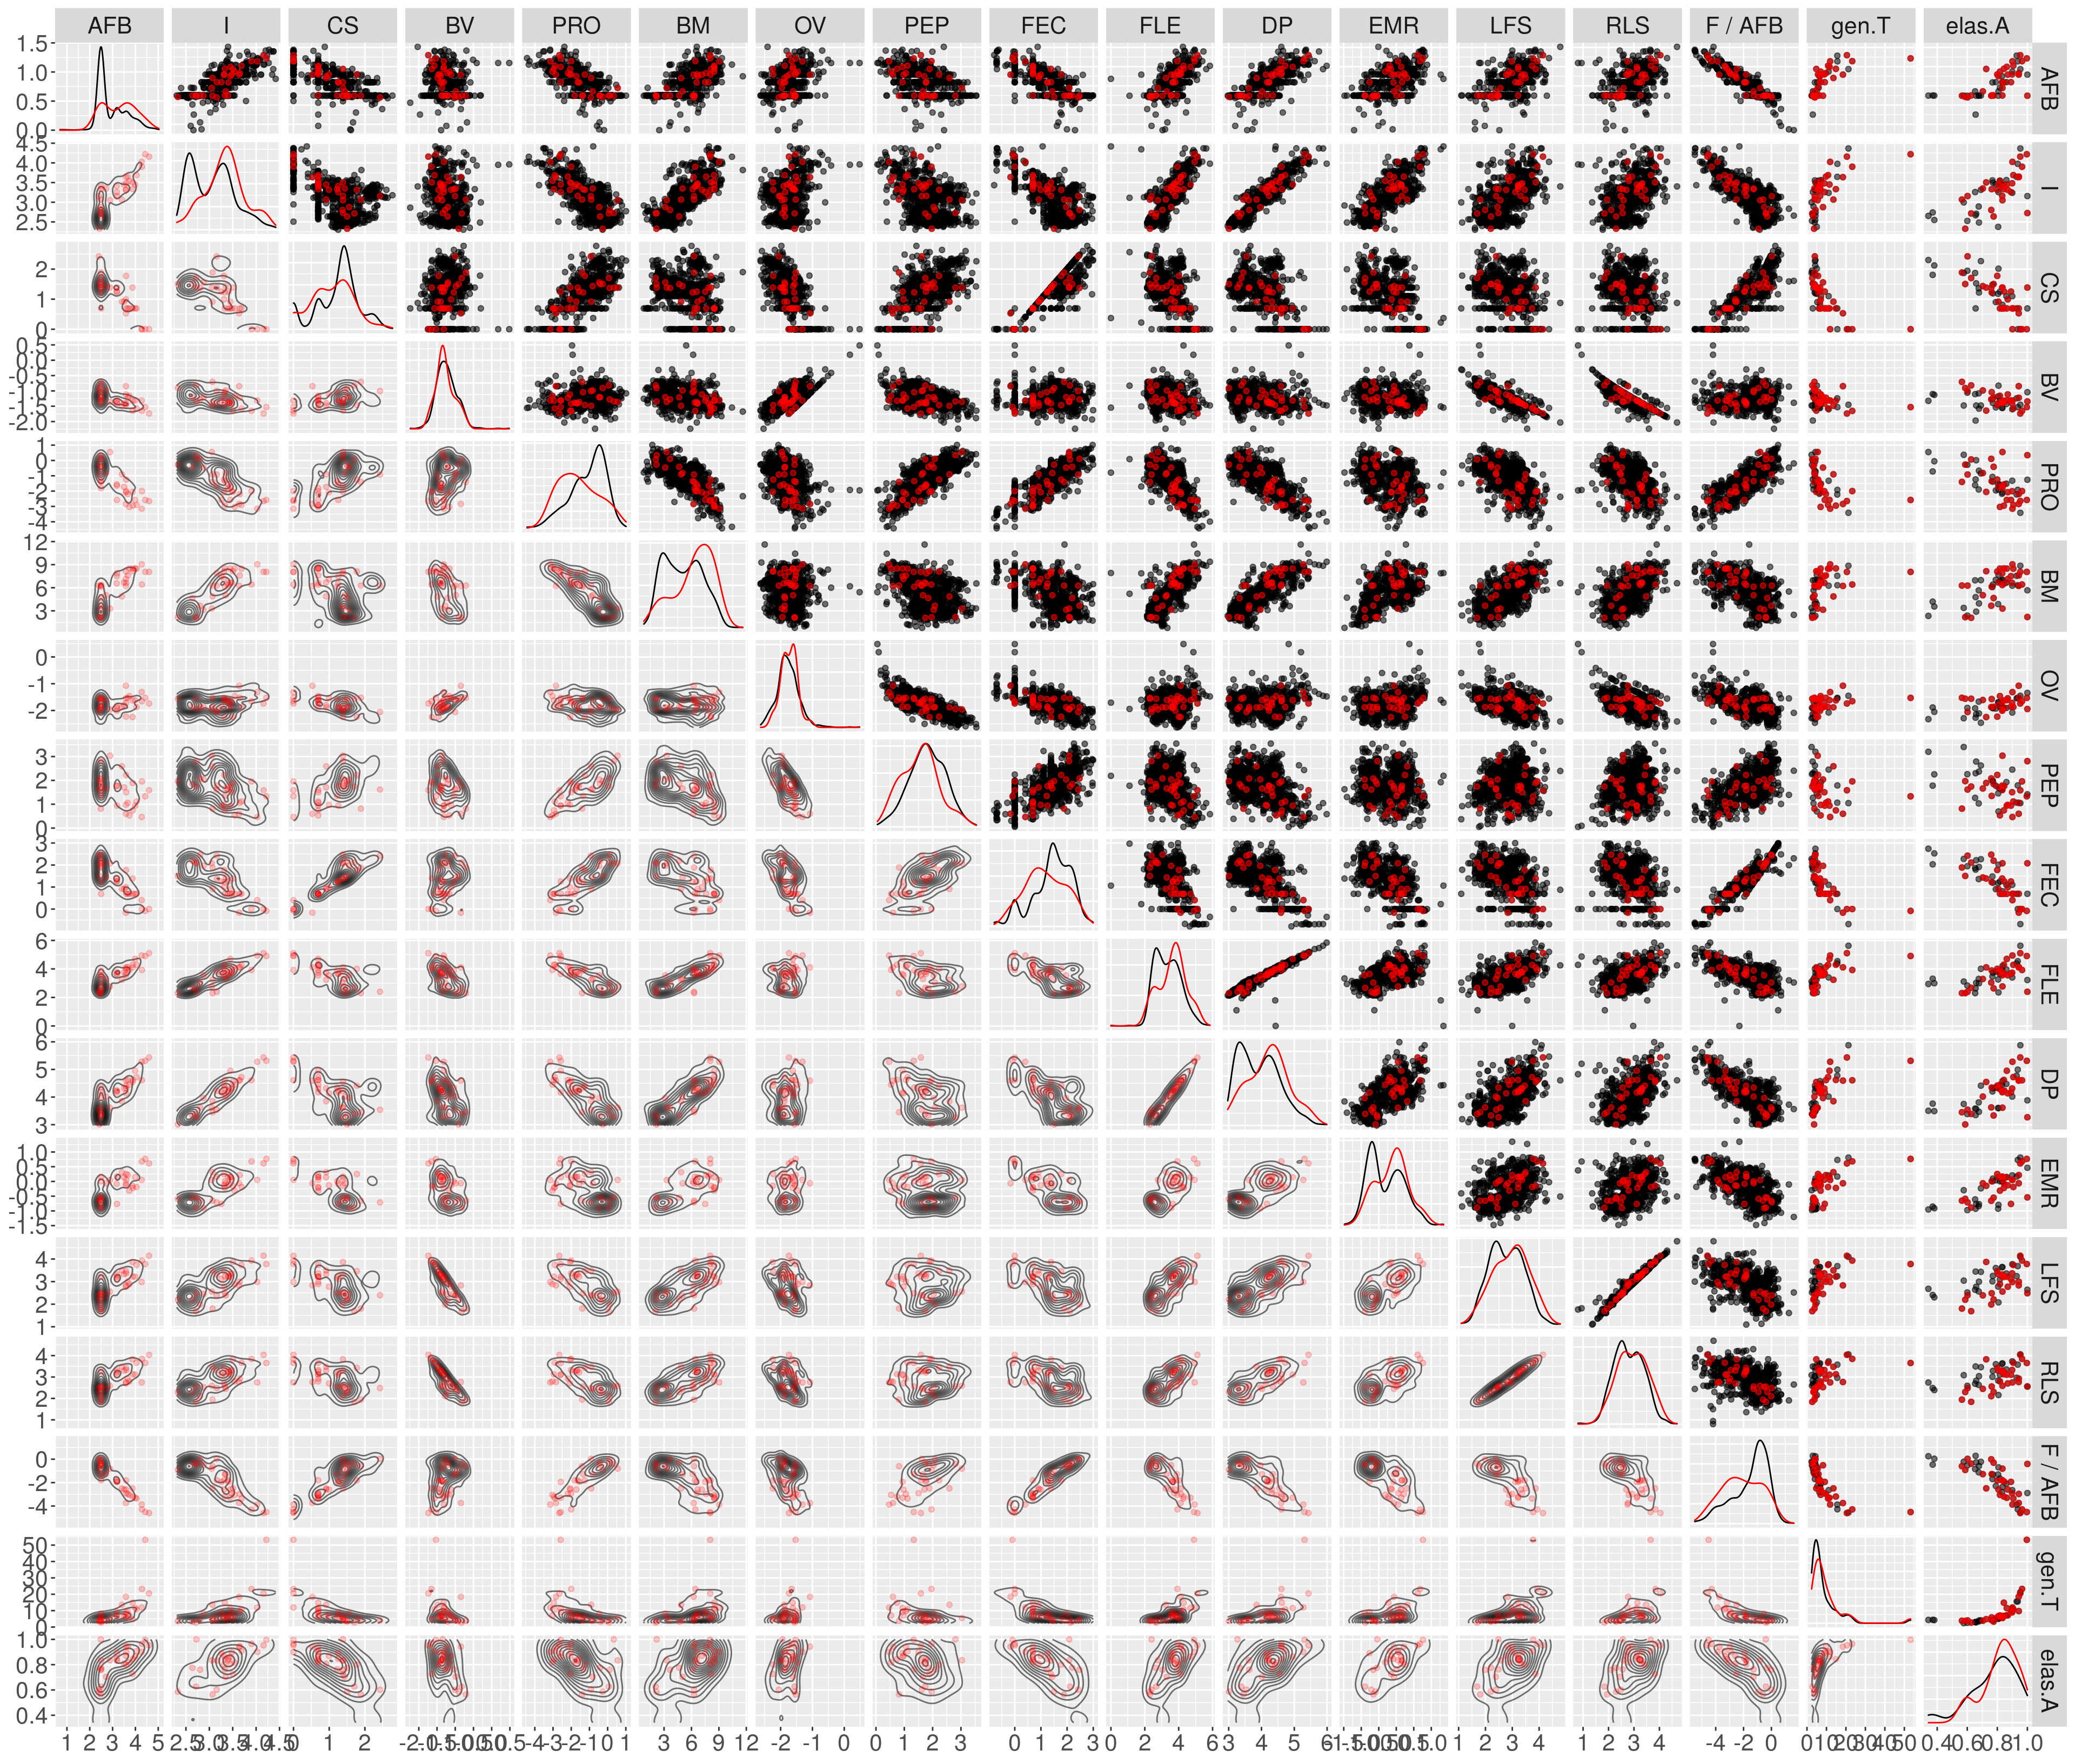
\includegraphics[width=\textwidth]{./Figures/chapter02/fig1-LH_demo_traits.png}
\caption[Traits distribution]{
Biplots (upper triangle) and density plots (lower triangle) of the traits. 
Black for species with either demographic or traits data and red dots for 
species with both demographic (gen.T for generation time and elas.A for 
elasticities to adult survival) and life history traits data (see table 
\ref{tab:table2.1} for details).}
\label{fig:fig2.1}
\end{figure}

From each population matrix model, we calculated 2 demographic 
traits \citep{Caswell2001,Stubben2007}: generation time and elasticity of the 
adult survival. The elasticity matrices show the proportional effects on 
population growth rate for each demographic trait \citep{deKroon2000}⁠. We 
selected elasticities for adult survival and net fecundity as a measure of the 
importance of these components on the life history strategies. However, both 
elasticities were perfectly correlated (correlation coefficient = 1) and we only 
used the elasticities of the adult survival.

To assess how well life history traits correlate with the estimated demographic 
traits, we used the 14 life history traits previously described (Table 
\ref{tab:table2.1}), which were available for the 30 species. The estimated 
elasticities and generation times were modelled as a function of life history 
traits by means of phylogenetic least square regressions (with Pagel’s 
$\lambda$ estimated by means of maximum likelihood), as implemented in the R 
package “phylolm” \citep{Ho2014}⁠. The traits were tested alone and combined 
with other traits by means of phylogenetic principal component analysis 
(PPCA), with maximum likelihood estimates of $\lambda$, as implemented in 
“phytools” \citep{Revell2009a}⁠. The phylogenetic analyses were run with 
2 consensus trees from \citet{Jetz2012}, one for the Ericsson and 
one for the Hackett backbones.
The PPCAs were obtained using the restricted life history dataset (n = 797). We 
assembled all combinations of traits with the only rule that a PPCA should 
include at least a trait related to adult quality, juvenile quality and the 
number of offspring. A total of 10080 combinations of traits were used in the 
PPCAs, from which 2464 were discarded due to unsatisfactory convergence, 
resulting in 7616 trait combinations with a proper PPCA. For each PPCA, we 
selected the Principal Component (PC) that better match the demographic traits 
($\Delta AIC = 0$) and flipped the axis when 
needed, multiplying the PC scores and loadings by -1 in order to sort the 
species from fast (negative values) to slow (positive values).

From all the studied traits, whether alone or combined in a PC, we 
considered those that better explain variation in elasticities or generation 
time as corresponding to the fast-slow axis. We tested their relative 
importance by estimating the AIC based weight of each regression, considering 
the best models as those with 2 units difference from the model with the lowest 
AIC ($\Delta AIC < 2$).


\subsection*{Defining species position on the FS}

Our previous analyses are based on the combination of detailed demographic data 
and full life history information for 30 species. If there are combinations of 
life history traits that accurately predicts variation in elasticities and/or 
generation time, it is possible to use the life history information to assess 
the position in the fast-slow continuum for species for which demographic data 
was unavailable. We defined the position of the species in the fast-slow axis 
as the mean scores of the PCs weighted by the AIC based weights 
of the elasticity models (FSe) and generation time models (FSgt). We did the 
same using all selected PCs and using only the PCs of the best models only 
($\Delta AIC < 2$).

Our finding that to accurately predict elasticities and/or generation time you 
only need a few life history traits, not all of them, open the possibility to 
assess the position in the fast-slow continuum for many more species than those 
with full information on the 14 key life history traits. Therefore, we repeated 
each of the PPCAs identified as best predictors of elasticities and generation 
time in the previous analyses, but now including all the species for which 
information on the underlying life history traits was available, regardless that 
other traits were missing. As before, we defined their position as the mean 
scores of best PCs weighted by the AIC based weights of the elasticity 
and generation time models (FSe and FSgt).

Our extrapolations to estimate the FS assumes that the studied subsets of 
species are representative of the observed variation in the fast-slow continuum. 
This assumption is supported by two analyses. First, the phylogenetically 
corrected correlation \citep{Revell2009a}⁠ of the relevant PCs estimated with
the demographic, restricted and full life history datasets was
\textgreater{0.99} in all cases.
Second, the mean values of each PC estimated for our subsets of species (i.e.
the demographic and restricted datasets) do not significantly differ from those
expected by randomly sampling the same number of species from the full life
history dataset.


\subsection*{Other axes of life history variation}

We analysed the remaining ~9500 (from 9385 to 9604 depending on the life 
history dataset and phylogeny) significant PCs (eigenvalue \textgreater{1}) not 
selected as components of the FS to explore potentially different axes of 
variation. First, we used the correlation among the scores of the PCs to build 
clusters using different minimum absolute correlations (0.7 – 0.9), discarding 
clusters containing less than 5\% of the PCs and removing duplicated clusters in 
different correlation thresholds. 
For each group, we flip the PCs to align the scores and loadings when needed. 
Every cluster represents a potential axis of life history variation. We grouped 
clusters with a correlation on averaged loadings \textgreater{0.95} for 
visualization purposes.


\subsection*{Characterisation of the life history axes}

For each potential axis, we calculated the mean and the standard deviation of 
the loadings multiplied by the relative frequency of the traits. As the 
frequencies of the traits were not the same for each cluster, we also estimated 
the relative weight of each trait as the proportion of the absolute values of 
the loadings in a PC minus the relative frequency of the traits in the PC 
cluster. The relative weight of the traits ranges from -1 to 1, where negative 
values means that the absolute value of the trait loadings are lower than 
expected by the frequency of the trait and positive values for traits with 
higher loadings than expected by the frequency of the trait. In addition, we 
calculated the part of the variance explained by each PC from the total variance 
of the traits included in the PPCA.
For the FS axes we weighted the former metrics by the AIC based weight from all 
the models and also including only the best models.

For each defined axis, we averaged the scores of the species to generate a data 
base of life history for birds. Again, for the FS axes we weighted the PCs 
scores by the AIC based weight for all models and also using the PCs in the 
best models only. The averaged FS scores where then used to predict adult 
elasticities and generation time to compare the performance against the scores 
of single PCs.


\section{Results}

The observed hypervolume based on the 9 non-redundant life history traits is 
much smaller than the hypervolumes predicted by the null models (p-value = 
0.001, see table \ref{tab:tabApp2.1.1}). The closest null model, 
$hv_{nm4}$, is the one that imposes a correlation among traits as observed but 
still 7 times larger than the hypervolume of the observed data. The smaller 
size and aggregation in the hypervolume indicate that not all trait 
combinations are possible, consistent with the existence of constrains and 
trade-offs in the life history evolution. The observed aggregation of species 
is greater for the observed traits than the expected for each $hv_{nm}$
\ref{tab:tabApp2.1.2}. Thus, the existing diversity of life history strategies
seems restricted to certain combinations of correlated traits and shows a
greater concentration in the trait space than expected under multivariate
normality.

From the 7631 trait combinations, including single traits, the selected PCs 
scores from the PPCAs combining sets of traits, and other metrics used to 
describe the fast-slow continuum in the literature, 104 where among 
the ones that better predict elasticities for adult survival ($\Delta AIC < 2$),
while for predicting generation time 468 trait combinations where among the
bests (see \href{TODO}{FS\_modelSelection.xlsx in the ESM}). All the best
%TODO: add url to ESM
predictors are PCs scores except for the single trait clutch size that is also
part of the best predictors for the elasticity of the adult survival.
The best PCs come from PPCA with $5.9 \pm 1.3$ combined traits for adult 
survival elasticities and $6.2 \pm 1.3$ for generation time. The variance 
explained by the PCs account for $54\% \pm 0.008$ of the variance of the traits 
sets selected for the elasticities of adult survival and $48\% \pm 0.008$ 
for the trait sets selected for generation time. Here we report the results for 
the restricted life history dataset using the phylogeny based on the Hackett 
backbone, see \ref{ch:Appendix2.1} for the details of the extended life 
% TODO: check appendix and ESM references and define tables
%   check vignette for tables or boxplots
history dataset and the phylogeny based on the Ericson backbone.

Although single traits are often used as surrogate for the FS, no single 
trait appears among the best models for neither elasticity nor generation time 
(Supplementary table S3). The ratio FEC / AFB, which has also been suggested to 
accurately describe the FS \citep{Oli2004}⁠, is not among the best traits, 
alone or in combination, that better explains adult survival elasticities 
($\Delta$AIC = 85.6) nor generation time ($\Delta$AIC = 10.2). 

\begin{figure}
\centering
\includegraphics[width=\textwidth]{./Figures/chapter02/fig2-FSaxes.png}
\caption[Fast-Slow PC loadings]{
Importance of the traits describing the fast-slow continuum. Top panel: Loadings 
mean $\pm$ SD of the selected PCs combining sets of life history traits that 
better describe the fast-slow axis. Bottom panel: Relative weight of the life 
history traits in the fast-slow continuum. Values range from -1 to 1, where 
negative values means that the absolute value of the trait loadings are lower 
than expected by the frequency of the trait and positive values for traits with 
higher loadings than expected by the frequency of the trait in the selected 
PCA (see main text for details). The loadings and frequencies com from 
selected PCs that better predict elasticities of the adult survival or 
generation time, weighted by the AIC based weight of the models taking all or 
only the models with $\Delta AIC < 2$ (best AIC).}
\label{fig:fig2.2}
\end{figure}


Figure \ref{fig:fig2.2} shows the loadings of each life history trait in the 
best
FS axes, for both elasticities and generation time. In both cases, the life 
history traits with higher and consistent weights include CS and AFB. 
However, there are two main differences. First, incubation period is more 
influential for the axis based on generation time than for those based on 
elasticities. Second, FEC seems more important for PCs selected to 
predict generation time. Other traits in selected PCs have huge variability 
(see SD bars in figure \ref{fig:fig2.2} and depends on whether all models or 
only the best ones ($\Delta AIC < 2$) are used to weight the PC. Other traits 
commonly included in the fast-slow axis such as LFS or BM seems unrelated to 
the demographically defined fast-slow axis defined by our methodology.

One advantage of combining all PPCA in single weighted-average axes is that it 
allows estimating the position of a species in the FS even when some scores 
cannot be estimated due to missing data for life history traits combined in a 
PPCA. We thus estimated the fast-slow continuum for up to 1516 species for each 
respective axis. The two 
estimated FS axes (FSe and FSgt) are highly correlated with each other 
(Phylogenetic correlation =  0.85 and 0.74 for all or best models 
only, n = 797 species), are only weakly correlated 
with body mass (Phylogenetic correlations = 0.5 and 0.34, respectively) and 
exhibits substantial phylogenetic effects ($\lambda > 0.95$).

\begin{figure}
\centering
\includegraphics[width=\textwidth]{./Figures/chapter02/fig3-Secondary axes.png}
\caption[Alternative axes groups and PC loadings]{
Importance of the traits for clusters of similar significant PCs not present in 
the FS axes. Each group contains PCs with scores correlation greater than the 
correlation specified in the group name in the inset dendogram (e.g. grCor0.8 
means correlation \textgreater{0.8}). Top panel: Loadings mean $\pm$ SD for the 
traits of each group of PCs. Bottom panel: Relative weight of the life history
for each group of PCs (see figure \ref{fig:fig2.2} for details).}
\label{fig:fig2.3}
\end{figure}

Although the PCs representing fast-slow continuum explains around 50\% of the 
variation in life history traits, much variation still remains to be explained.
To explore thus variation, we extracted all the PCs with Eigenvalue
\textgreater{1} among the
%TODO: cite Kaiser criterion (Legendre P, Legendre L (2012) Numerical Ecology 
% (Elsevier, London), 3rd Ed, p 1006)
PCs not selected as descriptors of the Fast-slow continuum, and classified them 
in eight groups based on a cluster analyses of species scores (fig.
\ref{fig:fig2.3}). These clusters classify together PCs that represent similar
life history axes, which may then be interpreted by examining their traits
loadings. The averaged loadings of these groups suggest at least three axes of
life history variation that are independent of the fast-slow continuum.
The most important one in terms of variance explained is the degree of
iteroparity (grCor0.75\_18, grCor0.7\_43 and grCor0.75\_29 in figure
\ref{fig:fig2.3}), quantified as the brood value index \citep{Bokony2009}⁠,
which represents whether all reproductive effort is allocated into a few
reproductive events (i.e. high brood value as each brood has high contribution
to fitness) or instead the effort is distributed into many attempts (low brood
value), whether in a same breeding season or in different ones. Most of the
species in ourdataset only breed once per year, therefore the brood value is
highly correlatedwith the RLS and LFS and it often appears loading together on
the same PC.
Another life history axis that appears consistently in the analyses is related 
to the offspring quality-quantity trade-off (grCor0.8\_24, grCor0.7\_17 and 
grCor0.75\_19 in figure \ref{fig:fig2.3}), with species laying few eggs yet
relatively large at one extreme and species laying many eggs of small size at
the other extreme. The 4th axes, grCor0.8\_5 in \ref{fig:fig2.3} is related to
PEP, PRO and FEC and reflect the productivity of the species in terms of
investment in reproduction. This axis is correlated with FSgt (-0.73).

% TODO: phylogenetic signal
Scores for all described axes are available in the ESM. % TODO: add URL


\section{Discussion}

Our finding that not all combinations of life history traits are possible is at 
first sight unsurprising, given the existence of overwhelming evidence of life 
history trade-offs and constraints. Demonstrating it is however important 
because our empirical evidence is based on an unusually large and representative 
sample of species. We therefore can largely exclude the possibility that the 
observed pattern results from sampling biases.

The Fast-Slow continuum emerged as a major axis structuring life history 
variation in birds, confirming and generalising previous studies. Our 
empirically-derived estimates of the fast-slow continuum reflect well the 
fecundity-survival trade-off, are strongly correlated among each other and are 
largely independent of body size. Although a variety of life history traits 
contribute to define the continuum, FEC and AFB appear particularly relevant in
line with some previous suggestions. However, these life history traits are not
good surrogates of the continuum when alone, but only when combined with other
life history traits.

Most life history traits show a strong allometric relationship with adult body 
mass, in part reflecting constrains associated with scaling laws. For example, 
the higher metabolic rate of smaller animals may allow them to produce offspring 
faster. However, body size may also play part of the fast-slow continuum through 
its effect on age-specific mortality, if for example a large body reduces 
predation risk. Our analyses support this line of thinking, showing that body 
size is selected in some (but not all) of the models that best predict 
elasticities of adult survival although always in combination with other life 
history traits.

Although the fast-slow continuum is widely considered the most important axis of 
life history variation, growing evidence suggest the existence of other relevant 
axes. By accurately quantifying the fast-slow continuum, we could investigate 
the remaining axes of life history variation.
Our analyses identified an important axis of variation related to the timing of
reproductive bouts. This axis, the so-called brood value \citep{Bokony2009} or
semelparity-iteroparity \citep{Gaillard1989}, represents the extent to which
all reproductive effort is allocated into a few reproductive events (i.e. high
brood value) or instead the effort is distributed into many attempts (low brood
value), whether in a same breeding season or in different ones. Most of the
species in our dataset only breed once per year, therefore the brood value is
highly correlated with the reproductive lifespan and it often appears loading
together on the same PC. However, a low brood value may also be achieved by
reproducing multiple times during a same breeding season, a strategy that is
used by some pigeons and starlings.

Other previously suggested life history axes that appear consistently
once the fast-slow continuum is factored out are related to the duration of the
development and the trade-off between offspring quantity and quality
\citep{Promislow1990,Bielby2007,Dobson2007}.

Much of the ecological relevance of the fast-slow continuum resides in its 
influence on population dynamics under challenging conditions, an issue 
particularly relevant in the current context of global environmental change. 
Species at the fast extreme have a higher potential to rapid population grow 
than those at the slow extreme, which may facilitate recovering from a 
population crash. When population size is low, however, they also tend to be 
more susceptible to populations fluctuations associated with demographic 
stochasticity. The relevance of these mechanisms can only be investigated by 
properly defining and accurately quantifying the fast-slow continuum based on 
the entire life cycle. 

Moreover, the influence of other life history axes needs also to be considered. 
A low brood value has been suggested to favour geometric population growth under 
environmental stochasticity through mechanisms such as bet-hedging 
\citep{Stearns2000a}⁠ and the storage effect \citep{Cubaynes2011}. The finding
that brood value and the fast-slow continuum are different life history axes but
share critical life history traits opens the possibility to life history
strategies that facilitate a rapid population growth when conditions are
favourable and reduce the costs of a reproductive failure when conditions are
unfavourable. For example, brood value seems a significant trait to adapt to
new environments in introduced species or species colonising urban habitats
\citep{Sol2012a,Sol2014}.

Despite having solid foundations, life history theory has surprisingly achieved 
little success in predicting the response of organisms to rapid human-induced 
environmental alterations such as habitat loss, climate change and biological 
invasions. This is paradoxical considering that some proposed mechanisms were 
proposed more than 50 years ago. A more integrative and mechanistic view of life 
history variation can contribute to develop a more predictive body of theory 
regarding how life history and the possible interactions with behaviour
\citep{Ricklefs2002,Reale2010a,Sol2018,Maspons2019} affects the response to
environmental changes. The provided axes of life history variation can open
further studies to elucidate the links between environmental condition and the
evolution of life history strategies.

\section*{Electronic Suplementary Material}

Electronic supplementary material is available online at
\url{https://github.com/jmaspons/Thesis/...} % TODO: upload and link

%************************************************
\chapter[Behaviour and life history in novel environments]{Behaviour, life
history and persistence in novel environments
  \footnote{Published in: Maspons, J., R. Molowny‐Horas, \& D. Sol. 2019. Behaviour, life
  history and persistence in novel environments. \textit{Phyl. Trans. R. Soc. B}
  374:20180056.
  \href{http://dx.doi.org/10.1098/rstb.2018.0056}{doi:10.1098/rstb.2018.0056}
  }
}\label{ch:LH-Behaviour model}
%************************************************


\section*{Abstract}

Understanding what affects population growth in novel environments is
fundamental to forecast organisms’ responses to global change, including
biological invasions and land use intensification. Novel environments are
challenging because they can cause maladaptation, increasing the risk of
extinction by negative population growth. Animals can avoid extinction by
improving the phenotype–environment match through behavioural
responses, notably matching habitat choice and learning. However, the 
demographic consequences of these responses remain insufficiently understood in
part because they have not been analysed within a life-history context. By
means of an individual-based model, we show here that matching habitat
choice and learning interact with life history to influence persistence in
novel environments. In maladaptive contexts, the likelihood of persisting is
higher for life-history strategies that increase the value of adults over the
value of offspring, even at the cost of decreasing reproduction. Such a strategy
facilitates persistence in novel environments by reducing the costs of a 
reproductive failure while increasing the benefits of behavioural responses. Our
results reinforce the view that a more predictive theory for extinction risk
under rapid environmental changes requires considering behavioural
responses and life history as part of a common adaptive strategy to cope
with environmental changes.
This article is part of the theme issue ``Linking behaviour to dynamics of
populations and communities: application of novel approaches in behavioural
ecology to conservation''.

\bigskip
\textbf{Keywords:} Biological invasions, Extinction risk, Demographic
stochasticity, Cognitive ecology, Habitat selection, Urbanization

\clearpage


\section{Introduction}

Most organisms experience serious difficulties when exposed to novel
environments. Novel contexts often generate mismatches between the phenotype and
the environment, leading to maladaptation and extinction through negative
population growth \citep{Bell2017}. Maladaptation is one of the reasons why translocations
of species from their native ranges to novel environments generally fail to establish
self-sustaining populations \citep{Sol2016, Sakai2001a}, and it is also a primary cause of extinction by
land use intensification \citep{Sih2011}. Given that biotic exchanges and land use
intensification are becoming increasingly frequent as a result of human activities, there is an
urgent need to understand the mechanisms that influence population persistence
in novel environments.

Several processes can allow organisms to improve the matching of their
phenotypes to new contexts and hence facilitate persistence in novel environments.
Natural selection—the most obvious process—can contribute to
reconstitute the phenotype–environment match through genetic changes, a process
known as evolutionary rescue \citep{Bell2017}. However, an evolutionary rescue is less
effective in animals with long generation time, such as many birds and mammals,
which exhibit slow evolutionary responses to selection. In these animals, behavioural
responses are an alternative to reduce the phenotype–environment
mismatch \citep{Sih2011, Klopfer1981, Sol2003a, Tuomainen2011, Kokko2001}. Individuals may, for instance, improve fitness in novel environments
by choosing the habitats where they live and reproduce that best fit their
phenotype, a process known as matching habitat choice \citep{Nicolaus2018, Stamps2007, Greene2001, Schmidt2010}. Animals can
also decide when is best to reproduce, and skip reproduction
when conditions are unfavourable \citep{williams1966adaptation}.

The choice of where and when to live and reproduce can
express activational plasticity, that is, an innate response to
environmental cues \citep{Snell-Rood2013, Sol2013a}. In a novel environment, however,
individuals must often take decisions with insufficient information
and using cues that may have changed relative to
those from the old environment, which can lead them
to settle in poor-quality habitats (ecological traps) \citep{Kokko2001}. Yet,
animals can improve decision-making, and hence avoid
extinction, through learning \citep{Grieco2002, Kawecki2010}. Learning can modify
decision-making based on previous experiences of the individual \citep{Baudains2007, Eliassen2007}
—for example, changing habitat after a
reproductive failure—or by using public information generated
by more experienced conspecific or heterospecifics
\citep{Doligez2002}. Evidence is accumulating that species which readily
adjust behaviours to novel contexts are better able to survive
and reproduce in a novel environment than species that
persist with the behaviours of their old environments \cite{Kawecki2010, Dukas2008}.

While the importance of behaviour in the response to
environmental changes is widely recognized, we still lack a
general theory regarding how such processes influence
population growth in novel environments \citep{Sol2016}. One important
reason is that behavioural responses have rarely been
investigated within a life-history context \citep{Sol2016, Ricklefs2004}. Life
history—defined as the way organisms distribute their limited
time and energy into growth, reproduction and
survival \cite{stearns1992evolution}—is relevant because it affects how populations
increase and fluctuate over time. The demography of the
organism is particularly influenced by its position in the
fast–slow continuum of life-history variation \cite{Stearns1983a}. Species
at the fast side of the continuum have short life expectancy
but mature early and show high fecundity, which give
them a high potential for rapid population growth under
favourable conditions. Growing fast may confer advantages
during the invasion of novel environments by reducing the
period that the population remains small and hence vulnerable
to extinction by demographic stochasticity. Species at
the slow side of the continuum have delayed maturity and
low fecundity, and hence cannot increase in number so fast
when the population is small. Yet, their long life expectancy
(and long generation time) buffers their populations from
fluctuations driven by demographic and environmental stochasticity
that can lead to extinction \cite{Saether2013, Saether2004}. A slow strategy
also reduces the fitness costs of a reproductive failure, as individuals
have higher chances of breeding again in the future.
This offers advantages in novel environments by spreading
the risk of reproductive failure over several breeding attempts
(a type of bet-hedging) and by allowing individuals to skip a
reproductive event (and hence improve their survival) when
conditions are unfavourable \cite{Sol2012a}.

Thus, when we analyse how behavioural responses affect
the demography of animals in novel, stochastic environments,
we need to be aware that these responses will be affected by the
organism’s life history. This is relevant because the position of
the animal in the fast–slow continuum can alter the benefits
and costs of gathering environmental information and constructing
appropriate behavioural responses \cite{Forcada2008, Saether2000,
Lewontin1969, Saether2005a, Starrfelt2012}. The net
benefit should generally be higher in slow animals, which are
less constrained by time to explore and learn, and can use the
learned behaviours for longer periods. The costs of delaying
reproduction when conditions are unfavourable should also
decrease in slow species, as individuals can reproduce again
in the future, increasing the opportunities for acquiring
environmental information and, through learning, improve
the match of the phenotype to the novel conditions \cite{Sol2012a}.
The demographic consequences of behavioural responses in
novel, stochastic environments are also expected to vary
depending on whether the phenotype–environment mismatch
mainly affects offspring or adult survival. This is because fast
and slow strategies differ in their sensitivity to changes in the
demographic parameters, with fast strategies being highly
sensitive to changes in fecundity and slow strategies to changes
in adult survival \cite{Gaillard2000a}. Thus, understanding how behavioural
responses contribute to population persistence in novel, stochastic
environments requires us to consider the position of
the animal in the fast–slow continuum \citep{Sol2016}.

While the demographic consequences of behaviour have
been previously modelled by several authors \citep{Kokko2001, Cressman2013, Kisdi2002,
kawecki1995demography, Strasser2012}, it
remains to be seen to what extent behavioural responses influence
population growth in novel, stochastic environments as a
function of the position of the animal in the fast–slow continuum.
Here, we use an individual-based simulation model
to address this issue. The behavioural responses that we investigate
include innate preferences for habitats that better
matches the organism’s phenotype, learning rules to reduce
the preference for inadequate habitats and decisions about
skipping a reproductive event when individuals stay in a habitat
that does not match their phenotype. We use the model to
illustrate how considering life-history variation refines predictions
of classic theory regarding the role of behaviour in
facilitating population persistence in novel environments.


\section{Model description}

Building on previous studies \citep{Cressman2013, kawecki1995demography}, we envision a species
that is introduced in a novel region with two habitats.
Individuals are allowed to survive, reproduce and move
between habitats, and the likelihood that the population persists
in the novel region (establishment success) is estimated
through simulations (electronic supplementary material,
figure \ref{fig:figApp3.2.1}). Establishment success is estimated through a
stage-structured population-based model (which allows us
to compare the outcome for species differing in life history),
in scenarios varying in the degree of phenotype–environment
mismatch (causing negative population growth) and
demographic stochasticity (causing extinction by demographic
accidents). The introduced species has a particular
life-history strategy that positions it along the fast–slow continuum,
fixing the values of its onset of first reproduction,
average fecundity and age-specific survival of individuals
(see details below). Behavioural responses are studied by
assessing how modifying the probabilities of changing habitat
and skipping reproduction affects establishment success.
Below, we briefly summarize the main features of the
model. For further details about specific parts of the model
and about its inner workings, we refer the reader to the electronic
supplementary material. The model was built using
the R language \citep{RCoreTeam}, and an accompanying R package implementing
the model, with its corresponding tutorial, is also
offered as the electronic supplementary material at
\url{https://dx.doi.org/10.6084/m9.figshare.c.4546955}.


\subsection*{a) Stage-classified population}

We chose a stage-classification approach to account for the
complex life cycle of our simulated populations. Based on
pre-breeding census, we classify the population into three individual
classes: juveniles, subadults (only for strategies with age
at first reproduction greater than 1 year) and adults. In turn,
adults are divided into non-breeder (i.e. adults that decide
not to breed in a given year) and breeders. Finally, breeding
individuals are split at each brooding step into successful or
failed breeders, distinguishing whether breeding yields viable
juveniles or not, respectively. Only females are considered.


\subsection*{b) Demographic model set-up}

Our population model includes the main processes that must be
considered when evaluating the life cycle of a stage-classified
population, namely survival, growth and reproduction (table \ref{tab:table3.1}):
\begin{description}
  \item[(i) survival:] each stage-class ( juveniles, subadults, non-breeding
    adults and breeding adults) is defined by an annual
    survival rate. In addition, juvenile survival is decomposed
    into individual survival and brood survival, the latter
    affecting all individuals in the same brood (e.g. as a
    result of nest predation). Data about the sources of juvenile
    mortality are scarce, and hence, we fixed the brood level
    mortality to account for 50\% of the juvenile mortality;
  \item[(ii) growth:] individuals can be promoted to the next stage if
    they survive to the next year. Individuals only remain
    1 year in the juvenile class, after which they move up
    to the subadult or adult class. After they reach adulthood,
    they remain in that condition until they die; and
  \item[(iii) reproduction:] each year, the algorithm determines
    which proportion of adults becomes non-breeders or
    breeders, and also which proportion of the latter
    may successfully breed. Only adults that are classified
    at each step as breeders can reproduce during a year.
\end{description}


\begin{table}
\caption[Notation]{Notation followed to describe the stochastic population model.}\label{tab:table3.1}
\begin{tabular}[b]{@{}p{1.5cm}p{13cm}@{}}
\toprule
\textbf{Symbol} & \textbf{Definition}                                                                                                                                                                                                                                                                                        \\ \midrule
$q$   & Number of offsprings per brood in habitat $h$                                                                                                                                                                                                                                                                        \\
$m$   & Number of broods per year                                                                                                                                                                                                                                                                                            \\
${n}_{Sa}$        & Number of sub-adult stages                                                                                                                                                                                                                                                                               \\
$x$   & Labels for adult breeder type, $x= \{nb, b, b_{s}, b_{f}\}$. Label $nb$ identifies adults that skip breeding and label $b$ indicates adult individuals that try to breed. In turn, the latter can be divided into those which breed successfully (labelled $b_{s}$) or those which fail to do so (labelled $b_{f}$)  \\
$y$   & Labels for survival, $y= \{j, sa, nb, b\}$, where labels refer to juveniles, subadults, non-breeder and breeder adults, respectively                                                                                                                                                                                 \\
$h$   & Index for habitat type, $h= \{1, 2\}$                                                                                                                                                                                                                                                                                \\
$r$   & Label for subadult stage, $r= \{r_{1} \cdots r_{n_{Sa}}\}$                                                                                                                                                                                                                                                           \\
$t$   & Subindex for time steps, measured in years, $t= \{1 \cdots 50\}$                                                                                                                                                                                                                                                     \\
${p}_{h}^{b}$     & Probability for an individual to become a breeder (successful or not) in habitat $h$                                                                                                                                                                                                                     \\
${p}_{h}^{b_{f}}$ & Probability of complete brood failure for a breeder in habitat $h$                                                                                                                                                                                                                                       \\
${p}_{h,S_{x}}$   & Probability of survival in habitat $h$ for individuals $x$                                                                                                                                                                                                                                               \\
$p_{h, s_{y}}$    & Probability of survival in habitat $h$ for individuals of type $S_{y}$                                                                                                                                                                                                                                   \\
\noalign{\bigskip}
${p}_{1\rightarrow2}^{x}$ \\ ${p}_{2\rightarrow1}^{x}$ & Probability for an adult to move from habitat type 1 to 2, or vice versa                                                                                                                                                                                            \\
\noalign{\bigskip}
${p}_{1\rightarrow2}^{r}$ \\ ${p}_{2\rightarrow1}^{r}$ & Probability for a stage-r subadult to move from habitat type 1 to 2, or vice versa                                                                                                                                                                                  \\ \bottomrule
\end{tabular}
\end{table}



\subsection*{c) Implementation of the demographic model}

Each simulation starts with the introduction of a particular
number of adults with an evolved life-history strategy along
the fast–slow continuum. This cohort of adults is equally
distributed between both habitats (labelled $h$). After the
introduction phase, the growth of the population from year $t$
to $t + 1$ is determined by the number of births and deaths
within each habitat. The cohort of adults in each habitat is
first divided into non-breeder and breeder adults with a probability
$p^{b}_{h}$. Then the model enters the breeding phase, which
consists of a loop within which m breeding episodes take
place. At each step within that loop, breeder adults are randomly
split between failed and successful breeders ($p^{b_{f}}_{h}$), and
only the latter give rise to viable juveniles. The number of juveniles
per successful breeding attempt is the product of the clutch
size ($q$) and probability for a juvenile to survive ($p_{h,S_{j}}$). After each
reproductive event, breeders (failed or successful) may change
habitat with a probability $p^{x}_{1\rightarrow2}$ (if they move from habitat 1 to
habitat 2) or $p^{x}_{2\rightarrow1}$ (if they move from habitat 2 to habitat 1),
with $p^{x}_{1 \rightarrow 2} = 1 - p^{x}_{2 \rightarrow 1}$. Once the breeding loop has finished,
non-breeder adults and subadults are allowed to change habitats
and, finally, all individuals are promoted to the next class
after their survival is evaluated (table \ref{tab:table3.1}).


\subsection*{d) Demographic stochasticity}

Demographic stochasticity is implemented both in the survival
probability of each age class and in the probability of a brood
failure (table \ref{tab:table3.1}) by means of binomial distributions defined
by each probability and population size, obtaining random
deviates from the mean value. The number of individuals
introduced defines the extent to which the population is
exposed to demographic stochasticity. We consider population
growth to be density-independent (i.e. we assume that during
the establishment phase, the population is far from its carrying
capacity) and little influenced by Allee effects \citep{kawecki1995demography}.


\subsection*{e) Environmental scenarios to simulate maladaptation}

The degree of match between the phenotype and the environment
is modelled by varying the costs of selecting a habitat
where the species can be viable but maladapted \citep{Kisdi2002}, defined
by the following scenarios:
\begin{description}
  \item[(i) high phenotype–environment match], simulated by defining
    the two habitats as identical and without penalties
    (scenario 1). Therefore, fecundity and survival rates
    attain their maximum values, as defined by the species’
    life history;
  \item[(ii) insufficient phenotype–environment match penalizing adult
    survival] ($p_{h,s_{x}}$), simulated by imposing an increase in
    adult mortality of either 50\% (scenario 2.1) or 100\% (scenario
    2.2) in habitat 2 (low-quality habitat, hereafter); and
  \item[(iii) insufficient phenotype–environment match penalizing offspring
    survival], simulated by increasing the probability
    of a brood failure ($p^{b_{f}}_{h}$) by either 50\% (scenario 3.1) or
    h100\% (scenario 3.2) in habitat 2 (low-quality habitat).
\end{description}


\subsection*{f) Behavioural responses}

To investigate how behavioural responses influence persistence
in the different environmental scenarios, we first explore
what happens when individuals are not allowed to take
decisions (i.e. their behaviour is ‘neutral’). Thus, we assume
that the probability of changing from one habitat to the other
is the same ($p^{x}_{1 \rightarrow 2}$ and $p^{x}_{2 \rightarrow1} = 0.25$) and all individuals reproduce
after achieving adulthood ($p^{b}_{h} = 1$). To incorporate
behavioural responses, we modify these parameters as follows:
\begin{description}
  \item[(i) matching habitat choice] (abbreviated \textit{GoodChoice}) is an
    innate preference for the habitat that better matches
    the organism’s phenotype (i.e. the high-quality habitat),
    which reduces either adult or offspring mortality
    depending on the environmental scenarios previously
    defined. To do so, the preference for habitat 1 is either
    doubled (moderate response) or quadrupled (strong
    response) in each simulation;
  \item[(ii) habitat mismatching choice (WrongChoice)] describes an
    innate preference for the habitat that does not match
    the organism’s phenotype (low-quality habitat), thereby
    increasing either adult or offspring mortality depending
    on the environmental scenario. Habitat mismatching
    choice simulates ecological traps \citep{Kokko2001}. To do so, $p^{x}_{1 \rightarrow 2}$ is
    either doubled (moderate response) or quadrupled
    (strong response) in each simulation;
  \item[(iii) reproductive skipping (ReprSkip)] refers to the decision
    about skipping or not a reproductive event when the
    individual is in the low-quality habitat. This simulates
    the storage effect \citep{Warner1985a} by which adults improve survival
    by skipping reproduction when conditions are
    inadequate. To achieve it, the probability to breed in
    habitat 2 is reduced to either 0.5 (moderate response)
    or 0.25 (strong response) in each simulation. Non-breeding
    adults are given a 50\% increase relative to breeding
    adults in the probability to survive from $t$ to $t + 1$;
  \item[(iv) learning through exploration (LearnExpl)] refers to a
    decreased preference for the low-quality habitat after
    exploring any of the two habitats. This describes the
    process of gathering information to make more
    informed decisions \citep{Eliassen2009}. To do so, the preference for
    the high-quality habitat once the individual has
    explored the low-quality habitat is either doubled
    (moderate response) or quadrupled in each simulation
    (strong response), while the probability of moving
    from the best to the worse habitat ($p^{x}_{1 \rightarrow 2}$) is set to
    zero, except for breeders that failed to reproduce. In
    this latter case, $p^{b_{f}}_{1 \rightarrow 2}$ is doubled or quadrupled; and
  \item[(v) learning from a breeding experience (LearnBreed)] is the
    decision about changing habitat or not according to
    the result of the past breeding attempt. Regardless of
    the habitat, a reproductive failure in the habitat
    makes it more likely that individuals change the habitat
    in the next breeding attempt. Thus, $p^{x}_{1 \rightarrow 2}$ and $p^{x}_{2 \rightarrow 1}$
    is 0 when the reproduction is successful (i.e. at least
    one offspring is produced), and the probability of
    shifting habitat in each simulation is either doubled
    (moderate response) or quadrupled (strong response)
    after a failed reproduction.
\end{description}


\subsection*{g) Simulations}

The probability of persisting in the novel environment was
estimated for different initial population sizes ($N_{0}$ from 2 to
100) as the proportion of populations that avoid extinction
after 50 years, based on 10 000 replicates. This allowed us to
describe the curves relating the likelihood of establishment
with $N_{0}$ for each possible combination of life-history strategy,
behavioural response and environmental scenario (see details
below). As an integrative measure of the likelihood of population
persistence, we used the initial population size that
allows 50\% of the populations to persist during the 50 years
($N_{0}P_{50\%}$). The value of each $N_{0}P_{50\%}$ was estimated through a
lineal search testing different initial population size.


\subsection*{h) Exploration of the parameters}

The exploration of the parameters was carried out by crossing
all combinations of life-history traits with the behavioural
responses and environmental scenarios. To obtain all
combinations of life-history traits, we first defined regular
sequences for each life-history trait within the ranges found
in birds, based on published information \citep{Sol2012a, Sol2018}. The traits
and ranges included adult survival (0.1–0.95), number of
broods per year (1–2), number of offspring per brood (1–20)
and age at first reproduction (1–4). For subadult stages, we
used the same survival as for the adults. Next, we created all
the possible combinations of life-history traits and fixed the
deterministic growth rate $\lambda$ from 1.05 to 1.2 by adjusting juvenile
mortality rate, solving the Euler–Lotka equation (see the
electronic supplementary material for details). Strategies with
juvenile survival lower than 0.1 or higher than adult survival
were discarded. The total number of life-history strategies
resulting from the combination of life-history traits was 3612.

To evaluate the impact of these life-history strategies on
the persistence of the populations in the novel environment,
we first tested the sensitivity of $N_{0}P_{50\%}$ to $\lambda$, fecundity,
age at first reproduction and age-specific survival by means
of partial rank correlation coefficients (PRCC) \citep{saltelli2004sensitivity}. This
method measures the association between two variables
while accounting for the effect of other variables, and has
the advantage of being little affected by collinearity and
non-linear relationships. In addition, we also compared how
$N_{0}P_{50\%}$ varies between fast and slow strategies as a function
of behavioural responses and maladaptive scenarios. The
position of each life-history strategy along the fast–slow continuum
was assessed as the relative sensitivity (i.e. elasticity)
of population growth to changes in fecundity. Given that
the fast–slow continuum describes a fecundity–survival
trade-off \cite{stearns1992evolution}, any combination of life-history traits characterizing
slow species should be related to high elasticities for
adult survival and low elasticities for fecundity, the contrary
being true for fast species. We classified life-history strategies
as slow when their elasticities for fecundity were in the first
quartile and as fast when their elasticities for fecundity were
in the uppermost quartile (using elasticities for adult survival
gives qualitatively similar results).


\section{Results}

\subsection*{a) Behavioural responses in stochastic, maladaptive scenarios}

\begin{figure}
\centering
\includegraphics[width=\textwidth]{./Figures/chapter03/Fig_1.jpg}
\caption[Persistence as a function of LH, behviour and scenario]{
Simulations of probability of population persistence for 10 000 replicates as a function of behavioural responses (\emph{Neutral}, random behavioural responses;
\emph{GoodChoice}, matching habitat choice; \emph{BadChoice}, habitat mismatching choice; \emph{ReprSkip}, reproductive skipping; \emph{LearnExpl}, learning through exploration; \emph{LearnBreed},
learning from breeding experience) for different initial population sizes according to different life histories (fast and slow). Simulations have been run with the same
deterministic growth rate ($\lambda$) of 1.05 and moderate behavioural responses, under the five different scenarios: phenotype – environmental matching (scenario 1) and
phenotype – environmental mismatch causing moderate increases of adult mortality (scenario 2.1), extremely high adult mortality (scenario 2.2), moderate increases
of juvenile mortality (scenario 3.1) and extremely high juvenile mortality (scenario 3.2). Simulations with strong behavioural responses are shown in the electronic
supplementary material, figure \ref{fig:figApp3.2.2}. The fast strategy is characterized by early onset of first reproduction (1 year old), high annual fecundity ($q = 8$) and low adult
survival ($p_{1,s_{b}} = 0.4$), while the slow strategy exhibits delayed onset of reproduction (3 years old), low fecundity ($q = 8$) and delayed onset of first reproduction
but high adult survival ($p_{1,s_{b}} = 0.85$). Note that in scenario 1, the two habitats are the same, and therefore, all behavioural responses except reproductive skip are
equivalent to the neutral behaviour.}
\label{fig:fig3.1}
\end{figure}

We first illustrate the results of the model by presenting the
simulations for two species with the same maximum deterministic
growth rate ($\lambda = 1.05$) but striking differences in life
history, one being at the fast extreme of the fast–slow continuum
and the other at the slow extreme. Figure \ref{fig:fig3.1} presents
the simulated probability that these species thrive in a novel
environment as a function of initial population size ($N_{0}$),
according to different behavioural responses and scenarios of
maladaptation (see also the electronic supplementary material,
figure \ref{fig:figApp3.2.2}). In all the scenarios, the likelihood of establishment
increases with $N_{0}$ until reaching a threshold above which the
probability of population persistence is 1 (i.e. all simulated
populations become established). This pattern, which has
also been found empirically \citep{Blackburn2013, Sol2013}, reflects the pervasive
effect of demographic stochasticity at small population sizes.

In the absence of behavioural responses (red line), the curve
relating the probability of persistence and $N_{0}$ becomes flatter
under maladaptation (figure \ref{fig:fig3.1}, scenarios 2.1, 2.2, 3.1 and 3.2)
relative to scenarios where there is phenotype–environment
match. This is because the population not only suffers from
demographic stochasticity but also from the negative population
growth of the fraction of the population settled in the
low-quality habitat. The new route towards extinction largely
reduces population persistence, notably in scenarios where
the phenotype–environment mismatch is higher (electronic
supplementary material, figure \ref{fig:figApp3.2.2}, scenarios 2.2. and 3.2).

When individuals are allowed to take decisions, either
based on inherited or learned preferences, the probability of
persistence experiences substantial changes relative to the situation
where their behavioural responses are neutral (figure \ref{fig:fig3.1};
electronic supplementary material, figure \ref{fig:figApp3.2.2}). Matching
habitat choice and learning both contribute substantially to
increase the likelihood of persistence in a context of maladaptation.
Learning is generally not so efficient as an innate choice
based on perfect knowledge. When knowledge is imperfect,
however, innate responses can increase extinction risk by leading
individuals to choose an inappropriate habitat. Likewise,
the decision of skipping a reproductive event when conditions
are unfavourable often entails important fitness costs, reducing
the probability of establishment.


\subsection*{b) Integrating behavioural responses and life-history strategies}

\begin{figure}
\centering
\includegraphics[width=\textwidth]{./Figures/chapter03/Fig_2.jpg}
\caption[Sensitivity of $N_{0}P_{50\%}$]{
Sensitivity of the probability of population persistence to life-history traits for different behavioural responses and maladaptive scenarios, based on PRCC.
Population persistence is measured as $N_{0}P_{50\%}$, the initial population that give a 50\% chance of persistence. Notation not shown in table \ref{tab:table3.1} is as follows: $\lambda$ is the
deterministic grow rate; $fec$ is fecundity expressed as the number of offspring produced annually ($m \cdot q$); $AFR$, is the age at first reproduction; $BI$ is the intensity of the behavioural
responses, i.e. either moderate or strong. Analyses are based on 3612 combinations of life-history traits distributing species along the fast–slow continuum.}
\label{fig:fig3.2}
\end{figure}

Figure \ref{fig:fig3.1} suggests that the way behavioural responses influence
persistence in the novel environment differ according to the position
of the species in the fast–slow continuum. To formally
explore this, we repeated the simulations for the 3612 life-history
strategies resulting from all combinations of life-history
traits with $\lambda$ between 1.05 and 1.2 (see the section Exploration
of the parameters for details). For each life-history strategy,
we then estimated $N_{0}P_{50\%}$ to describe the likelihood that
the species persists in the novel scenario as a function of their behaviour.
Sensitive analyses across all scenarios and behavioural
strategies show that $\lambda$ is the most important factor facilitating
population persistence in the novel environments (figure \ref{fig:fig3.2}).
Life-history strategies with higher $\lambda$ show lower $N_{0}P_{50\%}$, implying
that they need fewer individuals to become established.
However, adult survival is the life-history trait with greater
influence in population persistence, suggesting that slow strategies
have generally higher chances than fast strategies to
persist in novel environments (figure \ref{fig:fig3.2}). The high persistence
of slow species in novel environments does not merely result
from the individuals initially introduced being able to survive
the entire simulation period. The explored life-history trait combinations
rarely allow individuals to survive 50 years, and in
most cases, the final population is higher than the initial one
(electronic supplementary material, figure \ref{fig:figApp3.2.3}).


\subsection*{c) Costs and benefits of behavioural responses in fast and slow strategies}

\begin{figure}
\centering
\includegraphics[width=\textwidth]{./Figures/chapter03/Fig_3.jpg}
\caption[Effects on $N_{0}P_{50\%}$]{
Effects of behavioural responses on population persistence in novel environments as a function of the position of the animal along the fast–slow
continuum. Population persistence is estimated as $N_{0}P_{50\%}$ and behavioural responses are moderate (for strong responses, see the electronic supplementary material,
figure \ref{fig:figApp3.2.4}). For details on abbreviations, see figure \ref{fig:fig3.1}.}
\label{fig:fig3.3}
\end{figure}

To further investigate the interaction between behaviour and
life history, we compared life-history strategies positioned
either at the fast or slow extremes of the fast – slow continuum
(see the section Exploration of the parameters for details). The
results confirm that slow strategies generally need a lower
$N_{0}P_{50\%}$ than fast strategies to persist in the novel environments
(figure \ref{fig:fig3.3}). To reach a success similar to that of slow strategies,
fast strategies must have values of $\lambda$ substantially higher (often
more than 15\% higher) than those of slow strategies.

Under maladaptive scenarios, the probability of persistence
depends on whether the phenotype–environment mismatch
mainly affects offspring or adults, as fast and slow strategies
differ in their sensitivity to changes in fecundity and adult mortality.
Thus, although the general tendency of slow species to
be superior invaders is consistent across environmental scenarios,
slow species are particularly affected by scenarios
increasing adult mortality and fast species by those affecting
offspring mortality.

The benefits and costs of the behavioural responses are
also contingent to the position of the species along the fast –
slow continuum (figure \ref{fig:fig3.3}; electronic supplementary material,
figures \ref{fig:figApp3.2.6}–\ref{fig:figApp3.2.10}). In slow species, the gains of learning are substantial
when maladaptation increases adult mortality, while
the gains are almost negligible when maladaptation affects offspring
because they are already well protected for their life
history. Because slow strategies have more opportunities to
reproduce in the future, they are less penalized than fast
species by mistakenly choosing an inappropriate habitat to
reproduce. Likewise, the decision of skipping a reproductive
event when conditions are unfavourable, which is generally
costly (figure \ref{fig:fig3.1}), has a negligible impact on the demography
of slow species when the risk of reproductive failure is high.

For fast species, learning through exploration and an innate
preference for the high-quality habitat tend to improve population
persistence in all scenarios, although the gains are
modest and rapidly decrease at higher $\lambda$ values (figure \ref{fig:fig3.3}; electronic
supplementary material, figures \ref{fig:figApp3.2.6} and \ref{fig:figApp3.2.8}). Learning
from a reproductive failure is marginally beneficial only when
phenotype–environment match increases offspring survival,
even though the risk of extinction remains high (electronic
supplementary material, figure \ref{fig:figApp3.2.9}). The costs of preferring a
low-quality habitat or skipping a reproductive event are also
generally high in most scenarios, compared to those of slow
species, and generally cannot be compensated by increasing
$\lambda$ (electronic supplementary material, figure \ref{fig:figApp3.2.7}).


\section{Discussion}

Our results show strong support for the notion that behavioural
responses interact with life history to influence persistence in
novel environments. Under maladaptive scenarios, where the
match of the phenotype to the environment is insufficient,
the simulations suggest that it pays to have a slow life history
that increase the value of adults over the value of offspring
even at the cost of decreasing reproduction. This is in part
owing to the demographic consequences of the life-history
strategy itself and in part owing to the added benefits of behavioural
responses. Thus, a slow strategy represents a strong
buffer against maladaptation causing high offspring mortality,
indirectly affecting adult survival and hence the opportunities
for future reproduction. Instead, behavioural responses primarily
buffer individuals against maladaptation causing high
adult mortality. As novel environments are likely to increase
both adult and offspring survival, the complementary effects
of behavioural responses and life history make slow animals
particularly well equipped to cope with sudden changes in
the environment.

The notion that slow animals exposed to novel environments
generally gain greater benefits from behavioural responses has
been suggested in previous studies. Animals at the ‘slow’
extreme of the fast–slow continuum are generally believed to
explore more accurately the environment and exhibit better performance
in learning than those at the ‘fast’ extreme (reviewed in \citet{Sol2016}
). \citet{Eliassen2007}, for instance, developed a model to investigate
how foragers benefit from using a simple learning rule to
update estimates of temporal changes in resource levels; the
model showed that as lifetime expectancy decreases, learners
invest less in information acquisition and show lower foraging
performance when resource level changes through time. Our
simulations generally align with these studies, even though we
did not explicitly consider cognitive differences in learning
between fast and slow animals. Although it is likely that including
these differences accentuate the superiority of slow species in
contexts of maladaptation, this will depend on costs that are difficult
to estimate. Our model assumes some costs of behavioural
responses, such as imperfect information leading to choose a
low-quality habitat and a loss of breeding opportunities. However,
there are other costs not considered, such as those related
to the need to invest time and energy to produce and maintain
the neural and cognitive functions needed to acquire and
respond to environmental information.

A particularly intriguing question is to what extent innate
preferences and learning interact to influence the realized
preferences for habitats. \citet{Kawecki2010} argued that an individual
with no clear innate preference will be more amenable to
changing its preference as a result of experience than an individual
that already shows a strong innate preference, even
when it means choosing a low-quality resource. Thus, it
may be that some species primarily rely on matching the
environment to the phenotype through habitat matching
choice, while others rely more on improving the match of the
phenotype to the new environment through learning. Several
factors might contribute to favour one strategy over the other.
Natural selection on heritable variation in habitat preferences
should be more efficient in fast species, whose short generation
times increase mutation rates and changes in allele
frequency. Instead, in slow species that respond more
slowly to selection, learned preferences would outperform
genetically determined preferences (present study, see also \citet{Kokko2001}
). Learning might also be particularly favoured in ecological
generalists. A generalist strategy selects against local
adaptation \citep{Kisdi2002}, and frequently exposes individuals to new
challenges that require learned responses \citep{Sol2016a, Ducatez2015}. Our
simulations suggest an additional factor that might contribute to
favour learning over phenotype matching choice: the degree
of novelty in the environment. We find that learning does
not avoid extinctions as efficiently as perfect knowledge,
but in terms of population persistence, it avoids the risk of
falling into an ecological trap. Learning seems thus to be a
better strategy than matching habitat choice to thrive in
environments that are very different from the ancestral
environments or that change too fast to provide reliable
cues for habitat choice. One example could be urban environments.
These environments expose animals to a variety of
challenges that are drastically different from those found in
nature, such as the need to confront frequent disturbances
by people or avoid risks associated with traffic and buildings.
Growing evidence indicate that urban animals tend to be
more proficient in learning than non-urban animals \citep{Sol2013a}.

Our results contribute to the debate over whether successful
invaders should be characterized as fast or slow, an issue of
high relevance to predict and prevent the spread and impact of
biological invasions. Although life history has long been
deemed essential to understanding the success of invaders
\citep{Lewontin1969}, confidence in theoretical arguments has been undermined
by a perceived lack of empirical support \citep{Sol2012a}. The dissociation
between theoretical and empirical work has in part been attributed
to the excessive focus on the ‘small population paradigm’
\citep{Sol2016}, which assumes that demographic stochasticity is the main
driver of extinction in introduced populations. This has led to
the widespread belief that successful invaders are characterized
by high fecundity that reduces the risk of stochastic
extinctions by facilitating rapid population growth from
small initial populations. While this process has received
some empirical support \citep{Allen2017, Capellini2015}, our results align with theoretical
and empirical work suggesting that it mainly applies when
the organism’s phenotype matches well with the environment
\citep{Sol2012a, Jeppsson2012}. Yet, under maladaptive scenarios our simulations
indicate that fast strategies are more affected by ecological traps
and are only superior to slow strategies when their population
growth rate is substantially higher. Moreover, this superiority
is only noticeable when the phenotype mismatch with the
environment increases adult mortality, reflecting that population
growth of fast species is less sensitive to changes in
adult mortality than in fecundity. Given the importance of parental
care in many animals, however, it is unrealistic to assume
that a high adult mortality will not be accompanied by
increased offspring mortality \citep{Santema2018}. The crucial question is
therefore to what extent fast animals can maintain high population
growth rates in a context of maladaptation. Current evidence
in birds and mammals does not indicate that fast species
have higher population growth rates in the wild than slow-lived
species (electronic supplementary material, figure \ref{fig:figApp3.2.11}).
To properly clarify this issue on empirical grounds, however,
we would need field estimations of population growth rate
for fast and slow populations exposed to different degrees of
phenotype–environment mismatch. Unfortunately, this type
of information is currently unavailable.

As any model, ours is a simplified representation of the reality.
An issue that remains insufficiently resolved is how different
behavioural responses affect establishment success when acting
in concert. In our simulations, we have investigated behavioural
mechanisms separately, to be able to disentangle their effects, but
in reality, it is likely that they act in concert, either synergically or
antagonistically. The challenge here is to parametrize the models
in a way that is realistic enough to avoid biasing the simulations,
but this requires a better understanding of mechanisms. Another
issue that will need further attention in the future is the possibility
that other mechanisms in addition of those analysed here
also influence the response to environmental changes. We have
previously suggested that producing several broods in the
same breeding season can afford high benefits when the chances
of a reproductive failure are high, as it provides the advantage of
a high annual fecundity while reducing the costs of a reproductive
failure \citep{Sol2012a}. Future models will also have to consider Allee
effects, that is, the decline in the rates of reproduction and/or survival
at low population densities. These effects are not only
highly relevant during the early stages of the invasion process,
but may also be tied to the life history and behavioural strategies
of the species \citep{Leung2004}. A preference for a low-quality habitat is
indeed a type of Allee effect, as it slows population growth at
low densities \citep{Kokko2001}, but other types of Allee effects could also be relevant
\citep{Reznick2002}. Allee effects are expected to be particularly relevant in
highly social animals that rely more on social and public information
to take decisions and learn. Advancing in all these
themes will offer a more complete picture of how animals cope
with environmental changes.

Although organisms that are slow-lived relative to the rate
of environmental fluctuations often exhibit enhanced learning
abilities \citep{Sol2016a}, the evolutionary causes are less well understood.
It has been suggested that the causal link between learning and
longevity could be bi-directional \citep{Eliassen2007, Ratikainen2019, Sol2009a}. The possibility of
constructing behavioural responses to ecological challenges
might directly affect the evolution of life histories by buffering
individuals from extrinsic mortality. The evolved combination
of life-history traits might in turn alter the fitness benefits and
costs of behavioural responses, as suggested here. However,
the covariation between learning and life history can also
result from correlated evolution \citep{Sol2016a}. Our results reinforce
this latter view, suggesting that the environments which
favour slow life-history strategies are similar to those favouring
learning. Thus, behavioural plasticity and slow life histories
might be dimensions of a same pace-of-life syndrome to cope
with sudden environmental changes \citep{Sol2016a}.

We have shown that considering variation in life-history
species is relevant when predicting the influence of behaviour
on the probability of persisting in novel environments.
Although the interplay between behaviour and life history
is still insufficiently understood, our results highlight that
to continue advancing, we need to acknowledge that both
may be part of a broader adaptive system of organisms to
cope with rapid environmental changes.

%************************************************
\chapter[Risk-taking behavior, urbanization and POLS]{Risk-taking behavior, urbanization and the pace of life in birds}\label{ch:POLS}
%************************************************

% \tikz[remember picture,overlay] \node[opacity=0.3,inner sep=0pt] at (current page.center){\includegraphics[width=\paperwidth,height=\paperheight]{./Figures/cover/barco_oceano.png}};
%\tikz[remember picture,overlay] \node[opacity=0.3,inner sep=0pt] at ([yshift=6cm]current page.center){\includegraphics[width=\paperwidth,height=\paperheight]{./Figures/cover/barco_oceano.png}};
\clearpage

\section*{Abstract}

Despite growing appreciation of the importance of considering a pace-of-life syndrome (POLS) perspective to understand how
animals interact with their environment, studies relating behavior to life history under altered environmental conditions are still
rare. By means of a comparative analysis of flight initiation distances (i.e., the distance at which an animal takes flight when a
human being is approaching) across \textgreater{300} bird species distributed worldwide, we document here the existence of a POLS
predicted by theory where slow-lived species tend to be more risk-averse than fast-lived species. This syndrome largely emerges
from the influence of body mass, and is highly dependent on the environmental context. Accordingly, the POLS structure
vanishes in urbanized environments due to slow-lived species adjusting their flight distances based on the perception of risk.
While it is unclear whether changes in POLS reflect plastic and/or evolutionary adjustments, our findings highlight the need to
integrate behavior into life history theory to fully understand how animals tolerate human-induced environmental changes.


\section*{Significance statement}

Animals can often respond to changing environmental conditions by adjusting their behavior. However, the degree to which
different species can modify their behavior depends on their life history strategy and on the environmental context. 
Species-specific perception of risk is a conspicuous example of adjustable behavior tightly associated with life history strategy. While
there is a general tendency of higher risk aversion in rural than city-dwelling birds, it is dependent on the species’ life history
strategy. Slow-lived species are more prone to adjust their flight initiation distances based on the perception of risk, allowing
humans to approach closer in urban than rural environments. Behavior must therefore be taken into account together with life
history to reliably assess species’ vulnerability at the face of ongoing environmental change.


\section{Introduction}

Behavior is widely considered one of the main mechanisms
through which animals cope with changes in the environment
\citep{Bogert1949, klopfer1962, mayr1965}. Unlike other phenotypic
features, behavior can often be rapidly modified to solve
new ecological problems, thus contributing to reduce the uncertainties
and adaptive mismatches that arise when environmental 
conditions change \citep{Huey2003, Price2003, Estrada2016, Sol2016}. 
A growing number
of studies has for instance documented that animals living
in urban environments differ in behaviors related to resource
use, disturbance avoidance, and communication from those
inhabiting little urbanized environments (reviewed in 
\citet{Shochat2006, Evans2012, Lowry2013, Sol2013a}). 
Evidence is also accumulating that these behavioral differences
primarily reflect plastic adjustments, although some
may also result either from selection or from a non-random
sorting of individuals by behaviors that affect colonization success
(reviewed in \citet{Sol2013a}).

Despite the plastic nature of most behaviors, some animals
exhibit strong consistencies in how they behave across time
and contexts (reviewed in \cite{Sih2004, Reale2007}).
These behavioral consistencies are expressed among individuals
within species, as well as among individuals of distinct
species (e.g., \citet{Moller1994, Verbeek1994, Koolhaas1999, Gosling2001, Greenberg2003, Sih2004, Reale2007}).
An example is a behavioral syndrome where
some animals are risk-averse whereas others are risk-prone
across a range of situations regardless the actual risks \citep{Sih2004, Sih2012a}.
This syndrome has attracted considerable
interest of behavioral ecologists because the inability of individuals
to adjust their behavior to the actual level of risk can
entail important costs, such as greater exposure to predators,
reduced foraging opportunities and increased energetic expenditure
\citep{Sih2004, Sih2012a}. However, the reasons why some
animals readily adjust their behavior in response to novel situations
while others persist with their behavior, even when maladaptive,
remains unresolved \citep{Sih2004}. Recently, it has
been suggested that the striking consistencies in risk-taking
behavior observed across individuals of a given species, but
not in members of other species, can be understood if we consider
behavior and life history as dimensions of a same pace-of-life
syndrome (POLS) \citep{Wolf2007, Reale2010a}.

The POLS theory argues that animals experiencing different
environmental conditions should diverge in a suite of behavioral
and physiological traits according to their life history 
\citep{Ricklefs2002, Tieleman2005, Hau2010a, Reale2010a}. 
A central premise of this theory is the existence of a
fast-slow continuum of life history variation (FS hereafter),
which reflects the impossibility to simultaneously maximize survival
and fecundity \citep{Stearns1983a, Saether1988}. The FS aligns
organisms along a pace-of-life (POL) axis from a ``highly
reproductive'' (fast-lived) strategy at one end to a ``survival''
(slow-lived) strategy at the other end. As slow-lived animals
prioritize future over current reproduction \cite{Stearns2000}, they
should generally be more risk-averse compared to those at the
fast extreme \citep{Martin2000, Wolf2007, Hau2010a, Moller2012, Moller2013a}.
In contrast, fast-lived animals should prioritize behaviors that
enhance current reproductive effort, even when doing so involves
taking some risks. Therefore, the POLS theory explicitly verbalizes
the classic idea that selection should favor behaviors ensuring
higher adult survival in slow-lived animals and behaviors that
enhance reproductive effort in fast-lived animals.

Despite the existence of theoretical predictions, empirical
support for the existence of a risk-taking POLS is currently
scarce \citep{Hille2015, Charmantier2017}. A %Wrong year for Hille 2014 in the original article
number of factors may indeed prevent the detection of such a
POLS. One is the extent to which risk-taking behaviors can be
modified by learning. Slow-lived species have less cognitive
and time constrains to gather new environmental information
and accommodate their behavior accordingly by means of
learning \citep{VanSchaik2003, Sol2009a, Sih2012, Sol2016a}.
If plastically modifying FID
depends on the position of the animal in the fast-slow continuum,
the POLS may vanish in contexts where the perception
of risk is low.

Another factor that makes the demonstration of POLS challenging
is the low heritability of life history traits \citep{Price1991}.
The analysis of individual variation within
populations is fundamental to disentangle the importance of
plasticity and genetic processes, as well as being of interest in
itself \citep{Reale2007}. However, the low heritability of life
history traits reduces the likelihood of detecting POLS at the
individual level. An obvious alternative is to examine POLS
across populations or species, as they have had more opportunities
to diverge in behavioral and life history traits, yet such
a level of analysis is more rarely used.

Here, we investigate if risk-taking behaviors are a defining
part of a POLS syndrome in birds, and ask to what extent the
syndrome can be relaxed according to the environmental conditions.
We focus on behavioral and life history differences
across species exposed to contrasting degrees of human disturbances.
Our measure of risk-taking behavior is the flight
initiation distance (FID), defined as the distance at which an
individual takes flight when approached by a human. Previous
work in birds has shown that FID within and across species is
shorter in urbanized than in non-urbanized environments
\citep{Moller2008, Carrete2011, Sol2012b},
indicating that the perception of risk is context-dependent. We
take advantage of these previous findings to address two main
expectations of POLS theory regarding risk-taking behavior.
The first is the expectation that slow-lived species should exhibit
longer FID than fast-lived species when the perception of
risk is high. Although FID has been found to be positively
related to certain vital rates in birds, like fecundity \citep{Blumstein2006, Moller2012}, 
the fast-slow continuum
is better characterized in the context of the full life cycle of a
species \citep{Adler2014}. We operationally defined the continuum
as the combination of life history traits that better
predicts the fecundity-survival trade-off \citep{Caswell2000, Oli2003, Oli2004}. 
We then used information on
\textgreater{11,000} measures of FID belonging to \textgreater{300} avian species to
ask whether flight distances vary depending on the position of
the species in the fast-slow continuum. To this purpose, we
used phylogenetic Bayesian mixed models that allow the integration
of species-level information generated by observations
of multiple individuals. As theoretical and empirical evidence
suggests that both the fast-slow continuum \citep{stearns1992evolution} 
and FID \citep{Moller2015} are positively correlated with
body size, we also examined whether body size may be one of
the factors underlying the FID-FS association.

The second expectation of POLS theory is that slow-lived
species can better accommodate their FID to the perception of
risk than fast-lived species. This expectation derives from the
supposed higher behavioral plasticity of slow-lived species
\citep{Sol2009}, which would allow them to habituate faster to
human presence, and from constraints in fast-lived species to
adopt risk-averse strategies due to the need to prioritize reproduction.
We validated this prediction by investigating how
FIDs change between urban and rural habitats as a function
of the position of the species in the fast-slow continuum, again
using phylogenetic Bayesian mixed models. Following suggestions
that behavioral differences between urban and non-urban
birds might be linked to brain size and learning capabilities
\citep{Kark2007, Maklakov2011, Sol2011}, 
we also verified whether a larger brain size contributes
to explain why slow-lived species should be better able to
accommodate FID to risk perception \citep{Sol2009a, Sol2009}.


\section{Material and methods}

\subsection*{Measuring FID}

A total of 11,863 FID observations were recorded by one of
the authors (APM) during February–September 2006–2014,
using a standard experimental field procedure \citep{hediger1934biologie, hemmingsen1951relation, Blumstein2006}. 
All estimates were collected
blindly with respect to the hypotheses being tested here,
thereby preventing any conscious or unconscious bias. The
observations were made in an area of 100 km2 in Orsay (48°
42’ N, 2° 11′ E, France), 800 km2 in Northern Jutland (57° 12’
N, 10° 00′ E, Denmark), 500 km2 in Oslo (59° 54’ N, 10° 45′
E, Norway), and 500 km2 on Hainan Island (19° 12’ N, 109°
42′ E, Southern China). In most regions, observations were
carried out in both urban habitats (i.e., areas with multistory
buildings, single-family houses, roads, and urban parks) and
rural habitats (i.e., open farmland and woodland lacking continuous
urbanized areas). Therefore, our distinction between
urban and rural habitats essentially separates environments
very frequented by humans from those less frequented.

To record FIDs, the observer located an individual bird
with binoculars and subsequently moved at a normal walking
speed towards the individual, while counting the number of
steps (which approximately equals the number of meters
\citep{Moller2008}). The FID was the horizontal distance at which
the individual took flight. The starting distance (i.e., the distance
from where the observer started walking up to the bird)
was in most cases (\textgreater{98\%} of all observations) fixed at ca. 30 m
to avoid confounding FID with starting distance. If the bird
was located in the vegetation, the height above ground was
also recorded to the nearest meter using the observer as a
yardstick. This method is reliable when cross-validated using
a laser Bushnell® Elite 1500. FID was then estimated as the
Euclidean distance, which equals the square-root of the sum of
the squared horizontal distance and the squared height above
ground level \citep{Blumstein2006}. When possible, sex (n = 4958
observations), age (n = 10,887), and flock size (n = 1387)
were also recorded to be included as confounds in the models.
Although the FID of some individuals was measured twice,
we only used the first measure in the analyses. All FID data
are available as supplementary material.


\subsection*{Measuring POL}

To estimate the fast-slow continuum, we searched for published
information on six life history traits: (1) clutch size,
(2) number of broods per year, (3) maximum lifespan (years),
(4) incubation period (days), (5) nestling period (days), and
(6) age at first reproduction (years). We found information of
all six traits for 765 avian species (see \citet{Sol2016a}). As
originally defined, the fast-slow continuum results from the
existence of a fecundity-survival trade-off \citep{stearns1992evolution}.
Consequently, we empirically defined the fast-slow continuum
as the combination of life history traits that better predicts
the relative sensitivity (i.e., elasticity) of population growth to
changes in adult survival \citep{Caswell2000, Oli2003, Oli2004}. 
To this purpose, we used the COMADRE
Matrix database \citep{Salguero-Gomez2016} to obtain 
age-structured population matrices that incorporate accurate information
on the rates of survival, growth, and reproduction from
natural populations. We removed four matrices for which elasticities
did not sum up to 1, which could reflect mistakes in the
data, and for the remaining matrices (n = 53 from 49 species),
we estimated the elasticity for adult survival. To combine the
life history traits, we conducted phylogenetic principal
component analyses (PPCA) \citep{Revell2009a} based on the 765
species, including a minimum of three traits in each analysis
(i.e., 42 PPCAs). The species scores of each PPCA was then
used as predictor of elasticities in a phylogenetic least square
models (PGLS) \citep{Orme2013}, and the best models were
classified according to AICc. The combination of life history
traits that best predicted variation in elasticity for adult survival
included lifespan, clutch size, and fledging period. We
therefore defined the position of each species in the fast-slow
continuum by extracting the scores of this PPCA. In
our best PPCA, species with high scores (i.e., high adult survival
elasticities) were slow-lived and those with low scores
(i.e., high fecundity elasticities) were fast-lived. We note that
the results of our approach based on adult survival elasticities
are similar to those based on estimates of elasticities for fecundity
or on generation time extracted from the demographic
matrices (see Chapter \ref{ch:LHaxes}).


\subsection*{Modeling FID}

To model variation in FID, we used Bayesian phylogenetic
mixed models (BPMM) with Gaussian error structure, as im-
plemented in the R package ``MCMCglmm'' \citep{Hadfield2010, Hadfield2010a}. 
FID was log transformed before
analyses to improve model convergence. As our units of
analysis were the FID observations, species identity was included
as a random factor together with phylogeny. The phylogeny
was a maximum clade credibility phylogeny (CCP)
consensus tree based on a sample of 1000 phylogenies from
the pseudo-posterior distribution in \citet{Jetz2012}, built with
the TREEANNOTATOR software \citep{Drummond2012}.
When appropriate, country was also included as a random factor
to better account for data heterogeneity (see results for details).
We first ran models without predictors to estimate FID
consistency within species and phylogenetic heritability by
means of a variance components analysis \citep{Housworth2004}. 
Then, we added predictors as fixed effects to explain
variation in FID. To demonstrate the existence of POLS, we
modeled FID as a function of the fast-slow continuum, including
habitat (i.e., rural or urban), sex, age, flock size, and height
at which the bird was observed as possible confounding effects.
Using non-informative priors, the MCMC chains were run for
330,000 iterations with a burn-in interval of 30,000 and sampling
each 300 iterations to ensure satisfactory convergence.

As we found evidence for a link between FID and FS, we
tested whether this was caused by their common association
with body size. To this purpose, we used phylogenetic path
analyses on species’ trait averages \citep{VonHardenberg2013, Gonzalez-Voyer2014}. 
The minimal set of conditional independencies for each
path model \citep{VonHardenberg2013} was
tested using PGLSs models as implemented in the package ape
\citep{Paradis2004} in R. Models were run estimating an evolutionary
parameter ($\lambda$) simultaneously with model fit that adjusts
the variance–covariance matrix to adequately fit the model
of evolution, in our case a Brownian motion model \citep{Freckleton2002}. 
The fit of a given path model to the data was
estimated via the C statistic. The C statistic tests whether the
minimum set of conditional independencies of a model is fulfilled
by the observational data, thus it provides an estimate of
the goodness of fit of the model to the data \citep{Shipley2013}. A
significant C statistic indicates that the model is a poor fit to the
data. We employed an information theoretical approach and
compared the different path models using the C statistic information
criterion (CICc; analogous to the Akaike information
criterion; \citet{VonHardenberg2013}).

We finally investigated whether changes in FID between
urban and rural habitat were larger in slow-lived species than
in fast-lived species, using the same BPMM approach described
above. To do so, we averaged the FID values of each
species per habitat and then estimated FID difference as
$$log(mean FID_{rural}) - log(mean FID_{urban})$$
We therefore only
used species present in both habitats for the analyses. FID
differences were then used as response variable in a BPMM
with the fast-slow continuum as fixed effect and the phylogeny
as a random factor. Unlike previous models, the level of
analysis here was the species instead of FID observations.
Thus, the conclusions could be sensitive to the sample size
used to estimate FID differences. We tackled this limitation in
two ways. First, in the BPMM we weighted FID differences
by 1/(n−3), being n the number of individuals sampled per
species. Second, we re-ran the model for the subset of species
with at least 15 FID observations in each habitat. To test
whether differences in FID across habitats were related to
differences in brain size, we used information published in
\citet{Sayol2016} on the residuals of a log-log PGLS of brain
volume against body mass. Positive residuals mean that the
brain of the species is larger than expected by body size and
negative residuals that is smaller than expected by body size.


\section{Results}

\begin{figure}
\centering
\includegraphics[width=0.75\textwidth]{./Figures/chapter04/Fig_1.png}
\caption[Variance in FID accounted for the phylogeny and species]{
Proportion of variance in FID accounted for the phylogeny and
within species variation when considering all observations (black), rural
observations only (red) and urban observations only (blue). Values are the
intra-class coefficients estimated by means of a BPMM with the constant
as fixed effect and the phylogeny and species identity as random factors.
Error bars are 95\% credible intervals.}\label{fig:fig4.1}
\end{figure}

A Bayesian phylogenetic mixed model (BPMM) based on 11,852
observations of 317 bird species confirmed the existence of consistent
among-species variation in FID (mode = 0.65, CI = 0.57–
0.77), much of which was shared among close relatives (Fig. \ref{fig:fig4.1},
Table \ref{tab:tabApp4.1.1}). FID did not vary with sex (pMCMC = 0.920), age
(pMCMC = 0.518), and flock size (pMCMC = 0.696). However,
birds did tend to exhibit longer FID when located at certain height
above the ground (mode = 0.026, CI = 0.013–0.038). Of the remaining
residual variation, a significant fraction was accounted for
differences among habitats. As shown in previous studies
(reviewed in \citet{Moller2014a}), FID was consistently shorter in urban
than in rural habitats across all study regions (pMCMC \textless{0.0001},
Fig. \ref{fig:fig4.2}, Table \ref{tab:tabApp4.1.2}). Variation in FID across species was also more
consistent in rural than in urban habitats (Fig. \ref{fig:fig4.1}).

\begin{figure}
\centering
\includegraphics[width=0.75\textwidth]{./Figures/chapter04/Fig_2.png}
\caption[FID across countries]{Differences in FID between urban (white) and rural
(black) habitats across countries. The plot shows the median,
interquantile range and 1st and 3rd quartiles.}\label{fig:fig4.2}
\end{figure}

The studied species exhibited substantial variation in their
position along the fast-slow continuum, reflecting the existence
of a fecundity-survival trade-off (Fig. \ref{fig:fig4.3}). As expected, species at
the slow extreme of the continuum tended to exhibit longer FID
than those at the fast extreme (pMCMC \textless{0.0001}, Table \ref{tab:tabApp4.1.3}),
consistent with the existence of a POLS. However, there was a
negative interaction with habitat (Table \ref{tab:table4.1}), reflecting that FID
and life history variation became decoupled in urban environments
(Fig. \ref{fig:fig4.4}). This pattern was largely due to changes in FID
across habitats by slow-lived species (Table \ref{tab:table4.2}, Fig. \ref{fig:fig4.4}). In rural
environments, where the POLS was detected, the best phylogenetic
path models suggest that the FID-FS association was primarily
caused by their common association with body size
(Figs. \ref{fig:fig4.5}, \ref{fig:figApp4.1.2}). In urban environments, there is no direct effect of
body size on FID, which might explain why the FID-FS association 
is no longer present (Figs. \ref{fig:fig4.5}, \ref{fig:figApp4.1.3}).

\begin{figure}
\centering
\includegraphics[width=\textwidth]{./Figures/chapter04/Fig_3.png}
\caption[Fast-slow continuum and LH traits]{Relationship of the fast-slow continuum (FS) across species with maximum lifespan,
clutch size, body mass, and residual brain size. The three first
traits have been log transformed. Residual brain size represent the
residuals of a log-log PGLS of brain volume against body mass
(i.e., positive residuals mean that the brain of the species is larger
than expected by body size and negative residuals that is smaller
than expected by body size).}\label{fig:fig4.3}
\end{figure}

Because slow-lived species tend to have disproportionally
larger brains than fast-lived species (Fig. \ref{fig:fig4.3}), the reduction in
FID observed in slow-lived species could reflect enhanced learning 
capacities. Species with larger brain residual exhibited longer
FID in rural habitats than those with smaller brain residual
(pMCMC = 0.008, Table S4), but they did not experience a more
substantial change in FID between rural and urban habitats
(Table \ref{tab:tabApp4.1.5}).


\begin{table}
\caption[Best model for FID]{BPMM accounting for variation in FID (response
variable, log transformed) as a function of the interaction
between habitat and the fast-slow continuum, based on information
from all regions for which both urban and rural FID observations
were available (Denmark, France, Norway, and China). The model
was run with a Gaussian structure of the errors and a non-informative
prior, the number of iterations being defined by nitt = 330,000,
burnin = 30,000 and thin = 300.}\label{tab:table4.1}
\begin{tabular}{llllll}
\toprule
            & \textbf{post mean} & \textbf{L-95\% CI} & \textbf{U-95\%} & \textbf{eff.samp} & \textbf{pMCMC} \\
\multicolumn{6}{@{}l@{}}{\textbf{Random effects}}                                       \\
Phylogeny        &               &               &        &          & -                \\ % TODO: missing values
Species          & 0.143         & 0.095         & 0.199  & 1000     & -                \\
Country          & 0.168         & 0.011         & 0.477  & 1000     & -                \\
Residual         & 0.196         & 0.190         & 0.201  & 1000     & -                \\
\multicolumn{6}{@{}l@{}}{\textbf{Fixed effects}}                                        \\
Intercept        & 3.123         & 2.567         & 3.669  & 1000     & \textless{0.001} \\
FS               & 0.024         & 0.0114        & 0.035  & 1000     & \textless{0.001} \\
Habitat:urban    & -0.321        & -0.3444       & -0.299 & 1000     & \textless{0.001} \\
Height           & 0.014         & 0.0114        & 0.017  & 1000     & \textless{0.001} \\
FS*Habitat:urban & -0.032        & -0.035        & -0.028 & 1000     & \textless{0.001} \\
\bottomrule
\end{tabular}
\end{table}


\section{Discussion}

\begin{figure}
\centering
\includegraphics[width=.75\textwidth]{./Figures/chapter04/Fig_4.png}
\caption[FID and fast-slow continuum]{Above, relationship between FID and the fast-slow continuum for
urban (blue triangles) and rural (red circles) habitats. Below, difference in
FID between rural and urban habitats as a function of the fast-slow continuum.}\label{fig:fig4.4}
\end{figure}


\begin{table}
\caption[Best model for rural and urband differences in FID]{BPMM accounting for the decline in FID per species from
rural and urban habitats (response variable) a function of the fast-slow
continuum, based on information from species for which both urban and
rural FID observations were available. The decline of each species was
estimated as the $log(mean FID_{rural}) - log(mean FID_{urban})$. The model was
repeated again restricting the species to those with at least 15 FID
observations in each habitat. The models were run with a Gaussian structure
of the errors and non-informative priors. We weighted the observations
by $1/(n-3)$, being ``$n$'' the number of FID observations of the species.
The model was run with a Gaussian structure of the errors and a
non-informative prior, the number of iterations being defined by nitt =
440,000, burni = 40,000 and thin = 400.}\label{tab:table4.2}
\begin{tabular}{llllll}
\toprule
\multicolumn{6}{l}{\textbf{Model with all species}}                                                            \\
\midrule
              & \textbf{post mean} & \textbf{L-95\% CI} & \textbf{U-95\%} & \textbf{eff.samp} & \textbf{pMCMC} \\
\multicolumn{6}{@{}l@{}}{\textbf{Random effects}}                                 \\
Phylogeny             & 0.074     & 0.000     & 0.197  & 539      & -             \\
Residual              & 0.086     & 0.035     & 0.152  & 637      & -             \\
\multicolumn{6}{@{}l@{}}{\textbf{Fixed effects}}                                  \\
Intercepts         & 0.560     & 0.283     & 0.857  & 889.5    & \textless{0.001} \\
FS                 & 0.031     & 0.015     & 0.048  & 718.4    & 0.002            \\
\noalign{\bigskip}
\toprule
\multicolumn{6}{l}{\textbf{Model with  species with at least 15 FID observations per habitat}}               \\
\midrule
           & \textbf{post mean} & \textbf{L-95\% CI} & \textbf{U-95\%} & \textbf{eff.samp} & \textbf{pMCMC}  \\
\multicolumn{6}{@{}l@{}}{\textbf{Random effects}}                                 \\
Phylogeny          & 0.095     & 0.019     & 0.192  & 794      & -                \\
Residual           & 0.018     & 0.000     & 0.043  & 703.6    & -                \\
\multicolumn{6}{@{}l@{}}{\textbf{Fixed effects}}                                  \\
Intercepts         & 0.711     & 0.358     & 1.010  & 1000     & \textless{0.001} \\
FS                 & 0.021     & 0.006     & 0.036  & 878.2    & 0.006            \\
\bottomrule
\end{tabular}
\end{table}


\begin{figure}
\centering
\includegraphics[width=0.5\textwidth]{./Figures/chapter04/Fig_5.png}
\caption[Phylogenetic path models for rural and urban habitats]{
Phylogenetic path model averaged over all tested models (see
Figs. S2 and S3, in the supplementary material) for rural and urban habitats,
depicting the relationship between flight initiation distance (log transformed,
LFID) and the fast-slow continuum (FS) according to differences in body mass
(LBody) across species.}\label{fig:fig4.5}
\end{figure}


Life history theory has mostly been developed under the view
that organisms are passive subjects of selection, ignoring that
behavior largely mediates how animals interact with their environment 
\citep{Sol2016}. However, recent years
have witnessed an increased appreciation that behavior can
co-vary with the life history, an idea crystalized in the POLS
concept \citep{Ricklefs2002, Reale2010a}. Our
results are in line with this new paradigm, confirming previous
suggestions and evidence that FID can be part of a POLS.

Our finding that slow-lived species tend to be more risk-averse
than fast-lived species in natural conditions fits well
with life history theory. The fitness of slow-lived animals
largely depends on ensuring a long reproductive life \citep{Stearns2000}; 
hence, individuals should favor risk-avoidance strategies
when the perception of risk is high \citep{Martin2000, Wolf2007, Hau2010a, Moller2012, Moller2013a}. 
Under this view, behavior would be a
consequence of life history. However, our analyses suggest that
the relationship between FID and the fast-slow continuum is
largely mediated by differences in body size among species.
As body size is a major determinant of the fast-slow continuum,
this does not deny the existence of a POLS. However,
larger species may also decide to flee before than smaller species
for reasons not directly induced by their life history, including
a higher likelihood to be detected by predators, lower
maneuverability to escape when attacked and higher energetic
costs associated with flight \citep{Blumstein2006}.

An animal that is unable to tolerate human presence is likely
to have problems to feed, communicate, or mate in densely
populated urban environments. This may explain why FID is
shorter in urban than in rural environments \citep{Moller2010, Moller2015a}. 
While slow-lived species showed shorter
or larger FID according to the perception of risk, fast-lived
species did not accommodate their FID to the degree of human
frequentation. The changes in FID observed in slow-lived species
may reflect plastic adjustments, selection, and/or a non-random 
sorting of individuals by behaviors that affect invasion
success. Our analyses do not allow us to distinguish between
these alternatives, although plasticity is an obvious possibility.
After detecting an approaching human, animals may decide to
ignore the threat or to flee, and cognition may be involved in
allowing informed decisions \citep{Moller2014a}. Some
animals are, for instance, able to discriminate between people
that pose a threat from people that do not \citep{Levey2009, Lee2011}. 
There is also evidence that fear of humans can
diminish when individuals are exposed to human presence for
long periods (e.g., \citet{Perals2017}). However, current
evidence that FID may be modified by habituation in the wild
remains inconclusive \citep{Moller2015}. Indeed, we did not find
evidence that enlarged brains facilitate accommodating FID to
the perception of risk, although this may simply indicate that
habituation to humans does not require the type of advanced
cognition associated with enlarged brains \citep{Overington2009}. 
Our insufficient understanding of how cognition and
neural structures affect FID is also highlighted in the fact that
we found that species with relatively larger brains exhibited
longer FID, while a previous study found the opposite pattern
\citep{Moller2014a}. As big-brained species tend to be
at the slow extreme of the fast-slow continuum, the weak effect
we found may be a mere by-product of the association between
the FID and life history. Another possibility is that sense organs
like eyes play a role in determining flight distance, with brain
size only secondarily accounting for the response \citep{Moller2014a}.

The reasons why fast-lived species did not see their FID
altered according to the perception of risk are also unclear.
While it may be argued that these species already possess
the appropriate behavior to persist in cities, it remains intriguing
why they do not increase their FID in places where interactions
with humans are rare enough to allow habituation.
Elucidating whether this reflects constrains, perhaps associated
with life history trade-offs, will represent an important avenue
for future research. The existence of substantial phylogenetic
heritability in FID, particularly when recorded in rural
habitats, is consistent with the existence of such constrains
\citep{Blomberg2003}. Further examples of possible
constrains can be found in \citet{Moller2013}, who reported that
while FID of several species of birds became shorter after a
cold winter, this was only true in resident urban populations
(frequently exposed to humans) but not in migratory or rural
populations of the same species.

Much past theoretical and empirical work on life history has
attempted to understand why organisms have diversified in a
plethora of life history strategies \citep{stearns1992evolution}. The possibility
that certain life histories offer advantages over others when it
comes to adjustment to environmental changes has also been
acknowledged (e.g., \citet{Saether2003}), but empirical
support has been more difficult to assemble (but see \citet{Sol2012a, Sol2014}). 
Similarly, little effort has focused on considering
behavior as a component of life history (e.g., \citet{Blumstein2006, Moller2012}, 
despite recent calls for the need
to integrate behavior into life history theory to better understand
how animals cope with environmental changes (reviewed in 
\citet{Sol2016}; see also \citet{Estrada2016}). Our discovery
of a POLS associated with risk-taking behavior contributes
to fill these gaps, suggesting new ways by which behavior
and life history interact to influence the response of animals to
sudden changes in their environment.


% \include{Chapters/Chapter05}
%************************************************
\chapter{General discussion and conclusions}\label{ch:discussion}
%************************************************

Life history theory seeks to explain how life history traits are selected in
concert in the face of constraints, trade-offs.
The theory has evolved from simple explanations based on single traits such as
clutch size \citep{Lack1946,Skutch1949} to broader explanations based on the
allometric relations among life history traits and body size
\citep{Western1979}, r-K selection where traits are selected according to the
population density \citep{Pianka1970}, age-specific mortality
\citep{Gadgil1970,Stearns1976,Charlesworth1980} and more recently, adding
behaviour as a factor interacting with the evolution of the life history traits
\citep{Ricklefs2002,Reale2010a,Sol2016}.
Despite the progress made during all these years, there is a gap in the theory
regarding the effects of the life history on the response of organisms to
environmental changes.
My thesis contributes to the advance of this field in two ways.
First, by defining a demographically meaningful axes of life history variation
in birds and confirming the existence of trade-offs among traits and
restrictions for the existing combinations of life history traits (Chapter
\ref{ch:LHaxes}).
Second, by understanding the mechanisms by which life history interacts with
behaviour and clarifying how together they affect how species cope with new
environmental conditions (Chapters \ref{ch:LH-Behaviour model} and
\ref{ch:POLS}).

\bigskip

The first objective of this thesis was to describe the diversity of life
history in birds. Despite that it is not the first attempt to do so
\citep{Saether1987,Gaillard1989,Saether2000,Jeschke2009}, my work in chapter
\ref{ch:LHaxes} represents a significant improvement over previous works in
three important ways.
First, I used newly available statistical methods that control for the
phylogenetic structure of the data by means of phylogenetic principal component
analysis \citep{Revell2009a} and phylogenetic least square regressions
\citep{Ho2014}.
Second, the number of species in the compiled dataset is one order of magnitude
larger than previous works. Finally, the availability of demographic data and
the link with different combinations of life history traits allowed to
objectively define the axes of life history variation that better describe
demographic features of the species instead of using traits according to their
availability.
In addition of improving the quantification of the already known fast-slow
continuum
\citep{Stearns1983a,Saether1987,Gaillard1989,Oli2004,Dobson2007,Jeschke2009},
my analyses also allowed to describe additional axes of life history variation
such as the iteroparity axis \citep{Gaillard1989}, an axis related to the
trade-off between offspring quantity and quality
\citep{Promislow1990,Bielby2007,Dobson2007}, and finally an axis that reflects
the lifelong productivity of the species in terms of offspring number and egg
mass produced relative to body size.
The availability of a large data base of the species position in each life
history axis opens new possibilities to understand the implications of the life
history in an evolutionary and ecological framework.
Life history in birds is not as diverse as in other groups, perhaps due to the
fly constraints \citep{Gaillard1989,Healy2014}.
Future works could apply a similar methodology to other groups such as mammals
for which traits and demographic data is already available
\citep{Myhrvold2015,Salguero-Gomez2016}.

\bigskip

A second objective of the thesis was to explore how life history affects the
response of species to environmental changes. Previous attempts to elucidate
the question showed contradictory patterns about the effects of the fast-slow
axis on establishment success of introduced species (non significant for birds
\citep{Blackburn2009a,Sol2012a} but significant for mammals and reptiles
\citep{Capellini2015,Allen2017}), or the ability to colonize urban habitats
(non significant for birds \citep{Sol2014} but significant for mammals
\citep{Santini2019}).
As I argued in chapters \ref{ch:LH-Behaviour model} and \ref{ch:POLS}, one
possible explanation is the omission of an important factor that affects and
is affected by the species position in the fast-slow axis: Behaviour.

As a first approach to the question, I explored mechanisms by which life history
and behaviour can interact to influence demography in novel environments
by means of a theoretical individual based model simulating the introduction of
species with different life histories in a new environment (Chapter
\ref{ch:LH-Behaviour model}). The model shows that under maladaptive scenarios,
where the match of the phenotype to the environment is insufficient, it pays
off to have a slow life history that increases the value of adults over the
value of offspring even at the cost of decreasing reproduction.
This is in part owing to the demographic consequences of the life-history
strategy itself and in part owing to the higher benefits of behavioural
responses for slow species in comparison to fast species.
The notion that slow animals exposed to novel environments generally gain
greater benefits from behavioural responses has been suggested in previous
studies (reviewed in \citet{Sol2016}). Animals at the ‘slow’ extreme of the
fast–slow continuum are generally believed to explore more accurately the
environment and exhibit better performance in learning than those at the ‘fast’
extreme. One reason for this difference being that they can develop
disproportionally larger brains, which has been shown to enhance the capacity
to innovate and learn
\citep{Lefebvre1997,Reader2002,Overington2009,Reader2011}. The model in chapter
\ref{ch:LH-Behaviour model} supports the idea that life history and behaviour
are not independent and that studied together can help better understand the
mechanisms by which they affect the responses to environmental changes, an issue
of great relevance in the context of human induced rapid environmental changes
where behavioural responses can be the key to adapt to novel conditions. Future
studies can use similar approaches to look for demographic and ecological
consequences of other relevant axes of life history variation such as
iteroparity and offspring quality-quantity as described in Chapter
\ref{ch:LHaxes}. In particular, iteroparity seems a relevant axis to persist in
novel environments as comparative studies have shown for invasive species
\citep{Sol2012a} an urban dwellers \citep{Sol2014,Sayol2020}.

A second approach to understand how life history and behaviour affect the
response to environmental changes was developed in Chapter \ref{ch:POLS}. In
this chapter we used a comparative analysis of flight initiation distances for
birds in rural and urban habitats. The results show the existence of a
peace-of-life syndrome (POLS) predicted by theory where slow-lived species tend
to be more risk-averse than fast-lived species \citep{Reale2010a}.
Furthermore, the POLS structure vanishes in urbanized environments due to
slow-lived species adjusting their flight distances based on the perception of
risk. Even though there is no evidence in birds that slow species are better
urban colonisers \citep{Sol2014}, the fact that slow species have a more plastic
behaviour supports the idea that slow species can potentially better adapt to
environmental changes.
On the other hand, the pattern seems to revert in mammals, where species with
traits related to the fast end of the fast-slow continuum are better urban
dwellers in some groups \citep{Santini2019}.
The contradictory results about whether fast or slow strategies are better to
deal with environmental changes is still open. The fact that there is no clear
pattern in birds could be because, even though there is a fast-slow continuum
among species, the birds as a group are mostly in the slow end compared to
mammals \citep{Healy2014}.

\bigskip

Human activities are altering natural environments through a wide range of
processes, from land use changes to introduction of exotic species and climate
change. Each type of changes can affect differently the resource availability
and the age-specific mortality. Thus, the effects on the species and their
responses should be different. Thus, there is no single life history strategy to
deal with all changes. Rather, the nature of the changes will determine if the
environment will become more or less predictable, including novel resource
opportunities or qualitatively different threats such as new predators to which
species are not adapted.
In unpredictable environments, bet-hedging strategies can be a good strategy
\citep{Starrfelt2012}. Other less well-studied strategies for unpredictable
environments include plastic life histories mediated by behaviour such as the
ability to module the reproductive effort by skipping reproduction in bad years,
the so called ``storage effect'' \citep{Forcada2008}.
In environments with high pressure from new predators such as cats, juvenile
mortality by predators can be compensated by increasing reproduction if enough
resources are available \citep{Yeh2004} displacing the species towards the fast
end of the fast-slow continuum. Also, the increase of the juvenile survival
will have less impact for slow species which exhibit a life history buffer
against the effects of demographic stochasticity and are
less sensitive to changes in juvenile survival as I showed in Chapter
\ref{ch:LH-Behaviour model}.
Species can respond to predictable changes through adjustments on the life
history \citep{Evans2005} or through behavioural plasticity mechanisms such as
learning \citep{Laundre2001,Evans2012}.
In the case of rapid changes for which there is not enough time for evolutive
responses, behavioural plastic responses may be the only way to adapt to the
new opportunities or threats \citep{Sol2009}, and there is a growing number of
evidences that behaviour affects and is affected by life history
\citep{Sol2016}.
Thus, when we examine how life history affects the responses to environmental
changes, we are considering not only life history mechanisms but also mechanisms
related to behavioural responses.

Probably, the answer to the question of which life history strategies are
better to respond to environment changes is context-dependent, and only by
carefully thinking about the relevant mechanisms, including behavioural
responses, for each scenario of environmental change and the taxonomic group of
study, we can refine the understanding of the effects of life history on the
ability of the species to survive to environmental changes.


\clearpage

\subpdfbookmark{Conclusions}{Conclusions}
\section*{Conclusions}

\begin{itemize}

  \item \textbf{Chapter 2:}
  \begin{itemize}
    \item Not all combinations of life history traits exist in nature. The
variation of life history traits is organized in different axes caused by
trade-off and phylogenetic constraints.
    \item One of the main axes of traits' covariation is the fast-slow,
described recurrently since 1983 by a varying set of traits more often
justified by the traits data availability than for ecological reasons. This
axis is related to the survival-fecundity trade-off.
Defining the fast-slow  axis in a demographically meaningful way (i.e.
optimizing the correlation of the resulting axis with the elasticity to adult
survival or generation time) allowed me to build an objective and more
ecologically relevant characterisation of the axis.
    \item The remaining variation in life history traits once the fast-slow
is ruled out is organized in three other axes of variation, sorted by variance
explained:

    \begin{itemize}
      \item Iteroparity, describes the degree of concentration of the
reproductive effort in few or many breeding attempts.
      \item Lifelong potential productivity, related to the lifelong investment
in reproduction in terms of the number of offspring and the egg mass production
relative to the body mass.
      \item Offspring quality-quantity trade-off, which sorts species along a
continuum with species with a large relative egg mass and small clutch size in
one end, and species with large clutch size and small relative egg size at the
other end.
    \end{itemize}
  \end{itemize}


  \item \textbf{Chapter 3:}
  \begin{itemize}
    \item Theoretical models help to investigate the effects and mechanisms
that affect the demography of species in novel or unfamiliar environments.
    \item Under maladaptive scenarios where the mismatch of phenotype to the
environment is insufficient, simulations suggest that slow lived species,
for which adult have more value than offspring, have more chances to be
established.
    \item Behavioural responses interact with life history to influence the
persistence of populations in novel and unknown environments. The benefits of
learning behaviours are greater for slow strategies. Behaviours such
as skipping a reproductive event, can improve the probabilities to be
established for slow species while being detrimental for fast species. And
finally, innate responses in a context of novel environments can be beneficial
or impact negatively the probabilities to establish a population if preferences
do not match habitat quality (ecological trap), being fast strategies more
impacted by ecological traps on scenarios with higher offspring mortality and
slow strategies more impacted on scenarios with higher adult mortality.
  \end{itemize}


  \item \textbf{Chapter 4:}
  \begin{itemize}
    \item  Slow-lived species tend to have a more risk-averse behaviour than
fast-lived species.
    \item The relationship between flight initiation distance (FID) and the
fast-slow continuum is largely mediated by differences in body size among
species. Possible causes include a higher likelihood to be detected by
predators, lower maneuverability to escape when attacked and higher energetic
costs associated with flight.
    \item Flight initiation distance is shorter in urban than in rural
environments. While slow-lived species showed shorter or larger FID
according to the perception of risk, fast-lived species did not accommodate
their FID to the degree of human frequentation. The changes in FID observed in
slow-lived species may reflect plastic adjustments, selection, and/or a
non-random sorting of individuals by behaviours that affect invasion success.
  \end{itemize}


%   \item \textbf{Chapter 5:}
%   \begin{itemize}
%     \item ...
%     \item ...
%   \end{itemize}

\end{itemize}


\backmatter

\chapterstyle{default} % Reset the chapter style back to the default used for non-content chapters

%----------------------------------------------------------------------------------------
%	APPENDICES
%----------------------------------------------------------------------------------------

% TODO: Clean or remove table tab:tabApp2.1.1
%************************************************
\chapter[Appendix 2.1: Chapter 2 - Supplementary materials]{Appendix 2.1: Chapter 2 - Supplementary materials}\label{ch:Appendix2.1}
%************************************************

\renewcommand{\thefigure}{A.2.1.\arabic{figure}}
\setcounter{figure}{0}

\renewcommand{\thetable}{A.2.1.\arabic{table}}
\setcounter{table}{0}

% \section*{Articles describing life history axes}

% \afterpage{
% \clearpage% Flush earlier floats (otherwise order might not be correct)
% \begin{landscape}
% 
% \begin{longtable}[]{p{2cm}p{2cm}p{2cm}p{2cm}p{2cm}p{2cm}p{2cm}p{2cm}p{2cm}p{2cm}p{2cm}p{2cm}}
% \centering
% \caption[Previous works]{Articles describing life history axes.}
% \label{tab:tabApp2.1.1}
% % \begin{tabular}{@{}llllllllllll@{}}
% \toprule
% \textbf{Work}                                                                                          & \textbf{Methods}                                                                                              & \textbf{Phylogenetic treatment}                                             & \textbf{Body size}                                                                                                                     & \textbf{Traits}                                                                                                                                                                                                                                                                                                                                                                                                                                                                                                                                                                                                                                                & \textbf{Transformations}                    & \textbf{Axes}                                                                                                   & \textbf{N}                       & \textbf{group}       & \textbf{Fast-Slow}                                                                                                                                                                                                                                                                                                                                                                                                                                                                                                                                                                                                                                                                                                                                                                                                                                                                                                                                                                                     & \textbf{2on axis}                                                                                                                                                                                                                                                                                                                                                                                                                                                                                                                                                                                                                                                                                                                                                                                           & \textbf{comments}                                                                                                                                                                                                                                                                                                                                                                                                                                                                                                                                                                                                                                                                                                                                                                                                                                                                                                                                                                                                                                                                                                                                                             \\ \midrule
% Millar 1977                                                                                            &                                                                                                               &                                                                             &                                                                                                                                        &                                                                                                                                                                                                                                                                                                                                                                                                                                                                                                                                                                                                                                                                &                                             & Size                                                                                                            &                                  &                      &                                                                                                                                                                                                                                                                                                                                                                                                                                                                                                                                                                                                                                                                                                                                                                                                                                                                                                                                                                                                        &                                                                                                                                                                                                                                                                                                                                                                                                                                                                                                                                                                                                                                                                                                                                                                                                             &                                                                                                                                                                                                                                                                                                                                                                                                                                                                                                                                                                                                                                                                                                                                                                                                                                                                                                                                                                                                                                                                                                                                                                               \\
% Western 1979                                                                                           & linear regressions                                                                                            & Correlation by order with body size                                         &                                                                                                                                        & body weight (W), gestation time (g), age at first reproduction (a), life expectancy at birth (eo), life span (I) and birth rate (h). Age at first reproduction was taken as age at sexual maturity plus gestation time. Birth rate was taken as the percentage of young born each year to the whole population or a representative sample of it.                                                                                                                                                                                                                                                                     & log                                         & Size                                                                                                            &                                  & mammals              & \cellcolor[HTML]{F00}First order strategies: correlation of various life history processes with size                                                                                                                                                                                                                                                                                                                                                                                                                                                                                                                                                                                                                                                                                                                                                                                                                                                                                                   & second order strategies (r/K)                                                                                                                                                                                                                                                                                                                                                                                                                                                                                                                                                                                                                                                                                                                                                                               & Brain size                                                                                                                                                                                                                                                                                                                                                                                                                                                                                                                                                                                                                                                                                                                                                                                                                                                                                                                                                                                                                                                                                                                                                                    \\
% Eisenberg, J. F. 1981. The mammalian radiations. University of Chicago Press, Chicago.                 &                                                                                                               &                                                                             &                                                                                                                                        &                                                                                                                                                                                                                                                                                                                                                                                                                                                                                                                                                                                                                                                                &                                             &                                                                                                                 &                                  &                      &                                                                                                                                                                                                                                                                                                                                                                                                                                                                                                                                                                                                                                                                                                                                                                                                                                                                                                                                                                                                        &                                                                                                                                                                                                                                                                                                                                                                                                                                                                                                                                                                                                                                                                                                                                                                                                             &                                                                                                                                                                                                                                                                                                                                                                                                                                                                                                                                                                                                                                                                                                                                                                                                                                                                                                                                                                                                                                                                                                                                                                               \\
% Peters 1983                                                                                            &                                                                                                               &                                                                             &                                                                                                                                        &                                                                                                                                                                                                                                                                                                                                                                                                                                                                                                                                                                                                                                                                &                                             & Size                                                                                                            &                                  &                      &                                                                                                                                                                                                                                                                                                                                                                                                                                                                                                                                                                                                                                                                                                                                                                                                                                                                                                                                                                                                        &                                                                                                                                                                                                                                                                                                                                                                                                                                                                                                                                                                                                                                                                                                                                                                                                             &                                                                                                                                                                                                                                                                                                                                                                                                                                                                                                                                                                                                                                                                                                                                                                                                                                                                                                                                                                                                                                                                                                                                                                               \\
% Millar and Zammuto 1983                                                                                &                                                                                                               &                                                                             &                                                                                                                                        &                                                                                                                                                                                                                                                                                                                                                                                                                                                                                                                                                                                                                                                                &                                             & Size                                                                                                            &                                  &                      &                                                                                                                                                                                                                                                                                                                                                                                                                                                                                                                                                                                                                                                                                                                                                                                                                                                                                                                                                                                                        &                                                                                                                                                                                                                                                                                                                                                                                                                                                                                                                                                                                                                                                                                                                                                                                                             &                                                                                                                                                                                                                                                                                                                                                                                                                                                                                                                                                                                                                                                                                                                                                                                                                                                                                                                                                                                                                                                                                                                                                                               \\
% Stearns1983a                                                                                           & PCA and cluster analysis                                                                                      & Control for family and order                                                & Raw and residuals                                                                                                                      & adult mass, longevity, gestation period, age at eye opening, weight of offspring, number of offspring, interlitter interval, number of litters per year, age at maturity, and duration of lactation                                                                                                                                                                                                                                                                                                                                                                                                                                                            & log                                         & Slow-fast \& Altricial-precocial                                                                                & 65/162                           & mammals              & early maturing, small, short-lived animals with short gestation periods, many small, altricial young, and long lactation periods, to the opposite suite of traits in large animals.                                                                                                                                                                                                                                                                                                                                                                                                                                                                                                                                                                                                                                                                                                                                                                                                                    & Altricial-precocial                                                                                                                                                                                                                                                                                                                                                                                                                                                                                                                                                                                                                                                                                                                                                                                         & Primera referència a Slow-fast                                                                                                                                                                                                                                                                                                                                                                                                                                                                                                                                                                                                                                                                                                                                                                                                                                                                                                                                                                                                                                                                                                                                                \\
% Stearns1984                                                                                            & PCA                                                                                                           & Control for family and order                                                & Raw and residuals                                                                                                                      & Snout-vent length of adult females, clutch size, age at maturity, mode of reproduction (viviparous or oviparous) and broods per year                                                                                                                                                                                                                                                                                                                                                                                                                                                                                                                           & log (except for mode and broods)            & Slow-fast                                                                                                       & 61/10                            & Lizards/snakes       & small, oviparous, early maturing organisms with many broods per year and small clutches to large, viviparous, late maturing organisms with few broods per year and large clutches                                                                                                                                                                                                                                                                                                                                                                                                                                                                                                                                                                                                                                                                                                                                                                                                                      &                                                                                                                                                                                                                                                                                                                                                                                                                                                                                                                                                                                                                                                                                                                                                                                                             &                                                                                                                                                                                                                                                                                                                                                                                                                                                                                                                                                                                                                                                                                                                                                                                                                                                                                                                                                                                                                                                                                                                                                                               \\
% Harvey and Clutton-Brock 1985                                                                          &                                                                                                               &                                                                             &                                                                                                                                        &                                                                                                                                                                                                                                                                                                                                                                                                                                                                                                                                                                                                                                                                &                                             &                                                                                                                 &                                  &                      &                                                                                                                                                                                                                                                                                                                                                                                                                                                                                                                                                                                                                                                                                                                                                                                                                                                                                                                                                                                                        &                                                                                                                                                                                                                                                                                                                                                                                                                                                                                                                                                                                                                                                                                                                                                                                                             &                                                                                                                                                                                                                                                                                                                                                                                                                                                                                                                                                                                                                                                                                                                                                                                                                                                                                                                                                                                                                                                                                                                                                                               \\
% Gittleman 1986                                                                                         &                                                                                                               &                                                                             &                                                                                                                                        &                                                                                                                                                                                                                                                                                                                                                                                                                                                                                                                                                                                                                                                                &                                             &                                                                                                                 &                                  &                      &                                                                                                                                                                                                                                                                                                                                                                                                                                                                                                                                                                                                                                                                                                                                                                                                                                                                                                                                                                                                        &                                                                                                                                                                                                                                                                                                                                                                                                                                                                                                                                                                                                                                                                                                                                                                                                             &                                                                                                                                                                                                                                                                                                                                                                                                                                                                                                                                                                                                                                                                                                                                                                                                                                                                                                                                                                                                                                                                                                                                                                               \\
% Sæther1987                                                                                             & linear regressions                                                                                            & Data aggregated by genus or order                                           & Raw and partial correlations                                                                                                           & clutch size, egg weight, clutch mass, incubation period, time to fledging, age at maturity and body weigh (mean value at genera level)                                                                                                                                                                                                                                                                                                                                                                                                                                                                                                                         &                                             & Slow-fast                                                                                                       & 65 genus                         & European birds       & On the one hand are found genera with an early age of maturation and a high reproductive output during a short time, and on the other hand are the genera that mature late and take a long time to raise often only a single offspring.                                                                                                                                                                                                                                                                                                                                                                                                                                                                                                                                                                                                                                                                                                                                                                &                                                                                                                                                                                                                                                                                                                                                                                                                                                                                                                                                                                                                                                                                                                                                                                                             & suggest that the difference on resource availability between breeding season and the rest of the year forms a strong selection pressure (Alerstam, T. and Hogstedt, G. 1982. Bird migration and re- production in relation to habitats for survival and breeding. - Ornis Scand. 13: 25-37.)                                                                                                                                                                                                                                                                                                                                                                                                                                                                                                                                                                                                                                                                                                                                                                                                                                                                                  \\
% Loehle1988                                                                                             & Regressions, chi² contingency test, Kruskal-Wallis                                                            & Separate analysis for gymnosperms and angiosperms                           &                                                                                                                                        & minimum age of first reproduction, average age of first reproduction, typical age of mortality, maximum longevity, specific gravity, growth rate, shade tolerance, volumetric heat, decay resistence                                                                                                                                                                                                                                                                                                                                                                                                                                                           &                                             & Slow-fast                                                                                                       & 159                              & trees                & Longevity of angiosperms, but not of gymnosperms was correlated with increased investment in defenses as measured by volumetric heat content of the wood. Wood density was not as good a measure. Longevity of gymnosperms was predicted by resistance to wood decay. For both taxa there was a negative correlation between growth rate and longevity, supporting the hypothesis of growth trade-offs. Age of sexual maturity was closely predicted by longevity in angiosperms. There was no such relationship for conifers as a whole, though there was for pines.                                                                                                                                                                                                                                                                                                                                                                                                                                  &                                                                                                                                                                                                                                                                                                                                                                                                                                                                                                                                                                                                                                                                                                                                                                                                             &                                                                                                                                                                                                                                                                                                                                                                                                                                                                                                                                                                                                                                                                                                                                                                                                                                                                                                                                                                                                                                                                                                                                                                               \\
% Harvey1988                                                                                             &                                                                                                               &                                                                             &                                                                                                                                        &                                                                                                                                                                                                                                                                                                                                                                                                                                                                                                                                                                                                                                                                &                                             &                                                                                                                 &                                  &                      &                                                                                                                                                                                                                                                                                                                                                                                                                                                                                                                                                                                                                                                                                                                                                                                                                                                                                                                                                                                                        &                                                                                                                                                                                                                                                                                                                                                                                                                                                                                                                                                                                                                                                                                                                                                                                                             &                                                                                                                                                                                                                                                                                                                                                                                                                                                                                                                                                                                                                                                                                                                                                                                                                                                                                                                                                                                                                                                                                                                                                                               \\
% Harvey, Promislow et al. 1989                                                                          &                                                                                                               &                                                                             &                                                                                                                                        &                                                                                                                                                                                                                                                                                                                                                                                                                                                                                                                                                                                                                                                                &                                             &                                                                                                                 &                                  &                      &                                                                                                                                                                                                                                                                                                                                                                                                                                                                                                                                                                                                                                                                                                                                                                                                                                                                                                                                                                                                        &                                                                                                                                                                                                                                                                                                                                                                                                                                                                                                                                                                                                                                                                                                                                                                                                             &                                                                                                                                                                                                                                                                                                                                                                                                                                                                                                                                                                                                                                                                                                                                                                                                                                                                                                                                                                                                                                                                                                                                                                               \\
% Read1989                                                                                               & Least squares regression and nested analyses of variance by taxa                                              & residuals by taxonomic levels                                               &                                                                                                                                        & Gestation length, age at weaning,  period of maternal investment, age at maturity, period as independent juvenile, interlitter interval, maximum recorded lifespan, maximum reproductive lifespan, adult weight, adult brain weight, number of offspring per litter, annual fecundity, neonatal weight, neonatal brain weight, litter weight, annual biomass production, basal metabolic rate, relative mortality rate, litter body growth rate, litter brain growth rate.                                                                                                                                                                                     & log except offspring per litter             &                                                                                                                 & 712                              & eutherians           & from small, rapidly reproducing, quickly developing, short-lived species to large, slowly reproducing, slowly developing, long-lived species. Maximum recorded lifespan is the best identified predictor of annual fecundity: high fecundity is associated with short lives & trade-off between the weight and number of offspring in a litter which is independent of adult body weight                                                                                                                                                                                                                                                                                                                                                                                                                                                                                                                                                                                                                                                                                                  &                                                                                                                                                                                                                                                                                                                                                                                                                                                                                                                                                                                                                                                                                                                                                                                                                                                                                                                                                                                                                                                                                                                                                                               \\
% Gaillard1989                                                                                           & PCA, Canonical size variables (Darroch and Mosimann 1985)                                                     & PIC \& raw                                                                  & residuals                                                                                                                              & 1 / fecundity, Age at first reproduction, Adult life expectancy (0,5 + 1/(1-s)) Seber 1973:394                                                                                                                                                                                                                                                                                                                                                                                                                                                                                                                                                                 & log                                         & Slow-fast \& Semelparity-iteroparity (mammals) OR nidicolous-nidifugous (birds)                                 & 80/114                           & mammals/birds        & time-scale gradient ranking species according to turn-over                                                                                                                                                                                                                                                                                                                                                                                                                                                                                                                                                                                                                                                                                                                                                                                                                                                                                                                                             & Iteroparous: Disperse lifetime reproductive effort (few precocious young, long gestation, large and hight growth rate). Important parental investment per individual offspring. Semelparous: Concentrate fietime reproductive effort (many altricial young protected to reduce environmental unpredictability)                                                                                                                                                                                                                                                                                                                                                                                                                                                    & Primera referència a Slow-fast a Gaillard 1986 segons el text però Stearns 1983a el defineix però molt lligat a body size (p. 186)                                                                                                                                                                                                                                                                                                                                                                                                                                                                                                                                                                                                                                                                                                                                                                                                                                                                                                                                                                                                                                            \\
% Duarte1989                                                                                             & Least squares regression analysis                                                                             &                                                                             & raw                                                                                                                                    & size, fecundity, egg size, time to hatching, larval size and time from hatching to yolk resorption                                                                                                                                                                                                                                                                                                                                                                                                                                                                                                                                                             & log                                         & eggs quality-quantity                                                                                           & 28-305 depending on the trait    & Teleostean fishes    &                                                                                                                                                                                                                                                                                                                                                                                                                                                                                                                                                                                                                                                                                                                                                                                                                                                                                                                                                                                                        & Size-independent reproductive tactics involving the allocation of a size-dependent reproductive effort between fecundity and egg size                                                                                                                                                                                                                                                                                                                                                                                                                                                                                                                                                                                                                                                                       & Ecology: fresh / salt water, pelagic (many small eggs = more eggs hatching in suitable environment) / demersal spawners (reduce variance in growing conditions, dependent on the survival of the larvae)                                                                                                                                                                                                                                                                                                                                                                                                                                                                                                                                                                                                                                                                                                                                                                                                                                                                                                                                                                      \\
% Elgar1990                                                                                              & Correlation between relative clutch size en relative egg volume                                               & Mean traits at family level                                                 & residuals                                                                                                                              & Length, clutch size egg diameter                                                                                                                                                                                                                                                                                                                                                                                                                                                                                                                                                                                                                               & log                                         & eggs quality-quantity                                                                                           & 42 from 26 families              & Teleostean fishes    &                                                                                                                                                                                                                                                                                                                                                                                                                                                                                                                                                                                                                                                                                                                                                                                                                                                                                                                                                                                                        & for any body size, increases in clutch size are accompanied by decreases in egg size                                                                                                                                                                                                                                                                                                                                                                                                                                                                                                                                                                                                                                                                                                                        &                                                                                                                                                                                                                                                                                                                                                                                                                                                                                                                                                                                                                                                                                                                                                                                                                                                                                                                                                                                                                                                                                                                                                                               \\
% Promislow1990                                                                                          & Correlation between LH and mortality differences (observed – expected by size), adult and juvenile mortality  & Analysis at family level                                                    & residuals                                                                                                                              & Maternal body weight, gestation length, litter size, neonatal body weight, litter weight, age at weaning, age at maturity, inter-litter interval and values derived from combinations of these variables                                                                                                                                                                                                                                                                                                                                                                                                                                                       & log                                         & Slow-fast                                                                                                       & 48 from 22 families in 10 orders & mammals              & Relationships between mortality difference and relative values of gestation length, age at maturity, age at weaning and litter size.\\ Species with hight rates of mortality for their body sizes have relatively short gestation lengths, early ages at weaning and maturity, large litter sizes and small young. When  adult survival is held constant by partial correlation, high juvenile mortality is associated with short gestation lengths, small young in large but light-weight litters, early weaning and early maturity. In contrast, adult mortality correlates significantly with age of maturity but nothing else. Gestation length, ages at weaning and maturity, and neonatal body weight all covary with survival rate even after body-size effects have been removed by partial correlation. The results of these comparisons provide further evidence for a slow-fast continuum in life-history strategies independent of size. & Litter size, litter weight and neonatal weight respond differently to mortality. Litter size increases with higher mortality while neonatal weight decreases with higher mortality. There seems to be a direct trade-off between offspring number and weight. For a litter of a given weight, metabolic costs to the mother may be similar but the time spent on  producing large offspring is considerably longer than the time spent on producing small ones. If the chances of survival are good, a mother can afford to make a large neonate, with high competitive ability. If survival is unpredictable then a large litter or very small neonates will afford the possibility of high fitness in good years, but minimize maternal losses in bad years. & Delay reproduction when efficiency is greater for older animals.  LH strategies can be self-reinforcing (Horn, 1978). With the effects of body weight held constant, juvenile mortality was more highly correlated with LH traits relating to neonatal growth (litter size, neonatal weight and gestation length) than was adult mortality. Adult mortality was more highly correlated with LH traits relating to strategies for long-term reproductive output (age at maturity, inter-litter interval and lifetime reproductive output). The patterns could indicate that some LH traits are mainly responsible for mortality while others are a response to mortality. The former would correlate with juvenile mortality and the latter would correlate with adult mortality.\\ \\ Intrinsic mortality refers to that wich is primarily due to choices of resource allocation which and individual makes, that is the survival cost of reproduction.\\ \\ need for distinghishing environmental causes of mortality and the way in which decisions made by individuals may affect their own and their offspring's survival. \\
% Blackburn1991                                                                                          &                                                                                                               &                                                                             &                                                                                                                                        & Body length, egg length, egg width, egg volume, egg shape, fecundity clutch size, oviposition rate, adult lifespan, pre-adult lifespan, pre-oviposition preiod,                                                                                                                                                                                                                                                                                                                                                                                                                                                                                                & log                                         & Slow-fast                                                                                                       & 474                              & parasitoid wasp      & 'fast-slow' continuum of reproductive traits, where fast and slow refer to the potential rate of population increase. Species at the 'fast' end start to breed younger and produce more frequent, larger clutches of smaller eggs, with species at the 'slow' end doing the exact opposite (Partridge \& Harvey, 1988; Harvey et al., 1989). Fast-slow continuum for parasitoids predicts that fecund species should also (1) invest less in each offspring, (2) reproduce more quickly, and (3) start to reproduce earlier.                                                                                                                                                                                                                                                                                                                                                                                                                                &                                                                                                                                                                                                                                                                                                                                                                                                                                                                                                                                                                                                                                                                                                                                                                                                             &                                                                                                                                                                                                                                                                                                                                                                                                                                                                                                                                                                                                                                                                                                                                                                                                                                                                                                                                                                                                                                                                                                                                                                               \\
% Sæther and Gordon 1994                                                                                 &                                                                                                               &                                                                             &                                                                                                                                        &                                                                                                                                                                                                                                                                                                                                                                                                                                                                                                                                                                                                                                                                &                                             &                                                                                                                 &                                  &                      &                                                                                                                                                                                                                                                                                                                                                                                                                                                                                                                                                                                                                                                                                                                                                                                                                                                                                                                                                                                                        &                                                                                                                                                                                                                                                                                                                                                                                                                                                                                                                                                                                                                                                                                                                                                                                                             &                                                                                                                                                                                                                                                                                                                                                                                                                                                                                                                                                                                                                                                                                                                                                                                                                                                                                                                                                                                                                                                                                                                                                                               \\
% Owens and Bennett 1995                                                                                 &                                                                                                               &                                                                             &                                                                                                                                        &                                                                                                                                                                                                                                                                                                                                                                                                                                                                                                                                                                                                                                                                &                                             &                                                                                                                 &                                  &                      &                                                                                                                                                                                                                                                                                                                                                                                                                                                                                                                                                                                                                                                                                                                                                                                                                                                                                                                                                                                                        &                                                                                                                                                                                                                                                                                                                                                                                                                                                                                                                                                                                                                                                                                                                                                                                                             &                                                                                                                                                                                                                                                                                                                                                                                                                                                                                                                                                                                                                                                                                                                                                                                                                                                                                                                                                                                                                                                                                                                                                                               \\
% Purvis 1995                                                                                            &                                                                                                               &                                                                             &                                                                                                                                        &                                                                                                                                                                                                                                                                                                                                                                                                                                                                                                                                                                                                                                                                &                                             &                                                                                                                 &                                  &                      &                                                                                                                                                                                                                                                                                                                                                                                                                                                                                                                                                                                                                                                                                                                                                                                                                                                                                                                                                                                                        &                                                                                                                                                                                                                                                                                                                                                                                                                                                                                                                                                                                                                                                                                                                                                                                                             &                                                                                                                                                                                                                                                                                                                                                                                                                                                                                                                                                                                                                                                                                                                                                                                                                                                                                                                                                                                                                                                                                                                                                                               \\
% Sæther1996                                                                                             &                                                                                                               &                                                                             &                                                                                                                                        & clutch size and adult survival                                                                                                                                                                                                                                                                                                                                                                                                                                                                                                                                                                                                                                 &                                             &                                                                                                                 & 104                              & European birds       &                                                                                                                                                                                                                                                                                                                                                                                                                                                                                                                                                                                                                                                                                                                                                                                                                                                                                                                                                                                                        &                                                                                                                                                                                                                                                                                                                                                                                                                                                                                                                                                                                                                                                                                                                                                                                                             & The high-reproductive species live in favourable breeding habitats, but poor survival habitat. In contrast, the survival habitat of the survivorship species are very good, but the breeding habitats are poor. The bet-hedging species live in favourable breeding and survival habitats, but the annual variation in the quality of the breeding habitats is very large, favouring the evolution of a larger clutch size than in the survivorship species. altricial birds, the key-factor appears during the non-breeding season. In contrast, in precocial birds key-factors from the breeding season explained a higher proportion of the variance in the total losses than the losses during the non-breeding season. In the majority of the cases density-dependence was found in the losses during the non-breeding Season.                                                                                                                                                                                                                                                                                            \\
% Calder 1996                                                                                            &                                                                                                               &                                                                             &                                                                                                                                        &                                                                                                                                                                                                                                                                                                                                                                                                                                                                                                                                                                                                                                                                &                                             &                                                                                                                 &                                  &                      &                                                                                                                                                                                                                                                                                                                                                                                                                                                                                                                                                                                                                                                                                                                                                                                                                                                                                                                                                                                                        &                                                                                                                                                                                                                                                                                                                                                                                                                                                                                                                                                                                                                                                                                                                                                                                                             &                                                                                                                                                                                                                                                                                                                                                                                                                                                                                                                                                                                                                                                                                                                                                                                                                                                                                                                                                                                                                                                                                                                                                                               \\
% Franco1996                                                                                             & Pairwise correlations, regressions, hierarchical analysis of variance                                         & PIC, hierarchical analysis of variance                                      & NA                                                                                                                                     & r (log(\lambda)), L (total lifespan of adults),α (age at sexual maturity), G (generation time), R0 (net reproductive rate), Eα (life expectancy at age at maturity, 1/mortality), Hpx (exponential rate of decrease in the intensity of natural selection on survival), Hmx (exponential rate of decrease in the intensity of natural selection on fecundity)                                                                                                                                                                                                                                                                                                        &                                             & Slow-fast (no trade-offs between fertility and survival because modular organisms increase fertility with size) & 83                               & plants               &                                                                                                                                                                                                                                                                                                                                                                                                                                                                                                                                                                                                                                                                                                                                                                                                                                                                                                                                                                                                        &                                                                                                                                                                                                                                                                                                                                                                                                                                                                                                                                                                                                                                                                                                                                                                                                             &                                                                                                                                                                                                                                                                                                                                                                                                                                                                                                                                                                                                                                                                                                                                                                                                                                                                                                                                                                                                                                                                                                                                                                               \\
% Bauwens and Díaz-Uriarte 1997                                                                          &                                                                                                               &                                                                             &                                                                                                                                        &                                                                                                                                                                                                                                                                                                                                                                                                                                                                                                                                                                                                                                                                &                                             &                                                                                                                 &                                  &                      &                                                                                                                                                                                                                                                                                                                                                                                                                                                                                                                                                                                                                                                                                                                                                                                                                                                                                                                                                                                                        &                                                                                                                                                                                                                                                                                                                                                                                                                                                                                                                                                                                                                                                                                                                                                                                                             &                                                                                                                                                                                                                                                                                                                                                                                                                                                                                                                                                                                                                                                                                                                                                                                                                                                                                                                                                                                                                                                                                                                                                                               \\
% Symonds 1999                                                                                           &                                                                                                               &                                                                             &                                                                                                                                        &                                                                                                                                                                                                                                                                                                                                                                                                                                                                                                                                                                                                                                                                &                                             &                                                                                                                 &                                  &                      &                                                                                                                                                                                                                                                                                                                                                                                                                                                                                                                                                                                                                                                                                                                                                                                                                                                                                                                                                                                                        &                                                                                                                                                                                                                                                                                                                                                                                                                                                                                                                                                                                                                                                                                                                                                                                                             &                                                                                                                                                                                                                                                                                                                                                                                                                                                                                                                                                                                                                                                                                                                                                                                                                                                                                                                                                                                                                                                                                                                                                                               \\
% Heppell2000                                                                                            & Spearman rank coefficients for variables and adult survival elasticity                                        & NA                                                                          & NA                                                                                                                                     & $\lambda$, adult and juvenile survial, α (age at sexual maturity), fecundity, T (mean generation time), R0 (net reproductive rate), e0 (life expectancy at birth)                                                                                                                                                                                                                                                                                                                                                                                                                                                                                                      &                                             & Slow-fast                                                                                                       & 50                               & mammals              &                                                                                                                                                                                                                                                                                                                                                                                                                                                                                                                                                                                                                                                                                                                                                                                                                                                                                                                                                                                                        &                                                                                                                                                                                                                                                                                                                                                                                                                                                                                                                                                                                                                                                                                                                                                                                                             &                                                                                                                                                                                                                                                                                                                                                                                                                                                                                                                                                                                                                                                                                                                                                                                                                                                                                                                                                                                                                                                                                                                                                                               \\
% Gaillard and Yoccoz 2000                                                                               &                                                                                                               &                                                                             &                                                                                                                                        &                                                                                                                                                                                                                                                                                                                                                                                                                                                                                                                                                                                                                                                                &                                             &                                                                                                                 &                                  &                      &                                                                                                                                                                                                                                                                                                                                                                                                                                                                                                                                                                                                                                                                                                                                                                                                                                                                                                                                                                                                        &                                                                                                                                                                                                                                                                                                                                                                                                                                                                                                                                                                                                                                                                                                                                                                                                             &                                                                                                                                                                                                                                                                                                                                                                                                                                                                                                                                                                                                                                                                                                                                                                                                                                                                                                                                                                                                                                                                                                                                                                               \\
% Ricklefs2000e                                                                                          &                                                                                                               &                                                                             &                                                                                                                                        &                                                                                                                                                                                                                                                                                                                                                                                                                                                                                                                                                                                                                                                                &                                             &                                                                                                                 &                                  &                      &                                                                                                                                                                                                                                                                                                                                                                                                                                                                                                                                                                                                                                                                                                                                                                                                                                                                                                                                                                                                        &                                                                                                                                                                                                                                                                                                                                                                                                                                                                                                                                                                                                                                                                                                                                                                                                             &                                                                                                                                                                                                                                                                                                                                                                                                                                                                                                                                                                                                                                                                                                                                                                                                                                                                                                                                                                                                                                                                                                                                                                               \\
% Sæther2000                                                                                             & Elasticity of $\lambda$ ondemographic parameters                                                              & PIC                                                                         & NA                                                                                                                                     & F, Age first breeding, juvenile survival and adult survival                                                                                                                                                                                                                                                                                                                                                                                                                                                                                                                                                                                                    & no                                          & Slow-fast                                                                                                       & 8-49                             & birds                &                                                                                                                                                                                                                                                                                                                                                                                                                                                                                                                                                                                                                                                                                                                                                                                                                                                                                                                                                                                                        &                                                                                                                                                                                                                                                                                                                                                                                                                                                                                                                                                                                                                                                                                                                                                                                                             &                                                                                                                                                                                                                                                                                                                                                                                                                                                                                                                                                                                                                                                                                                                                                                                                                                                                                                                                                                                                                                                                                                                                                                               \\
% Fisher2001                                                                                             & Pairwise least squares                                                                                        & PIC \& raw                                                                  & residuals \& raw                                                                                                                       & gestation length (days), age at wean- ing (days), age at maturity (age at first conception, in days), and life-span of females (years). Mass-related variables were mean mass of adult females (grams), and mass (averaged across both sexes) at birth, permanent exit from the pouch (PEP), and weaning (grams). Litter size was defined as the mean number of young born per reproductive event, excluding supernumary young (i.e., young in excess of the number of teats, as these have no possibility of survival). The number of young per year was calculated by multiplying mean litter size by mean number of reproductive events per female per year & log10                                       & Slow-fast                                                                                                       & 31-160                           & marsupials           &                                                                                                                                                                                                                                                                                                                                                                                                                                                                                                                                                                                                                                                                                                                                                                                                                                                                                                                                                                                                        &                                                                                                                                                                                                                                                                                                                                                                                                                                                                                                                                                                                                                                                                                                                                                                                                             & Relationship between ecological variables and LHT using least squares and concentrated-changes test (restrospective phylogenetic analysis, Maddison 1990). Ecological variables are group size, rainfall, density, diet, arboreality, diurnality and shelter.                                                                                                                                                                                                                                                                                                                                                                                                                                                                                                                                                                                                                                                                                                                                                                                                                                                                                                                 \\
% Reynolds et al. 2001                                                                                   &                                                                                                               &                                                                             &                                                                                                                                        &                                                                                                                                                                                                                                                                                                                                                                                                                                                                                                                                                                                                                                                                &                                             &                                                                                                                 &                                  &                      &                                                                                                                                                                                                                                                                                                                                                                                                                                                                                                                                                                                                                                                                                                                                                                                                                                                                                                                                                                                                        &                                                                                                                                                                                                                                                                                                                                                                                                                                                                                                                                                                                                                                                                                                                                                                                                             &                                                                                                                                                                                                                                                                                                                                                                                                                                                                                                                                                                                                                                                                                                                                                                                                                                                                                                                                                                                                                                                                                                                                                                               \\
% Jones and MacLarnon 2001                                                                               &                                                                                                               &                                                                             &                                                                                                                                        &                                                                                                                                                                                                                                                                                                                                                                                                                                                                                                                                                                                                                                                                &                                             &                                                                                                                 &                                  &                      &                                                                                                                                                                                                                                                                                                                                                                                                                                                                                                                                                                                                                                                                                                                                                                                                                                                                                                                                                                                                        &                                                                                                                                                                                                                                                                                                                                                                                                                                                                                                                                                                                                                                                                                                                                                                                                             &                                                                                                                                                                                                                                                                                                                                                                                                                                                                                                                                                                                                                                                                                                                                                                                                                                                                                                                                                                                                                                                                                                                                                                               \\
% Bennett2002 Monography:  Evolutionary Ecology of Birds - Life histories, Mating Systems and Extinction &                                                                                                               &                                                                             &                                                                                                                                        &                                                                                                                                                                                                                                                                                                                                                                                                                                                                                                                                                                                                                                                                &                                             &                                                                                                                 &                                  &                      &                                                                                                                                                                                                                                                                                                                                                                                                                                                                                                                                                                                                                                                                                                                                                                                                                                                                                                                                                                                                        &                                                                                                                                                                                                                                                                                                                                                                                                                                                                                                                                                                                                                                                                                                                                                                                                             &                                                                                                                                                                                                                                                                                                                                                                                                                                                                                                                                                                                                                                                                                                                                                                                                                                                                                                                                                                                                                                                                                                                                                                               \\
% Kaplan et al. 2003                                                                                     &                                                                                                               &                                                                             &                                                                                                                                        &                                                                                                                                                                                                                                                                                                                                                                                                                                                                                                                                                                                                                                                                &                                             &                                                                                                                 &                                  &                      &                                                                                                                                                                                                                                                                                                                                                                                                                                                                                                                                                                                                                                                                                                                                                                                                                                                                                                                                                                                                        &                                                                                                                                                                                                                                                                                                                                                                                                                                                                                                                                                                                                                                                                                                                                                                                                             &                                                                                                                                                                                                                                                                                                                                                                                                                                                                                                                                                                                                                                                                                                                                                                                                                                                                                                                                                                                                                                                                                                                                                                               \\
% Oli and Dobson 2003                                                                                    &                                                                                                               &                                                                             &                                                                                                                                        &                                                                                                                                                                                                                                                                                                                                                                                                                                                                                                                                                                                                                                                                &                                             & F / alpha                                                                                                       &                                  &                      &                                                                                                                                                                                                                                                                                                                                                                                                                                                                                                                                                                                                                                                                                                                                                                                                                                                                                                                                                                                                        & position in the offspring size-quantity                                                                                                                                                                                                                                                                                                                                                                                                                                                                                                                                                                                                                                                                                                                                                                     &                                                                                                                                                                                                                                                                                                                                                                                                                                                                                                                                                                                                                                                                                                                                                                                                                                                                                                                                                                                                                                                                                                                                                                               \\
% Barclay et al. 2004                                                                                    &                                                                                                               &                                                                             &                                                                                                                                        &                                                                                                                                                                                                                                                                                                                                                                                                                                                                                                                                                                                                                                                                &                                             &                                                                                                                 &                                  &                      &                                                                                                                                                                                                                                                                                                                                                                                                                                                                                                                                                                                                                                                                                                                                                                                                                                                                                                                                                                                                        &                                                                                                                                                                                                                                                                                                                                                                                                                                                                                                                                                                                                                                                                                                                                                                                                             &                                                                                                                                                                                                                                                                                                                                                                                                                                                                                                                                                                                                                                                                                                                                                                                                                                                                                                                                                                                                                                                                                                                                                                               \\
% Oli2004                                                                                                & correlations between fertility rate to age at first breeding and demographic parameters; sensitivity analysis & residuals by taxonomic levels                                               & Raw and residuals                                                                                                                      & ratio of fertility rate to age at first reproduction (F/a ratio). Demographic parameters: a,w, Pj, Pa, F, l                                                                                                                                                                                                                                                                                                                                                                                                                                                                                                    &                                             & Slow-fast                                                                                                       & 138                              & mammals              & ‘‘Fast’’ mammals (F/ a\textgreater 60) were characterized by early maturity, short lifespans, low survival rates, and high fertility and projected population growth rate (l) compared to ‘‘slow’’ (F/a\textless 15) mammals                                                                                                                                                                                                                                                                                                                                                                                                                                                                                                                                                                                                                                                                                                                                                                           &                                                                                                                                                                                                                                                                                                                                                                                                                                                                                                                                                                                                                                                                                                                                                                                                             & ‘‘fast’’ populations (i.e., populations with (F/ a\textgreater 60) are predicted to be characterized by l \textless{}\textless{}1; large e(a) and e(F); and relatively small e(Pj) and e(Pa); whereas ‘‘slow’’ populations (i.e., populations with F/a \textless{}15) are predicted to have l »1; large e(Pj) and e(Pa) and relatively small e(a) and e(F)                                                                                                                                                                                                                                                                                                                                                                                                                                                                                                                                                                                                                                                                                                                                                                                                                    \\
% Kraus et al. 2005                                                                                      &                                                                                                               &                                                                             &                                                                                                                                        &                                                                                                                                                                                                                                                                                                                                                                                                                                                                                                                                                                                                                                                                &                                             &                                                                                                                 &                                  &                      &                                                                                                                                                                                                                                                                                                                                                                                                                                                                                                                                                                                                                                                                                                                                                                                                                                                                                                                                                                                                        &                                                                                                                                                                                                                                                                                                                                                                                                                                                                                                                                                                                                                                                                                                                                                                                                             &                                                                                                                                                                                                                                                                                                                                                                                                                                                                                                                                                                                                                                                                                                                                                                                                                                                                                                                                                                                                                                                                                                                                                                               \\
% Dobson2007                                                                                             & PCA                                                                                                           & use residuals of a nested ANOVA with body size, family and order predictors & Raw and residuals                                                                                                                      & age at maturity, reproductive lifespan, fecundity, and juvenile and adult survival were converted to monthly values                                                                                                                                                                                                                                                                                                                                                                                                                                                                                                                                            & log (arcsine and square-root for survivals) & Size, Slow-fast, offspring survival-number                                                                      & 109 sps (134 populations)        & mammals              & positive loadings for age at maturity, reproductive lifespan, and adult survival, with a weaker but positive loading for juvenile survival (Table II). Fecundity exhibited a trade-off on this axis through its negative loading. tempo of life when the influence of body mass has been removed. described by Read and Harvey (1989) as variation in the tempo of life cycles that was still apparent when influences of body size were removed                                                                                                                                                                                                                                                                                                                                                                                                                                                                                                      & Juvenile survival and fecundity also exhibited variations that were uncorrelated with the fast–slow continuum (and with each other, see the 2nd and 3rd principal components), but these sources of variation explained roughly half as much variation compared to the fast–slow continuum                                                                                                                                                                                                                                                                                                                                                                                                                                                                                                                  &                                                                                                                                                                                                                                                                                                                                                                                                                                                                                                                                                                                                                                                                                                                                                                                                                                                                                                                                                                                                                                                                                                                                                                               \\
% Bielby2007                                                                                             & FA(covariation matrix) and cluster analysis                                                                   & Analysis by order \& PIC                                                    & residuals                                                                                                                              & adult female body mass (g), gestation length (days), litter size, neonatal mass (g), interbirth interval (days), weaning age (days), and age at sexual maturity (days)                                                                                                                                                                                                                                                                                                                                                                                                                                                                                         & log                                         & Slow-fast \& offspring size-number                                                                              & 257                              & mammals              & timing of reproductive bouts: at one end are species that, for their body size, mature quickly, give birth frequently, and wean their offspring early, while species at the other end have the opposite suite of traits                                                                                                                                                                                                                                                                                                                                                                                                                                                                                                                                                                                                                                                                                                                                                                                & reproductive output per bout, ranging from species that (for their size) give birth to large litters of small neonates after short gestations to species producing (for their size) small litters of large neonates after a long gestation. This axis may represent the balance between number and quality of offspring produced                                                                                                                                                                                                                                                                                                                                                                                                                                                                            & there is not a single size-independent fast-slow continuum along which mammals can be arranged. Both axes part of the fast-slow continuum. Slow-fast adaptation to extrinsic mortality. Iteroparity adaptation to unpredictable environments when there is a trade-off between reproductive effort and adult survival (Stearns 1992, Benton and Grant 1999)                                                                                                                                                                                                                                                                                                                                                                                                                                                                                                                                                                                                                                                                                                                                                                      \\
% Jeschke2009                                                                                            & PCA (cov matrix)                                                                                              & PIC \& raw                                                                  & residuals \& raw                                                                                                                       & (1) average female age of first reproduction, (2) average interbirth interval (reciprocal value of the average number of clutches or litters per year), (3) maximum recorded lifespan, (4) adult body mass (maximum in case of fish {[}range 1.0–1.8 106 g{]}, average in case of mammals {[}range 5.3–1.5 106 g{]} and birds {[}range 3.2–11 103 g{]}; averaged over sexes), (5) average egg mass or offspring mass, and (6) average fecundity (the average number of eggs or offspring per clutch or litter, respectively)                                                                                                                                   & log10                                       & Slow-fast                                                                                                       & 45/99/301                        & fishes/mammals/birds & According to Reynolds (2003), a fast life history is characterized by early reproduction, short generation time, short lifespan, small adult body size, small offspring size, and high fecundity; a slow life history has the opposite characteristics. the per capita birth rate equals the death rate, and what differs among species is the speed of these rates (the position in the slow-fast continuum)                                                                                                                                                                                                                                                                                                                                                                                                                                                                                                                                              &                                                                                                                                                                                                                                                                                                                                                                                                                                                                                                                                                                                                                                                                                                                                                                                                             & different fast–slow continua exist {[}...{]} depending on the focal taxon and whether body mass or phylogeny are factored out. In other words, there is no universal fast–slow continuum. ‘‘fast–slow continuum’’ to the raw data and call the other pattern {[}with body-size residuals{]} ‘‘mass-specific fast–slow continuum’’. considering raw data which include effects of body size, fast–slow continua are influenced both by scaling laws that impose size constraints and by life-history trade-offs                                                                                                                                                                                                                                                                                                                                                                                                                                                                                                                                                                                                             \\
% Adler2014                                                                                              &                                                                                                               &                                                                             &                                                                                                                                        &                                                                                                                                                                                                                                                                                                                                                                                                                                                                                                                                                                                                                                                                &                                             &                                                                                                                 &                                  &                      &                                                                                                                                                                                                                                                                                                                                                                                                                                                                                                                                                                                                                                                                                                                                                                                                                                                                                                                                                                                                        &                                                                                                                                                                                                                                                                                                                                                                                                                                                                                                                                                                                                                                                                                                                                                                                                             &                                                                                                                                                                                                                                                                                                                                                                                                                                                                                                                                                                                                                                                                                                                                                                                                                                                                                                                                                                                                                                                                                                                                                                               \\
%                                                                                                        &                                                                                                               &                                                                             &                                                                                                                                        &                                                                                                                                                                                                                                                                                                                                                                                                                                                                                                                                                                                                                                                                &                                             &                                                                                                                 &                                  &                      &                                                                                                                                                                                                                                                                                                                                                                                                                                                                                                                                                                                                                                                                                                                                                                                                                                                                                                                                                                                                        &                                                                                                                                                                                                                                                                                                                                                                                                                                                                                                                                                                                                                                                                                                                                                                                                             &                                                                                                                                                                                                                                                                                                                                                                                                                                                                                                                                                                                                                                                                                                                                                                                                                                                                                                                                                                                                                                                                                                                                                                               \\
% Alpha * F                                                                                              & Charnov1993                                                                                                   & invariant independent of body size                                          & Nee et al. 2005, Purvis and Harvey 1995 shows differences between mammalian taxa. Indicative of species position in the Slow-fast axis &                                                                                                                                                                                                                                                                                                                                                                                                                                                                                                                                                                                                                                                                &                                             &                                                                                                                 &                                  &                      &                                                                                                                                                                                                                                                                                                                                                                                                                                                                                                                                                                                                                                                                                                                                                                                                                                                                                                                                                                                                        &                                                                                                                                                                                                                                                                                                                                                                                                                                                                                                                                                                                                                                                                                                                                                                                                             &                                                                                                                                                                                                                                                                                                                                                                                                                                                                                                                                                                                                                                                                                                                                                                                                                                                                                                                                                                                                                                                                                                                                                                               \\ \bottomrule
% % \end{tabular}
% \end{longtable}
% 
% \end{landscape}
% \clearpage
% }



\begin{table}
\center
\caption[Species' concentration and hypervolumes]{The world's bird species are
concentrated in nine-trait space as compared to expectations under theoretical
null models and fills a much more restricted hypervolume. Minimum number of 
cells within nine-trait multivariate space (divided in $10^{6}$ cells) needed to
cover 10\% (N10) or 50\% (N50) of species in the observed hypervolume 
($Hv_{obs}$) and in four different null-model simulated hypervolumes 
($Hv_{nm1-4}$) and the volume of each hypervolume (the mean of the 999 
permutations for $Hv_{nm}$). See main text for details.}
\label{tab:tabApp2.1.1}
\begin{tabular}[b]{@{}lccc@{}}
\toprule
\textbf{Hypervolume} & \textbf{N10} & \textbf{N50} & \textbf{Volume} \\
\midrule
$Hv_{obs}$  & 9   & 71  & 4.3 \\
$Hv_{nm1}$  & 131 & 354 & 1030450 \\
$Hv_{nm2}$  & 131 & 397 & 10808.4 \\
$Hv_{nm3}$  & 131 & 394 & 8187 \\
$Hv_{nm4}$  & 131 & 312 & 30.6 \\
\bottomrule
\end{tabular}
\end{table}


\begin{table}
\center
\caption[FS PCs]{

}
\label{tab:tabApp2.1.2}
\begin{tabular}[b]{@{}lccc@{}}
\toprule
\textbf{Hypervolume} & \textbf{N10} & \textbf{N50} & \textbf{Volume}\\
\midrule

\bottomrule
\end{tabular}
\end{table}


\afterpage{
\clearpage% Flush earlier floats (otherwise order might not be correct)
%\thispagestyle{empty}% empty page style (?)
\begin{landscape}% Landscape page
\begin{footnotesize}
\begin{longtable}{@{}l|rrrr@{}}
\caption[LH axes correlation]{
Phylogenetic corrected correlation among life history traits and the averaged life history axes from 
PPCAs. All axes in columns are for the restricted data set and Hackett phylogeny.}
\label{tab:tabApp2.1.3}\\
\toprule
  & FSe & FSgt & FSe bestAIC & FSgt bestAIC \tabularnewline
\midrule
\endfirsthead
\toprule
  & FSe & FSgt & FSe bestAIC & FSgt bestAIC \tabularnewline
\midrule
\endhead
CS                                 & -0.58 & -0.73 & -0.66 & -0.81 \tabularnewline
F / AFB                            & -0.65 & -0.84 & -0.60 & -0.84 \tabularnewline
FEC                                & -0.53 & -0.77 & -0.51 & -0.80 \tabularnewline
AFB                                & 0.48 & 0.52 & 0.42 & 0.49 \tabularnewline
FLE                                & 0.57 & 0.58 & 0.39 & 0.42 \tabularnewline
DP                                 & 0.66 & 0.71 & 0.46 & 0.56 \tabularnewline
I                                  & 0.58 & 0.69 & 0.41 & 0.64 \tabularnewline
EMR                                & 0.38 & 0.38 & 0.53 & 0.51 \tabularnewline
LFS                                & 0.67 & 0.22 & 0.66 & 0.09 \tabularnewline
RLS                                & 0.63 & 0.18 & 0.64 & 0.05 \tabularnewline
BV                                 & -0.50 & 0.00 & -0.55 & 0.10 \tabularnewline
PRO                                & -0.54 & -0.72 & -0.38 & -0.63 \tabularnewline
BM                                 & 0.51 & 0.49 & 0.34 & 0.34 \tabularnewline
OV                                 & -0.23 & 0.28 & -0.24 & 0.41 \tabularnewline
PEP                                & 0.11 & -0.37 & 0.22 & -0.41 \tabularnewline
FSe-Ericson-maxN                   & 1.00 & 0.87 & 0.95 & 0.79 \tabularnewline
FSgt-Ericson-maxN                  & 0.87 & 1.00 & 0.77 & 0.97 \tabularnewline
FSe bestAIC-Ericson-maxN           & 0.94 & 0.77 & 1.00 & 0.76 \tabularnewline
FSgt bestAIC-Ericson-maxN          & 0.79 & 0.97 & 0.76 & 1.00 \tabularnewline
FSe-Ericson-restricSet             & 1.00 & 0.87 & 0.95 & 0.79 \tabularnewline
FSgt-Ericson-restricSet            & 0.86 & 1.00 & 0.77 & 0.97 \tabularnewline
FSe bestAIC-Ericson-restricSet     & 0.94 & 0.75 & 1.00 & 0.74 \tabularnewline
FSgt bestAIC-Ericson-restricSet    & 0.78 & 0.97 & 0.75 & 1.00 \tabularnewline
FSe-Hackett-maxN                   & 1.00 & 0.86 & 0.95 & 0.78 \tabularnewline
FSgt-Hackett-maxN                  & 0.87 & 1.00 & 0.77 & 0.97 \tabularnewline
FSe bestAIC-Hackett-maxN           & 0.94 & 0.76 & 1.00 & 0.75 \tabularnewline
FSgt bestAIC-Hackett-maxN          & 0.78 & 0.97 & 0.75 & 1.00 \tabularnewline
FSe-Hackett-restricSet             & 1.00 & 0.86 & 0.95 & 0.77 \tabularnewline
FSgt-Hackett-restricSet            & 0.86 & 1.00 & 0.77 & 0.97 \tabularnewline
FSe bestAIC-Hackett-restricSet     & 0.95 & 0.77 & 1.00 & 0.75 \tabularnewline
FSgt bestAIC-Hackett-restricSet    & 0.77 & 0.97 & 0.75 & 1.00 \tabularnewline
grCor0.75\_1\_Ericson-maxN         & 0.42 & -0.09 & 0.45 & -0.21 \tabularnewline
grCor0.7\_1\_Ericson-restricSet    & 0.41 & -0.11 & 0.42 & -0.24 \tabularnewline
grCor0.75\_1\_Ericson-restricSet   & 0.39 & -0.12 & 0.41 & -0.25 \tabularnewline
grCor0.75\_29\_Hackett-restricSet  & 0.47 & -0.03 & 0.48 & -0.16 \tabularnewline
grCor0.7\_21\_Ericson-maxN         & 0.25 & 0.21 & 0.48 & 0.40 \tabularnewline
grCor0.8\_31\_Ericson-maxN         & 0.25 & 0.22 & 0.48 & 0.41 \tabularnewline
grCor0.8\_23\_Ericson-maxN         & 0.19 & 0.17 & 0.37 & 0.32 \tabularnewline
grCor0.7\_17\_Ericson-restricSet   & 0.16 & 0.15 & 0.38 & 0.33 \tabularnewline
grCor0.7\_19\_Ericson-restricSet   & 0.22 & 0.18 & 0.38 & 0.31 \tabularnewline
grCor0.8\_22\_Ericson-restricSet   & 0.18 & 0.16 & 0.39 & 0.34 \tabularnewline
grCor0.8\_25\_Hackett-maxN         & 0.17 & 0.16 & 0.39 & 0.34 \tabularnewline
grCor0.85\_31\_Hackett-maxN        & 0.17 & 0.16 & 0.33 & 0.31 \tabularnewline
grCor0.7\_17\_Hackett-restricSet   & 0.17 & 0.15 & 0.39 & 0.33 \tabularnewline
grCor0.75\_19\_Hackett-restricSet  & 0.20 & 0.16 & 0.42 & 0.34 \tabularnewline
grCor0.8\_24\_Hackett-restricSet   & 0.17 & 0.16 & 0.33 & 0.30 \tabularnewline
grCor0.75\_1\_Hackett-maxN         & 0.34 & -0.18 & 0.36 & -0.30 \tabularnewline
grCor0.7\_11\_Ericson-maxN         & 0.09 & -0.42 & 0.15 & -0.51 \tabularnewline
grCor0.8\_63\_Ericson-maxN         & 0.28 & -0.24 & 0.32 & -0.35 \tabularnewline
grCor0.75\_7\_Ericson-maxN         & 0.20 & 0.65 & 0.12 & 0.70 \tabularnewline
grCor0.7\_13\_Ericson-restricSet   & 0.07 & -0.44 & 0.13 & -0.53 \tabularnewline
grCor0.8\_60\_Ericson-restricSet   & 0.27 & -0.25 & 0.32 & -0.35 \tabularnewline
grCor0.8\_5\_Ericson-restricSet    & -0.27 & -0.71 & -0.17 & -0.74 \tabularnewline
grCor0.7\_11\_Hackett-maxN         & 0.08 & -0.44 & 0.13 & -0.53 \tabularnewline
grCor0.75\_11\_Hackett-maxN        & 0.05 & -0.45 & 0.12 & -0.53 \tabularnewline
grCor0.75\_5\_Hackett-maxN         & -0.31 & -0.74 & -0.19 & -0.75 \tabularnewline
grCor0.7\_43\_Hackett-restricSet   & 0.32 & -0.20 & 0.36 & -0.30 \tabularnewline
grCor0.75\_18\_Hackett-restricSet  & 0.15 & -0.37 & 0.21 & -0.46 \tabularnewline
grCor0.8\_5\_Hackett-restricSet    & -0.32 & -0.74 & -0.21 & -0.76 \tabularnewline
grCor0.7\_30\_Ericson-maxN         & 0.54 & 0.05 & 0.55 & -0.09 \tabularnewline
\bottomrule
\end{longtable}
\end{footnotesize}
\end{landscape}
\clearpage% Flush page
}

\afterpage{
\clearpage% Flush earlier floats (otherwise order might not be correct)
%\thispagestyle{empty}% empty page style (?)
\begin{landscape}% Landscape page
\begin{footnotesize}
\begin{longtable}{@{}l|rrrrrrr@{}}
\toprule
  & grCor0.75\_29 & grCor0.7\_17 & grCor0.75\_19 & grCor0.8\_24 & grCor0.7\_43 & grCor0.75\_18 & grCor0.8\_5\tabularnewline
\midrule
\endfirsthead
\toprule
  & grCor0.75\_29 & grCor0.7\_17 & grCor0.75\_19 & grCor0.8\_24 & grCor0.7\_43 & grCor0.75\_18 & grCor0.8\_5\tabularnewline
\midrule
\endhead
CS                                & 0.22 & -0.28 & -0.29 & -0.12 & 0.30 & 0.41 & 0.64\tabularnewline
F / AFB                           & 0.17 & -0.08 & -0.09 & -0.03 & 0.31 & 0.46 & 0.76\tabularnewline
FEC                               & 0.32 & -0.09 & -0.09 & 0.06 & 0.44 & 0.58 & 0.82\tabularnewline
AFB                               & 0.09 & 0.04 & 0.05 & 0.14 & -0.03 & -0.13 & -0.35\tabularnewline
FLE                               & 0.20 & -0.22 & -0.20 & -0.04 & 0.03 & -0.10 & -0.36\tabularnewline
DP                                & 0.19 & -0.14 & -0.13 & 0.05 & 0.01 & -0.14 & -0.44\tabularnewline
I                                 & 0.08 & 0.03 & 0.04 & 0.17 & -0.06 & -0.19 & -0.43\tabularnewline
EMR                               & 0.04 & 0.93 & 0.93 & 0.93 & 0.00 & -0.05 & -0.09\tabularnewline
LFS                               & 0.91 & -0.06 & -0.03 & -0.08 & 0.85 & 0.75 & 0.35\tabularnewline
RLS                               & 0.92 & -0.07 & -0.03 & -0.10 & 0.86 & 0.76 & 0.38\tabularnewline
BV                                & -0.94 & -0.01 & -0.04 & 0.00 & -0.94 & -0.89 & -0.59\tabularnewline
PRO                               & 0.14 & 0.42 & 0.41 & 0.48 & 0.30 & 0.46 & 0.79\tabularnewline
BM                                & 0.22 & -0.30 & -0.29 & -0.16 & 0.08 & -0.04 & -0.35\tabularnewline
OV                                & -0.95 & 0.13 & 0.09 & 0.06 & -0.98 & -0.97 & -0.79\tabularnewline
PEP                               & 0.84 & 0.23 & 0.25 & 0.24 & 0.91 & 0.95 & 0.89\tabularnewline
FSe-Ericson-maxN                  & 0.45 & 0.17 & 0.20 & 0.17 & 0.30 & 0.12 & -0.34\tabularnewline
FSgt-Ericson-maxN                 & -0.02 & 0.15 & 0.16 & 0.16 & -0.19 & -0.36 & -0.73\tabularnewline
FSe bestAIC-Ericson-maxN          & 0.45 & 0.40 & 0.43 & 0.33 & 0.33 & 0.18 & -0.23\tabularnewline
FSgt bestAIC-Ericson-maxN         & -0.13 & 0.32 & 0.33 & 0.30 & -0.28 & -0.43 & -0.74\tabularnewline
FSe-Ericson-restricSet            & 0.46 & 0.17 & 0.20 & 0.17 & 0.30 & 0.13 & -0.34\tabularnewline
FSgt-Ericson-restricSet           & -0.03 & 0.15 & 0.16 & 0.16 & -0.20 & -0.37 & -0.73\tabularnewline
FSe bestAIC-Ericson-restricSet    & 0.48 & 0.41 & 0.44 & 0.35 & 0.37 & 0.22 & -0.19\tabularnewline
FSgt bestAIC-Ericson-restricSet   & -0.15 & 0.33 & 0.34 & 0.30 & -0.29 & -0.45 & -0.75\tabularnewline
FSe-Hackett-maxN                  & 0.47 & 0.17 & 0.20 & 0.17 & 0.32 & 0.14 & -0.33\tabularnewline
FSgt-Hackett-maxN                 & -0.02 & 0.15 & 0.16 & 0.16 & -0.19 & -0.36 & -0.73\tabularnewline
FSe bestAIC-Hackett-maxN          & 0.46 & 0.41 & 0.44 & 0.34 & 0.35 & 0.20 & -0.22\tabularnewline
FSgt bestAIC-Hackett-maxN         & -0.15 & 0.33 & 0.34 & 0.30 & -0.29 & -0.44 & -0.75\tabularnewline
FSe-Hackett-restricSet            & 0.47 & 0.17 & 0.20 & 0.17 & 0.32 & 0.15 & -0.32\tabularnewline
FSgt-Hackett-restricSet           & -0.03 & 0.15 & 0.16 & 0.16 & -0.20 & -0.37 & -0.74\tabularnewline
FSe bestAIC-Hackett-restricSet    & 0.48 & 0.39 & 0.42 & 0.33 & 0.36 & 0.21 & -0.21\tabularnewline
FSgt bestAIC-Hackett-restricSet   & -0.16 & 0.33 & 0.34 & 0.30 & -0.30 & -0.46 & -0.76\tabularnewline
grCor0.75\_1\_Ericson-maxN        & 0.99 & -0.02 & 0.01 & 0.01 & 0.99 & 0.95 & 0.69\tabularnewline
grCor0.7\_1\_Ericson-restricSet   & 0.99 & -0.06 & -0.03 & -0.02 & 0.99 & 0.95 & 0.69\tabularnewline
grCor0.75\_1\_Ericson-restricSet  & 0.99 & -0.06 & -0.02 & -0.01 & 0.99 & 0.96 & 0.70\tabularnewline
grCor0.75\_29\_Hackett-restricSet & 1.00 & -0.04 & 0.00 & 0.02 & 0.98 & 0.93 & 0.64\tabularnewline
grCor0.7\_21\_Ericson-maxN        & -0.02 & 0.98 & 0.98 & 0.86 & 0.00 & -0.01 & 0.03\tabularnewline
grCor0.8\_31\_Ericson-maxN        & -0.02 & 0.98 & 0.98 & 0.87 & 0.00 & -0.01 & 0.02\tabularnewline
grCor0.8\_23\_Ericson-maxN        & 0.03 & 0.96 & 0.96 & 1.00 & 0.03 & 0.03 & 0.10\tabularnewline
grCor0.7\_17\_Ericson-restricSet  & -0.04 & 1.00 & 1.00 & 0.94 & -0.01 & -0.01 & 0.08\tabularnewline
grCor0.7\_19\_Ericson-restricSet  & 0.08 & 0.94 & 0.94 & 1.00 & 0.08 & 0.07 & 0.13\tabularnewline
grCor0.8\_22\_Ericson-restricSet  & -0.03 & 1.00 & 1.00 & 0.95 & 0.00 & 0.00 & 0.08\tabularnewline
grCor0.8\_25\_Hackett-maxN        & -0.05 & 1.00 & 1.00 & 0.95 & -0.03 & -0.02 & 0.06\tabularnewline
grCor0.85\_31\_Hackett-maxN       & 0.01 & 0.95 & 0.95 & 1.00 & 0.02 & 0.02 & 0.10\tabularnewline
grCor0.7\_17\_Hackett-restricSet  & -0.04 & 1.00 & 1.00 & 0.94 & -0.01 & 0.00 & 0.08\tabularnewline
grCor0.75\_19\_Hackett-restricSet & 0.00 & 1.00 & 1.00 & 0.94 & 0.03 & 0.03 & 0.10\tabularnewline
grCor0.8\_24\_Hackett-restricSet  & 0.02 & 0.94 & 0.94 & 1.00 & 0.02 & 0.02 & 0.10\tabularnewline
grCor0.75\_1\_Hackett-maxN        & 0.99 & -0.07 & -0.04 & -0.02 & 1.00 & 0.97 & 0.74\tabularnewline
grCor0.7\_11\_Ericson-maxN        & 0.91 & -0.03 & -0.01 & -0.01 & 0.97 & 1.00 & 0.89\tabularnewline
grCor0.8\_63\_Ericson-maxN        & 0.97 & -0.01 & 0.02 & 0.02 & 1.00 & 0.99 & 0.80\tabularnewline
grCor0.75\_7\_Ericson-maxN        & -0.75 & -0.02 & -0.04 & -0.06 & -0.85 & -0.93 & -0.99\tabularnewline
grCor0.7\_13\_Ericson-restricSet  & 0.90 & -0.02 & 0.01 & 0.00 & 0.97 & 1.00 & 0.91\tabularnewline
grCor0.8\_60\_Ericson-restricSet  & 0.97 & -0.01 & 0.02 & 0.02 & 1.00 & 0.99 & 0.80\tabularnewline
grCor0.8\_5\_Ericson-restricSet   & 0.69 & 0.06 & 0.07 & 0.08 & 0.81 & 0.90 & 1.00\tabularnewline
grCor0.7\_11\_Hackett-maxN        & 0.91 & -0.05 & -0.02 & -0.02 & 0.97 & 1.00 & 0.90\tabularnewline
grCor0.75\_11\_Hackett-maxN       & 0.89 & 0.00 & 0.02 & 0.03 & 0.96 & 0.99 & 0.92\tabularnewline
grCor0.75\_5\_Hackett-maxN        & 0.65 & 0.08 & 0.10 & 0.09 & 0.78 & 0.88 & 1.00\tabularnewline
grCor0.7\_43\_Hackett-restricSet  & 0.98 & -0.01 & 0.03 & 0.02 & 1.00 & 0.98 & 0.77\tabularnewline
grCor0.75\_18\_Hackett-restricSet & 0.93 & 0.00 & 0.03 & 0.02 & 0.98 & 1.00 & 0.87\tabularnewline
grCor0.8\_5\_Hackett-restricSet   & 0.64 & 0.08 & 0.10 & 0.10 & 0.77 & 0.87 & 1.00\tabularnewline
grCor0.7\_30\_Ericson-maxN        & 0.99 & -0.03 & 0.01 & 0.01 & 0.97 & 0.90 & 0.58\tabularnewline
\bottomrule
\end{longtable}
\end{footnotesize}
\end{landscape}
\clearpage% Flush page
}




Leslie ~ PPC

Table S2. Leslie ~ LHT

Figure S1 Hypervolumes


% TODO: references to figure 1 from chapter 3
%************************************************
\chapter[Appendix 3.1: Chapter 3 - Model description and parameterization]{
Appendix 3.1: Chapter 3 - Model description and parameterization}
\label{ch:Appendix3.1}
%************************************************
\renewcommand{\thefigure}{A.3.1.\arabic{figure}}
\setcounter{figure}{0}

\renewcommand{\thetable}{A.3.1.\arabic{table}}
\setcounter{table}{0}

\section*{Description of the stochastic population model}\label{model-description}

At any temporal point in a given simulation run the population is described by a
cohort of juveniles, sub-adults at all stages, non-breeding adults (i.e. those
that skip breeding) and failed and successful adult breeders. Those individuals
may belong to one of the two habitats that typify our simulated scenario. Growth
from one stage to the next one, shift between habitats and the birth and
establishment of new individuals are all computed by stochastically drawing from
corresponding binomial distributions. See Figure \ref{fig:figApp3.2.1} for a graphic overview of
all possible state transitions and Table \ref{tab:tabApp3.1.1} for parameters definition.

\begin{enumerate}
  \item The first calculation, for a given temporal step $t$ and for each
habitat, is to calculate how many full adults will become non-breeders and how
many will be (successful or failed) breeders:
    \begin{equation*}
      A_{h,t}^{b} = Bin \left( {A}_{h,t} , {p}_{h}^{b} \right)
    \end{equation*}

  \item Then, we enter the breeding algorithm, which runs recursively $m$ times
within a loop. Within this loop only juvenile recruitment and survival, as well 
as habitat shift for successful and failed adult breeders are evaluated.
  \begin{enumerate}
    \item Within the loop, at the beginning of a given brooding event $i$, the
number of adults that breed successfully is decided for each habitat by randomly
drawing from a binomial distribution:
      \begin{equation*}
        A_{h,t}^{b_{s}} = Bin \left( {A}_{h,t}^{b} , 1 - {p}_{h}^{b_{f}} \right)
      \end{equation*}
    \item That, in turn, allows us to calculate the number of adults that fail 
to breed:
      \begin{equation*}
        A_{h,t}^{b_{f}} = A_{h,t}^{b} - A_{h,t}^{b_{s}}
      \end{equation*}
    \item Then, the number of juveniles that are bred and survive until the 
next year are updated at each loop step as:
      \begin{equation*}
        {J}_{h,t} = {J}_{h,t} + Bin \left( {A}_{h,t}^{{b}_{s}} \cdot q, {p}_{h, 
{S}_{j}} \right)
      \end{equation*}
    \item Next, after hatching has taken place, part of the successful or 
failed adult population may move between habitats. We model those actions by 
stochastically drawing from a binomial distribution the number of adults that 
change habitat:
      \begin{equation*}
{\Delta}_{1\rightarrow2}^{x} =Bin \left({A}_{1,t}^{x} , {p}_{1\rightarrow2}^
{x} \right)
      \end{equation*}
      \begin{equation*}
{\Delta}_{2\rightarrow1}^{x} =Bin \left({A}_{2,t}^{x} , {p}_{2\rightarrow1}^
{x} \right)
      \end{equation*}
Where, in this case, $x \in \{ {b}_{s} , {b}_{f} \}$.
    \item Then, the number of successful and failed breeders will be updated:
      \begin{equation*}
{A}_{1,t}^{x} = {A}_{1,t}^{x} - {\Delta}_{1\rightarrow2}^{x} +
{\Delta}_{2\rightarrow1}^{x}
      \end{equation*}
      \begin{equation*}
{A}_{2,t}^{x} = {A}_{2,t}^{x} - {\Delta}_{2\rightarrow1}^{x} +
{\Delta}_{1\rightarrow2}^{x}
      \end{equation*}
    And thus, with the new calculation:
      \begin{equation*}
{A}_{1,t}^{b} = {A}_{1,t}^{{b}_{s}} + {A}_{1,t}^{{b}_{f}}
    \end{equation*}
    \begin{equation*}
{A}_{2,t}^{b} = {A}_{2,t}^{{b}_{s}} + {A}_{2,t}^{{b}_{f}}
      \end{equation*}
    Then the algorithm goes back to point a) above $m$ times, after which it 
jumps from e) above to point 3 just below.
  \end{enumerate}
  \item When the simulation includes sub-adults (i.e. age of first reproduction 
\textgreater{1}), we must account for the fact that they may also move between habitats:
    \begin{equation*}
{\Delta}_{1\rightarrow2}^{r} =Bin \left({S}_{1,t}^{r} , {p}_{1\rightarrow2}^{r}
\right)
    \end{equation*}
    \begin{equation*}
{\Delta}_{1\rightarrow2}^{r} =Bin \left({S}_{2,t}^{r} , {p}_{2\rightarrow1}^{r}
\right)
    \end{equation*}
  \item Moreover, sub-adults are also affected by survival, which is modeled by 
stochastically drawing from a binomial distribution:
    \begin{equation*}
{S}_{1,t+1}^{r} =Bin \left({S}_{1,t+1}^{r} - {\Delta}_{1\rightarrow2}^{r} +
{\Delta}_{2\rightarrow1}^{r} , {p}_{1, {S}_{sa}} \right)
    \end{equation*}
    \begin{equation*}
{S}_{2,t+1}^{r} =Bin \left({S}_{2,t+1}^{r} - {\Delta}_{2\rightarrow1}^{r} +
{\Delta}_{1\rightarrow2}^{r} , {p}_{{2,S}_{sa}} \right)
    \end{equation*}
  \item Then, we also allow non-breeders to change habitats by stochastically 
drawing from a binomial distribution:
    \begin{equation*}
{\Delta}_{1\rightarrow2,t}^{nb} = Bin \left({A}_{1,t}^{nb},
{p}_{1\rightarrow2}^{nb} \right)
    \end{equation*}
    \begin{equation*}
{\Delta}_{2\rightarrow1,t}^{nb} = Bin \left({A}_{1,t}^{nb},
{p}_{2\rightarrow1}^{nb} \right)
    \end{equation*}
  \item Consequently, the population at $t+1$ of those non-breeding adults must 
be updated as follows:
    \begin{equation*}
{A}_{1,t+1}^{nb} = {A}_{1,t}^{nb} - {\Delta}_{1\rightarrow2}^{nb} +
{\Delta}_{2\rightarrow1}^{nb}
    \end{equation*}
    \begin{equation*}
{A}_{2,t+1}^{nb} = {A}_{2,t}^{nb} - {\Delta}_{2\rightarrow1}^{nb} +
{\Delta}_{1\rightarrow2}^{nb}
    \end{equation*}
  \item Next, we account for survival probability of all types of adults:
    \begin{equation*}
{A}_{h,t+1}^{x} =Bin \left({A}_{h,t+1}^{x} , {p}_{h, {S}_{x}} \right)
    \end{equation*}
  where, in this case, $x \in \{ {b}_{s}, {b}_{f}, nb \}$. Values
${A}_{h,t+1}^{x}$ inside the binomial correspond to those at the end of the
breeding loop when $x=b_{s}$ or $x=b_{f}$.
  \item Total adult population is then:
    \begin{equation*}
{A}_{h,t+1} = \sum_{x \in \{ {b}_{s}, {b}_{f}, nb \}} {{A}_{h,t+1}^{x}}
    \end{equation*}
  \item Finally, populations are updated simply by moving up one stage and 
juveniles become adults or sub-adults according to the age of first 
reproduction.
\end{enumerate}


\section*{Exploration of the parameter space}\label{model-exploration}

The range of demographic parameters comes from empirical data from birds. With 
the chosen parameters we estimated juvenile survival $p_{1,s}$ for a given 
deterministic growth rate $\lambda$ corresponding to the Leslie matrix model by
solving the Euler-Lotka equation:

\begin{equation*}
{p}_{1, {S}_{j}} = \frac {{{p}_{1, {S}_{sa}}} ^ {1-AFR} \left({\lambda}^{1+AFR}
- {p}_{1, {S}_{b}} \cdot {\lambda} ^ {AFR} \right)} {q \cdot \lambda}
\end{equation*}

where $AFR$ is the age at first reproduction and other notation follows Table
\ref{tab:tabApp3.1.1}. Once demographic parameters in habitat 1 are defined we
modify the habitat 2 parameters according to the different scenarios. In
Scenario 1, the parameters in habitat 2 are the same than in habitat 1. In
Scenario 2 we increase adult and subadult mortality $n$ times (1.5 in Scenario
2.1 and 2 in Scenario 2.2). To increase $p$ probabilities $n$ times we apply
$p^{n}$ and therefore, adult survival in habitat 2 is:
\begin{equation*}
{p}_{2, {S}_{b}} =1- {\left(1- {p}_{1, {S}_{b}} \right)}^{{1} / {n}}
\end{equation*}

For Scenario 3 we apply the increase in breeding fail as follows:

\begin{equation*}
{p}_{2}^{{b}_{f}} =1- {\left(1- {p}_{1}^{{b}_{f}} \right)}^{{1} / {n}}
\end{equation*}

\clearpage


\begin{table}
\caption[Notation]{Notation followed to describe the stochastic population model.}\label{tab:tabApp3.1.1}
\begin{tabular}[b]{@{}p{1.5cm}p{13cm}@{}}
\toprule
\textbf{Symbol} & \textbf{Definition}                                                                                                                                                                                             \\ \midrule
$q$   & Number of offsprings per brood in habitat $h$                                                                                                                                                                             \\
$m$   & Number of broods per year                                                                                                                                                                                                 \\
${n}_{Sa}$        & Number of sub-adult stages                                                                                                                                                                                    \\
$x$   & Labels $x$ may take the values $j, sa, b, nb, b_{s}, b_{f}$, where these values refer to juveniles, subadults, adults (i.e. sum of all types), non-breeding adults, successful breeders and failed breeders, respectively \\
$h$   & Index for habitat type, $h=\{1, 2\}$                                                                                                                                                                                      \\
$r$   & Label for subadult stage, $r \in \{r_{1} \cdots r_{n_{Sa}}\}$                                                                                                                                                             \\
$t$   & Subindex for time steps, measured in years, $t= \{1 \cdots 50\}$                                                                                                                                                          \\
${p}_{h}^{b}$     & Probability for an individual to become a breeder (successful or not) in habitat $h$                                                                                                                          \\
${p}_{h}^{b_{f}}$ & Probability for a possible breeder individual to be a failed breeder in habitat $h$                                                                                                                           \\
${p}_{h,S_{x}}$   & Probability of survival in habitat $h$ for individuals $x$                                                                                                                                                    \\
\noalign{\bigskip}
${p}_{1\rightarrow2}^{x}$ \\ ${p}_{2\rightarrow1}^{x}$ & Probability for an adult to move from habitat type 1 to 2, or vice versa                                                                                                 \\
\noalign{\bigskip}
${p}_{1\rightarrow2}^{r}$ \\ ${p}_{2\rightarrow1}^{r}$ & Probability for a stage-r subadult to move from habitat type 1 to 2, or vice versa                                                                                       \\
\noalign{\smallskip}
${J}_{h,t}$       & Number of juveniles that have born in habitat $h$ at time step $t$                                                                                                                                            \\
${S}_{h,t}^{r}$   & Number of stage-$r$ subadults in habitat $h$ in year $t$                                                                                                                                                      \\
${A}_{h,t}$       & Total number of adults in habitat $h$ at time $t$                                                                                                                                                             \\
${A}_{h,t}^{x}$   & Number of adults of type $x$ in habitat $h$ at time step $t$                                                                                                                                                  \\
\noalign{\bigskip}
${\Delta}_{1\rightarrow2}^{x}$ \\ ${\Delta}_{2\rightarrow1}^{x}$   & Number of adults that will move from habitat type 1 to habitat 2, or viceversa                                                                               \\
\noalign{\smallskip}
${\Delta}_{1\rightarrow2}^{r}$ \\ ${\Delta}_{2\rightarrow1}^{r}$   & Number of sub-adults that will move from habitat type 1 to habitat 2, or viceversa                                                                           \\ \bottomrule
\end{tabular}
\end{table}

%************************************************
\chapter[Appendix 3.2: Chapter 3 - Supplementary Figures]{Appendix 3.2: Chapter
3 - Supplementary figures}\label{ch:Appendix3.2}
%************************************************
\renewcommand{\thefigure}{A.3.2.\arabic{figure}}
\setcounter{figure}{0}

\renewcommand{\thetable}{A.3.2.\arabic{table}}
\setcounter{table}{0}

\begin{figure}[ht!]
\centering
\includegraphics[width=\textwidth]{./Figures/Appendix3_2/Fig_1.jpg}
\caption[Flowchart of the model]{
Flowchart of the stochastic simulation model. Notation is the same as in Table
\ref{tab:tabApp3.1.1} above.}
\label{fig:figApp3.2.1}
\end{figure}

\begin{figure}
\centering
\includegraphics[width=\textwidth]{./Figures/Appendix3_2/Fig_2.jpg}
\caption[Persistence with strong behavioural responses]{
Simulations of probability of population persistence as a function
of behavioural responses for different initial population sizes according to
different life histories (fast and slow). See figure \ref{fig:fig3.1} for
details. In this case we shown the results for simulations with strong
behavioural responses.}
\label{fig:figApp3.2.2}
\end{figure}

\begin{figure}
\centering
\includegraphics[width=\textwidth]{./Figures/Appendix3_2/Fig_3.jpg}
\caption[Effects on $N_{tf}$]{
Final population size ($N_{tf}$, median and 95\% confidence interval
of the 10000 replicates) of the simulations shown in figure \ref{fig:fig3.1}.
Black dashed lines show the initial population size.}
\label{fig:figApp3.2.3}
\end{figure}

\begin{figure}
\centering
\includegraphics[width=\textwidth]{./Figures/Appendix3_2/Fig_4.jpg}
\caption[Effects on $N_{0}P_{50\%}$ with strong behavioural responses]{
Effects of behavioural responses on population persistence in novel
environments as a function of the position of the animal along the fast-slow
continuum. Population persistence is estimated as $N_{0}P_{50\%}$ and
behavioural responses are strong. The position of the animal along the fast-slow
continuum is assessed as the relative sensitivity (i.e. elasticity) of
population growth to changes in fecundity, with slow-lived strategies exhibiting
low elasticities and fast-lived strategies exhibiting high elasticities. For
details on abbreviation, see figure \ref{fig:fig3.1}.}
\label{fig:figApp3.2.4}
\end{figure}

\begin{figure}
\centering
\includegraphics[width=\textwidth]{./Figures/Appendix3_2/Fig_5.jpg}
\caption[Effects on $N_{0}P_{50\%}$ with neutral behaviour]{
Population persistence in novel environments as a function of the
position of the animal along the fast-slow continuum for different scenarios and
neutral behaviour. Population persistence is estimated as $N_{0}P_{50\%}$.}
\label{fig:figApp3.2.5}
\end{figure}

\begin{figure}
\centering
\includegraphics[height=.75\textheight]{./Figures/Appendix3_2/Fig_6.jpg}
\caption[Effects of \textit{GoodChoice} on $N_{0}P_{50\%}$]{
Influence of habitat matching choice on population persistence in novel
environments as a function of the position of the species along the fast-slow
continuum. Benefits and costs of the behaviour under different environmental
scenarios are reflected in differences in $N_{0}P_{50\%}$ between simulations
where individuals’ behaviour is either considered neutral or to reflect an
innate preference for the high-quality habitat.}
\label{fig:figApp3.2.6}
\end{figure}

\begin{figure}
\centering
\includegraphics[height=.75\textheight]{./Figures/Appendix3_2/Fig_7.jpg}
\caption[Effects of \textit{WrongChoice} on $N_{0}P_{50\%}$]{
Influence of an inappropriate habitat matching choice on population persistence
in novel environments as a function of the position of the species along the
fast-slow continuum. Benefits and costs of the behaviour under different
environmental scenarios are reflected in differences in $N_{0}P_{50\%}$ between
simulations where individuals’ behaviour is either considered neutral or to
reflect an innate preference for the low-quality habitat.}
\label{fig:figApp3.2.7}
\end{figure}

\begin{figure}
\centering
\includegraphics[height=.75\textheight]{./Figures/Appendix3_2/Fig_8.jpg}
\caption[Effects of \textit{LearnExpl} on $N_{0}P_{50\%}$]{
Influence of learning through exploration on population persistence in novel
environments as a function of the position of the species along the fast-slow
continuum. Benefits and costs of the behaviour under different environmental
scenarios are reflected in differences in $N_{0}P_{50\%}$ between simulations
where individuals show (\emph{LearnExpl}) or do not show (\emph{Neutral}) a
decreased preference for the low-quality habitat after exploring any of the two
habitats.}
\label{fig:figApp3.2.8}
\end{figure}

\begin{figure}
\centering
\includegraphics[height=.75\textheight]{./Figures/Appendix3_2/Fig_9.jpg}
\caption[Effects of \textit{LearnBreed} on $N_{0}P_{50\%}$]{
Influence of learning from a breeding experience on population persistence in
novel environments as a function of the position of the species along the
fast-slow continuum. Benefits and costs of the behaviour under different
environmental scenarios are reflected in differences in $N_{0}P_{50\%}$ between
simulations where individuals’ decision about changing habitat depends
(\emph{LearnBreed}) or not (\emph{Neutral}) on the success of the past breeding
attempt.}
\label{fig:figApp3.2.9}
\end{figure}

\begin{figure}
\centering
\includegraphics[height=.75\textheight]{./Figures/Appendix3_2/Fig_10.jpg}
\caption[Effects of \textit{ReprSkip} on $N_{0}P_{50\%}$]{
Influence of a reproductive skip on population persistence in novel environments
as a function of the position of the species along the fast-slow continuum.
Benefits and costs of the behaviour under different environmental scenarios are
reflected in differences in $N_{0}P_{50\%}$ between simulations where
individuals either have the option (\emph{ReprSkip}) or not (\{emph{Neutral}) to
skip a reproductive event.}
\label{fig:figApp3.2.10}
\end{figure}

\begin{figure}
\centering
\includegraphics[width=\textwidth]{./Figures/Appendix3_2/Fig_11.png}
\caption[Fast-slow continuum and $\lambda$]{
Relationship between the fast-slow continuum and population grow rate
($\lambda$) in wild populations of birds and mammals suggesting that population
growth rate is not higher for fast-lived strategies than for slow-lived
strategies. Data come from COMADRE \citep{Salguero-Gomez2016}. The fast-slow
continuum is defined as the elasticity of population growth to changes in net
fecundity, based on demographic analysis using the popbio R-package
\cite{Stubben2007}.}
\label{fig:figApp3.2.11}
\end{figure}


%************************************************
\chapter[Appendix 4: Chapter 4 - Supplementary materials]{Appendix 4: Chapter 4 - Supplementary materials}\label{ch:POLS_appendix}
%************************************************
\renewcommand{\thefigure}{A.4.\arabic{figure}}
\setcounter{figure}{0}

\renewcommand{\thetable}{A.4.\arabic{table}}
\setcounter{table}{0}

\section*{Supplementary tables}

\begin{table}[ht!]
\centering
\caption[Intra-class correlation coefficients]{
Gaussian BPMMs used to estimate intra-class correlation coefficients for
variation in FID (log-transformed).}\label{tab:tabApp4.1}
\begin{tabular}{llllll}
\toprule
\multicolumn{6}{@{}l@{}}{\textbf{Model for all observations (n = 11,852 observations of 317 species)}}        \\
\midrule
             & \textbf{post mean} & \textbf{L-95\% CI} & \textbf{U-95\%} & \textbf{eff.samp} & \textbf{pMCMC} \\
\multicolumn{6}{@{}l@{}}{\textbf{Random effects}}                                                   \\
Phylogeny            & 0.299          & 0.172          & 0.451    & 1000       & -                  \\
Species              & 0.222          & 0.163          & 0.274    & 890.6      & -                  \\
Residual             & 0.263          & 0.256          & 0.269    & 1151       & -                  \\
\multicolumn{6}{@{}l@{}}{\textbf{Fixed effects}}                                                    \\
Intercept            & 3.238          & 2.780          & 3.675    & 1000       & \textless{0.001}   \\
\noalign{\bigskip}
\toprule
\multicolumn{6}{@{}l@{}}{\textbf{Model for rural observations (n = 7,373 observations of 303 species)}}       \\
\midrule
             & \textbf{post mean} & \textbf{L-95\% CI} & \textbf{U-95\%} & \textbf{eff.samp} & \textbf{pMCMC} \\
\multicolumn{6}{@{}l@{}}{\textbf{Random effects}}                                                   \\
Phylogeny            & 0.316          & 0.178          & 0.465    & 1000       & -                  \\
Species              & 0.187          & 0.135          & 0.247    & 1585       & -                  \\
Residual             & 0.230          & 0.223          & 0.238    & 638.2      & -                  \\
\multicolumn{6}{@{}l@{}}{\textbf{Fixed effects}}                                                    \\
Intercept            & 3.348          & 2.924          & 3.801    & 1201       & \textless{0.001}   \\
\noalign{\bigskip}
\toprule
\multicolumn{6}{@{}l@{}}{\textbf{Model for urban observations (n = 4479 observations of 108 species)}}        \\
\midrule
             & \textbf{post mean} & \textbf{L-95\% CI} & \textbf{U-95\%} & \textbf{eff.samp} & \textbf{pMCMC} \\
\multicolumn{6}{@{}l@{}}{\textbf{Random effects}}                                                   \\
Phylogeny            & 0.249          & 0.065          & 0.477    & 1000       & -                  \\
Species              & 0.127          & 0.055          & 0.215    & 1000       & -                  \\
Residual             & 0.173          & 0.166          & 0.180    & 1000       & -                  \\
\multicolumn{6}{@{}l@{}}{\textbf{Fixed effects}}                                                    \\
Intercept            & 2.491          & 2.050          & 2.955    & 1000       & \textless{0.001}
\end{tabular}
\end{table}


\begin{table}
\centering
\caption[Best FID models for areas with rural and urban observations]{
Gaussian BPMMs accounting for variation in FID (log-transformed) as a
function of habitat, based on information from regions for which both urban and
rural FID observations were available (Denmark, France, Norway and China). The
model below includes only species for which FIDs were recorded for both urban
and rural habitats.}\label{tab:tabApp4.2}
\begin{tabular}{llllll}
\toprule
\multicolumn{6}{@{}l@{}}{\textbf{Model for all observations (n = 11,852 observations of 317 species)}}     \\
\midrule
          & \textbf{post mean} & \textbf{L-95\% CI} & \textbf{U-95\%} & \textbf{eff.samp} & \textbf{pMCMC} \\
\multicolumn{6}{@{}l@{}}{\textbf{Random effects}}                                         \\
Phylogeny         & 0.424        & 0.205        & 0.656  & 871      & -                   \\
Species           & 0.132        & 0.064        & 0.192  & 1000     & -                   \\
Country           & 0.133        & 0.011        & 0.459  & 1000     & -                   \\
Residual          & 0.204        & 0.198        & 0.209  & 1000     & -                   \\
\multicolumn{6}{@{}l@{}}{\textbf{Fixed effects}}                                          \\
Intercept         & 3.069        & 2.519        & 3.719  & 1000     & \textless{0.001}    \\
Habitat:urban     & -0.397       & -0.417       & -0.377 & 1222     & \textless{0.001}    \\
Height            & 0.017        & 0.014        & 0.020  & 1000     & \textless{0.001}    \\
\noalign{\bigskip}
\toprule
\multicolumn{6}{@{}l@{}}{\textbf{Model for species present in both urban and rural habitats (9266 observations of 246 species)}} \\
\midrule
          & \textbf{post mean} & \textbf{L-95\% CI} & \textbf{U-95\%} & \textbf{eff.samp} & \textbf{pMCMC} \\
\multicolumn{6}{@{}l@{}}{\textbf{Random effects}}                                          \\
Phylogeny         & 0.204        & 0.080        & 0.346  & 1000     & -                    \\
Species           & 0.098        & 0.050        & 0.151  & 1000     & -                    \\
Country           & 0.174        & 0.010        & 0.513  & 596      & -                    \\
Residual          & 0.204        & 0.198        & 0.209  & 1093     & -                    \\
\multicolumn{6}{@{}l@{}}{\textbf{Fixed effects}}                                           \\
Intercept         & 2.854        & 2.343        & 3.415  & 1182     & \textless{0.001}     \\
Habitat:urban     & -0.400       & -0.423       & -0.380 & 906      & \textless{0.001}     \\
Height            & 0.016        & 0.013        & 0.020  & 1000     & \textless{0.001}
\end{tabular}
\end{table}


\begin{table}
\centering
\caption[Best FID models]{Gaussian BPMM accounting for variation in FID 
(log-transformed) as a
function of the fast-slow continuum, based on information from all regions
(11,392 observations belonging to 246 species).}\label{tab:tabApp4.3}
\begin{tabular}{lllllllllll}
\toprule
        & \textbf{post mean} & \textbf{L-95\% CI} & \textbf{U-95\%} & \textbf{eff.samp} & \textbf{pMCMC} \\
\multicolumn{6}{@{}l@{}}{\textbf{Random effects}}                                          \\
Animal             & 0.238         & 0.118        & 0.358  & 1791     & -                  \\
Species            & 0.153         & 0.103        & 0.202  & 1000     & -                  \\
Country            & 0.113         & 0.020        & 0.307  & 1118     & -                  \\
Residual           & 0.209         & 0.204        & 0.214  & 1000     & -                  \\
\multicolumn{6}{@{}l@{}}{\textbf{Fixed effects}}                                           \\
Intercept          & 3.192         & 2.694        & 3.655  & 1000     & \textless{0.001}   \\
FS                 & 0.019         & 0.008        & 0.030  & 1074     & \textless{0.001}   \\
Habitat:urban      & -0.403        & -0.424       & -0.382 & 1000     & \textless{0.001}   \\
Height             & 0.014         & 0.011        & 0.017  & 1000     & \textless{0.001}
\end{tabular}
\end{table}


\begin{table}
\caption[FID model with brain size for rural habitats]{Gaussian BPMM accounting 
for variation in FID (log-transformed) in
rural habitats as a function of residual brain size, based on information from
all regions (3297 observations of 105 species). We restricted the analysis to
rural habitats as previous work suggests that large-brained birds are
over-represented in urbanised environments.}\label{tab:tabApp4.4}
\begin{tabular}{llllll}
\toprule
                    & \textbf{post mean} & \textbf{L-95\% CI} & \textbf{U-95\%} & \textbf{eff.samp} & \textbf{pMCMC} \\
\multicolumn{6}{@{}l@{}}{\textbf{Random effects}}                                          \\
Phylogeny           & 0.290          & 0.136        & 0.480  & 1000     & -                \\
Species             & 0.112          & 0.051        & 0.174  & 1000     & -                \\
Residual            & 0.242          & 0.231        & 0.253  & 1000     & -                \\
\multicolumn{6}{@{}l@{}}{\textbf{Fixed effects}}                                           \\
Intercept           & 3.135          & 2.701        & 3.635  & 827.9    & \textless{0.001} \\
Brain residual      & 0.667          & 0.260        & 1.132  & 1020.6   & 0.008            \\
Height              & 0.010          & 0.003        & 0.017  & 1000     & 0.014
\end{tabular}
\end{table}


\begin{table}
\caption[FID model with brain size for species in rural and urban habitats]{
Gaussian BPMM accounting for across species differences in FID from rural and
urban habitats (response variable) as a function of residual brain size, based
on information from species for which both urban and rural FID observations
were available. The decline of each species was estimated as the log(mean
FIDrural)- log(mean FIDurban). The model was repeated again restricting
the species to those with at least 15 FID observations in each habitat. The
models were run with a Gaussian structure of the errors and non-informative
priors. We weighted the observations by 1/( n-3), being “n” the number of FID
observations of the species.}\label{tab:tabApp4.5}
\begin{tabular}{llllll}
\toprule
\multicolumn{6}{@{}l@{}}{\textbf{Model for all observation (71 species)}}                                  \\
\midrule
          & \textbf{post mean} & \textbf{L-95\% CI} & \textbf{U-95\%} & \textbf{eff.samp} & \textbf{pMCMC} \\
\multicolumn{6}{@{}l@{}}{\textbf{Random effects}}                                                \\
Phylogeny           & 0.228             & 0.085          & 0.390    & 975        & -             \\
Residual            & 0.040             & 0.007          & 0.082    & 975        & -             \\
\multicolumn{6}{@{}l@{}}{\textbf{Fixed effects}}                                                 \\
Intercept           & 0.837             & 0.429          & 1.300    & 975        & 0.002         \\
Brain residual      & 0.160             & -0.296         & 0.694    & 975        & 0.545         \\
\noalign{\bigskip}
\toprule
\multicolumn{6}{@{}l@{}}{\textbf{Model with  species with at least 15 FID observations per hábitat (34 species)}} \\
\midrule
            & \textbf{post mean} & \textbf{L-95\% CI} & \textbf{U-95\%} & \textbf{eff.samp} & \textbf{pMCMC}      \\
\multicolumn{6}{@{}l@{}}{\textbf{Random effects}}                                                     \\
Phylogeny           & 0.154             & 0.059          & 0.258    & 975        & -                  \\
Residual            & 0.010             & 0.000          & 0.027    & 975        & -                  \\
\multicolumn{6}{@{}l@{}}{\textbf{Fixed effects}}                                                      \\
Intercept           & 0.867             & 0.471          & 1.281    & 975        & \textless{0.001}   \\
Brain residual      & 0.162             & -0.315         & 0.690    & 975        & 0.539
\end{tabular}
\end{table}
\clearpage

\section*{Supplementary figures}

\begin{figure}[ht!]
\includegraphics[width=\textwidth]{./Figures/Appendix4_1/Fig_1.png}
\caption[Effects of the sample size on FID estimates]{
Simulations to estimate the minimum sample size needed to accurately estimate
FID. See main text for details.}\label{fig:figApp4.1}
\end{figure}


\begin{figure}
\includegraphics[width=\textwidth]{./Figures/Appendix4_1/Fig_2.png}
\caption[Path analysis with body size for rural habitats]{
Path diagrams of the causal scenarios analysed to study how body size affects
the relationship between flight initiation distance (FID) and the fast-slow
continuum (FS) in rural habitats. The letter “L” before body and FID
denotes log-transformation.}\label{fig:figApp4.2}
\end{figure}


\begin{figure}
\includegraphics[width=\textwidth]{./Figures/Appendix4_1/Fig_3.png}
\caption[Path analysis with body size for urban habitats]{
Path diagrams of the causal scenarios analysed to study how body size affects
the FID-FS association in urban habitats. The letter “L” before body and
FID denotes log-transformation.}\label{fig:figApp4.3}
\end{figure}


% \include{Chapters/Appendix_5_1}

% \include{Chapters/Appendix_6_1}

%----------------------------------------------------------------------------------------
%	BIBLIOGRAPHY
%----------------------------------------------------------------------------------------

% References - set bibliography style
\bibliographystyle{amnat}
%\bibliographystyle{plainnat} % Use the plainnat bibliography style

% create reference list
\bibliography{library}


%----------------------------------------------------------------------------------------
%	INDEX
%----------------------------------------------------------------------------------------

% \printindex % Print the index

%----------------------------------------------------------------------------------------

\end{document}
